%% encoding: UTF-8
%% 首先读取模板的配置
\documentclass[12pt,openright]{book}
\usepackage[a4paper,
  bindingoffset=1cm,
  left=2.5cm,
  right=2.5cm,
  top=3cm,
  bottom=4cm,
  footskip=1.5cm,
  twoside]{geometry}

\usepackage[square,super,comma,sort]{natbib}
%\setcitestyle{open={\ensuremath{^[}},close={\ensuremath{^]}}}
\usepackage{float}
\usepackage{calc}
\usepackage[font={bf},labelsep=quad]{caption}
\usepackage{amsmath}
\usepackage{amsfonts}
%\usepackage{verbatim}
\usepackage{makecell}
\usepackage{tikz}
\usetikzlibrary{%
    arrows,%
    shapes,%
    chains,%
    matrix,%
    positioning,%
    scopes%
}
\usepackage{calc}
\usepackage{fontspec}
\usepackage{xunicode}
\usepackage{xltxtra}
\usepackage{doc}
\usepackage{setspace}
\onehalfspacing
%\doublespacing
\parskip 0.5\baselineskip
\usepackage{ifthen}
% set linkcolor to blue for ebook :)
\usepackage[bookmarks=true,bookmarksnumbered=false,
            colorlinks,linkcolor=black,
            citecolor=black,urlcolor=black]{hyperref}
%\usepackage[dotinlabels]{titletoc}
\usepackage{fancyhdr}
\pagestyle{fancy}
\setlength\headheight{15pt}
%\fancyhf{}
%\fancyhead{\thepage}
%\fancyhead[LE,RO]{\thepage}
%\fancyhead[RE,LO]{\thesection}
\usepackage{multirow}
\usepackage{longtable}
\usepackage{arydshln}
\setlength\dashlinedash{5pt}
\setlength\dashlinegap{2pt}
\newcommand*{\dd}[1]{\,\ensuremath{\mathrm{d}#1}}
\newcommand*{\ddd}[2]{\,\ensuremath{\mathrm{d}#1\mathrm{d}#2}}
\newcommand*{\dddd}[3]{\,\ensuremath{\mathrm{d}#1\mathrm{d}#2\mathrm{d}#3}}
\usepackage{txfonts}
%\usepackage{mathptmx}

\setmainfont[Mapping=tex-text]{Times New Roman PS Std}
\setsansfont[Mapping=tex-text]{Mosquito Formal Std}
%\setsansfont[Mapping=tex-text]{Myriad Pro}
\setmonofont[Scale=0.8]{Lucida Sans Typewriter Std}

%\usepackage{mathspec}
%\setmathsfont[Set=Latin]{Asana Math}
%\setmathsfont[Set=Greek]{Asana Math}
%\setmathsfont[Set=Symbols]{Asana Math}
\usepackage{indentfirst}
\usepackage{zhspacing}
\usepackage[fakebold]{zhfont}
% for chinese font:
\newfontfamily\zhpunctfont{Adobe Song Std}
\setzhmainfont{Adobe Song Std}
\setzhsansfont{Adobe Heiti Std}
\setzhmonofont{Adobe Kaiti Std}
% for Chinese Numbers :)
\usepackage{xCJKnumb}
\usepackage{listings}

\renewcommand\chaptermark[1]
{\markboth{第\xCJKnumber{\thechapter}章\hspace{2ex} #1}{}}
\renewcommand\sectionmark[1]
{\markright{\thesection\quad #1}}
% redefine names
%\newcommand\contentsname{Contents}
\renewcommand\contentsname{目\quad{}录}
\newcommand\econtentsname{Contents}
\renewcommand\listfigurename{插图目录}
\renewcommand\listtablename{表格目录}
\renewcommand\bibname{参考文献}
\renewcommand\indexname{索引}
\renewcommand\figurename{图}
\renewcommand\tablename{表}
\renewcommand\partname{部分}
\renewcommand\appendixname{附录}
% read common comands
%% common definitions both for main and cover
%
%%%%%%%%%%%%%%%%%%%%%%%%%%%%%%%%%%%%%%%%%%%%%%%%%%%%%%%%%%%
% 重定义字号命令
%%%%%%%%%%%%%%%%%%%%%%%%%%%%%%%%%%%%%%%%%%%%%%%%%%%%%%%%%%%

\newcommand{\xiaochu}{\fontsize{30pt}{40pt}\selectfont}    % 小初, 1.5倍行距
\newcommand{\yihao}{\fontsize{26pt}{36pt}\selectfont}    % 一号, 1.4倍行距
\newcommand{\erhao}{\fontsize{22pt}{28pt}\selectfont}    % 二号, 1.25倍行距
\newcommand{\xiaoer}{\fontsize{18pt}{18pt}\selectfont}    % 小二, 单倍行距
\newcommand{\sanhao}{\fontsize{16pt}{24pt}\selectfont}    % 三号, 1.5倍行距
\newcommand{\xiaosan}{\fontsize{15pt}{22pt}\selectfont}    % 小三, 1.5倍行距
\newcommand{\sihao}{\fontsize{14pt}{21pt}\selectfont}    % 四号, 1.5倍行距
\newcommand{\banxiaosi}{\fontsize{13pt}{19.5pt}\selectfont}    % 半小四, 1.5倍行距
\newcommand{\xiaosi}{\fontsize{12pt}{18pt}\selectfont}    % 小四, 1.5倍行距
\newcommand{\dawuhao}{\fontsize{11pt}{11pt}\selectfont}    % 大五号, 单倍行距
\newcommand{\wuhao}{\fontsize{10.5pt}{10.5pt}\selectfont}    % 五号, 单倍行距
\newcommand{\xiaowu}{\fontsize{9pt}{9pt}\selectfont}    % 小五号, 单倍行距

\makeatletter
%% fill parbox to given width
\newlength{\@fillparboxlen}
\newcommand\fillparbox[2]{%
  \settowidth{\@fillparboxlen}{#2}
  \parbox[t]{\ifdim#1>\@fillparboxlen#1\else\@fillparboxlen\fi}{\hbadness 10000%
    \noindent\parfillskip 0pt #2}}
\newcommand\classification[1]{\def\XMUT@value@classification{#1}}
\newboolean{XMUT@boolean@confidential}
\newcommand\confidential[2]{\def\XMUT@value@confidential{#1}%
  \ifthenelse{\boolean{#2}}
    {\setboolean{XMUT@boolean@confidential}{true}}
    {\setboolean{XMUT@boolean@confidential}{false}}}
\newcommand\confidentialdate[3]{%
  \def\XMUT@value@confidentialdate@year{#1}%
  \def\XMUT@value@confidentialdate@month{#2}%
  \def\XMUT@value@confidentialdate@day{#3}}
\newcommand\UDC[1]{\def\XMUT@value@UDC{#1}}
\newcommand\serialnumber[1]{\def\XMUT@value@serialnumber{#1}}
\newcommand\studentsn[1]{\def\XMUT@value@studentsn{#1}}
\newcommand\school[1]{\def\XMUT@value@school{#1}}
\newcommand\degree[1]{%
  \def\XMUT@value@degree{#1}%
  \hypersetup{pdfsubject={厦门大学#1学位论文}}}
\renewcommand\title[2]{%
  \def\XMUT@value@title{#1}
  \def\XMUT@value@englishtitle{#2}
  \hypersetup{pdftitle={#1}}}
\renewcommand\author[1]{\def\XMUT@value@author{#1}
	\hypersetup{pdfauthor={#1}}}
\newcommand\advisor[2]{\def\XMUT@value@advisor{#1}%
    \def\XMUT@value@advisortitle{#2}}
\newcommand\major[1]{\def\XMUT@value@major{#1}}
\newcommand\submitdate[2]{%
  \def\XMUT@value@submitdate@year{#1}%
  \def\XMUT@value@submitdate@month{#2}}
  %\def\XMUT@value@submitdate@day{#3}}
\newcommand\defenddate[2]{%
  \def\XMUT@value@defenddate@year{#1}%
  \def\XMUT@value@defenddate@month{#2}}
  %\def\XMUT@value@defenddate@day{#3}}
\newcommand\grantdate[2]{%
  \def\XMUT@value@grantdate@year{#1}%
  \def\XMUT@value@grantdate@month{#2}}
  %\def\XMUT@value@grantdate@day{#3}}
\newcommand\chairman[1]{\def\XMUT@value@chairman{#1}}
\newcommand\appraiser[1]{\def\XMUT@value@appraiser{#1}}
\newcommand\team[1]{\def\XMUT@value@team{#1}}
\newcommand\fundteam[1]{\def\XMUT@value@fundteam{#1}}
\newcommand\lab[1]{\def\XMUT@value@lab{#1}}
%% add pdfkeywords, because this step must be done before \maketitle,
%% so we could not use the \keywords command in abstract.
\newcommand\pdfkeywords[1]{%
  \hypersetup{pdfkeywords={#1}}}
%
\makeatother


% start more DIY
\makeatletter
% for natbib
\renewcommand\NAT@citesuper[3]{\ifNAT@swa
\if*#2*\else#2\ \fi
\unskip\kern\p@\textsuperscript{\NAT@@open#1\NAT@@close}%
   \if*#3*\else\ #3\fi\else #1\fi\endgroup}

\renewcommand\textsuperscript[1]{\mbox{$^{\mbox{\scriptsize#1}}$}}
% for chapter
\newcommand\@chaplable[1]{第\xCJKnumber{#1}章}
\renewcommand\chapter{\if@openright\cleardoublepage\else\clearpage\fi
                    \thispagestyle{plain}%
                    \global\@topnum\z@
                    \@afterindentfalse
                    \secdef\@chapter\@schapter}
\renewcommand\@chapter[3][default]{%
                    \ifnum \c@secnumdepth >\m@ne
                       \if@mainmatter
                         \refstepcounter{chapter}%
                         \typeout{第\thechapter 章}%
                         \addcontentsline{toc}{chapter}%
                            {\protect\numberline{\@chaplable{\thechapter}}\hspace{-1.1em}#1}%
                         \addcontentsline{eoc}{chapter}%
                         {\protect\numberline{\textsc{\chaptername}\ \thechapter}#3}%
                       \else
                         \addcontentsline{toc}{chapter}{#1}%
                         \addcontentsline{eoc}{chapter}{#3}%
                       \fi
                    \else
                      \addcontentsline{toc}{chapter}{#1}%
                      \addcontentsline{eoc}{chapter}{#3}%
                    \fi
                    \chaptermark{#1}%
                    \addtocontents{lof}{\protect\addvspace{10\p@}}%
                    \addtocontents{lot}{\protect\addvspace{10\p@}}%
                    \if@twocolumn
                      \@topnewpage[\@makechapterhead{#2}]%
                    \else
                      \@makechapterhead{#2}%
                      \@afterheading
                    \fi}
\def\@makechapterhead#1{%
  \vspace*{10\p@}%
  {\parindent \z@ \raggedright \normalfont
    \ifnum \c@secnumdepth >\m@ne
      \if@mainmatter
        \centering \sffamily \bfseries \xiaosan  \@chaplable{\thechapter}\hspace{2ex}
      \fi
    \fi
    \interlinepenalty\@M
    #1\par\nobreak
    \vskip 10\p@
  }}

\def\@schapter#1{%
  \if@twocolumn
    \@topnewpage[\@makeschapterhead{#1}]%
  \else
    \@makeschapterhead{#1}%
    \@afterheading
  \fi%
}

\def\@makeschapterhead#1{%
  \vspace*{10\p@}%
  {\parindent \z@ \raggedright
    \interlinepenalty\@M
    \centering \sffamily \bfseries \xiaosan #1\par\nobreak
    \vskip 10\p@
  }%
}

\renewcommand*\l@chapter[2]{%
  \ifnum \c@tocdepth >\m@ne
    \addpenalty{-\@highpenalty}%
    \vskip 1.0em \@plus\p@
    \setlength\@tempdima{7em}%
    \begingroup
      \parindent \z@ \rightskip \@pnumwidth
      \parfillskip -\@pnumwidth
      \leavevmode \sffamily\bfseries\sihao
      \advance\leftskip\@tempdima
      \hskip -\leftskip
      #1\nobreak\hfil \nobreak\hb@xt@\@pnumwidth{\hss\rmfamily #2}\par
      \penalty\@highpenalty
    \endgroup
  \fi%
}
\renewcommand*\l@section[2]{\@dottedtocline{1}{1.5em}{2.3em}%
  {\sffamily\bfseries\xiaosi #1}{#2}}
\renewcommand*\l@subsection[2]{\@dottedtocline{2}{3.8em}{3.2em}%
  {\rmfamily\bfseries\xiaosi #1}{#2}}
% for section
\renewcommand\section[2]{%
  \refstepcounter{section}
  \addcontentsline{toc}{section}%
    {\protect\numberline{\thesection}#1}%
  \addcontentsline{eoc}{section}%
    {\protect\numberline{\thesection}#2}%
  \sectionmark{#1}%
  \par\vspace{3.5ex \@plus 1ex \@minus -.2ex}%
  {%
    \parindent \z@ \raggedright
    \interlinepenalty\@M
    \sffamily \bfseries \sihao \thesection \hspace{1em}#1\par\nobreak%
  }%
  \vspace{2.3ex \@plus 0.2ex}
}
%
\renewcommand\subsection[2]{%
  \refstepcounter{subsection}
  \addcontentsline{toc}{subsection}%
    {\protect\numberline{\thesubsection}#1}%
  \addcontentsline{eoc}{subsection}%
    {\protect\numberline{\thesubsection}#2}%
  \par\vspace{3.25ex\@plus 1ex \@minus -.2ex}%
  {%
    \parindent \z@ \raggedright
    \interlinepenalty\@M
    \sffamily \bfseries \xiaosi \thesubsection \hspace{1em}#1\par\nobreak%
  }%
  \vspace{1.5ex \@plus 0.2ex}
}
%
\renewcommand\subsubsection{\@startsection{subsubsection}{3}{\z@}%
                                     {-3.25ex\@plus -1ex \@minus -.2ex}%
                                     {1.5ex \@plus .2ex}%
                                     {\sffamily\bfseries\xiaosi}}
%

\renewcommand\cleardoublepage{\clearpage\if@twoside \ifodd\c@page\else
  \thispagestyle{empty}%
  \hbox{}\newpage\if@twocolumn\hbox{}\newpage\fi\fi\fi}

%%用于产生没有编号但在目录中列出的章。
%% \phantomsection is the anchor hyperref needed to make a bookmark,
%% without it, hyerref would throw out warnings.
%% typeset Chinese Chapter, then list it in toc and eoc
\newcommand\CNchapter[2]{%
  \chapter*{\phantomsection %
  \center{#1}}%
  \markboth{#1}{}%
  \addcontentsline{toc}{chapter}{#1}%
  \addcontentsline{eoc}{chapter}{#2}%
}
%% typeset English Chapter, then list it in toc and eoc
\newcommand\ENchapter[2]{%
  \chapter*{\phantomsection %
  \center{#2}}%
  \markboth{#2}{}%
  \addcontentsline{toc}{chapter}{#1}%
  \addcontentsline{eoc}{chapter}{#2}%
}
%% Chinese Chapter only in toc
\newcommand\Cchapter[1]{%
  \chapter*{\phantomsection %
    \center{#1}}%
  \markboth{#1}{}%
  \addcontentsline{toc}{chapter}{#1}%
}
%% English Chapter only in eoc
\newcommand\Echapter[1]{%
  \chapter*{\phantomsection %
  \center{#1}}%
  \markboth{#1}{}%
  \addcontentsline{eoc}{chapter}{#1}%
}
%

%%============================摘要===========================%%

%%中文摘要。
\newenvironment{abstract}
  {\Cchapter{\texorpdfstring{摘\quad 要}{摘要}}
  \pagenumbering{Roman}
  \setcounter{page}{1}}
  {}
%%中文关键词。
\newcommand\keywords[1]{%
  \vspace{2ex}\noindent{\sffamily \bfseries 关键词:} #1}


%%英文摘要。
\newenvironment{englishabstract}
  {\ENchapter{英文摘要}{Abstract}%
  \parindent 0pt}
  {}
%%英文关键词。
\newcommand\englishkeywords[1]{%
  \vspace{2ex}\noindent{\sffamily \bfseries Keywords:} #1}

%% Thanks
\renewenvironment{thanks}
  {\CNchapter{\texorpdfstring{致\quad{}谢}{致谢}}{Thanks}}
  {\ifodd\c@page%
    \newpage\thispagestyle{empty}
    \hbox{}\fi }
%% publications, options is the number of publications
\newenvironment{publications}[1]
  {\CNchapter{\XMUT@value@degree 期间发表的论文}{Publications as the Degree Candidate}%
    \list{\@biblabel{\@arabic\c@enumi}}%
      {\settowidth\labelwidth{\@biblabel{#1}}%
        \leftmargin\labelwidth
        \advance\leftmargin\labelsep
        \@openbib@code
        \usecounter{enumi}%
        \let\p@enumi\@empty
        \renewcommand\theenumi{\@arabic\c@enumi}}%
    \sloppy
    \clubpenalty4000
    \@clubpenalty \clubpenalty
    \widowpenalty4000%
    \sfcode`\.\@m}
 {\def\@noitemerr
   {\@latex@warning{Empty `publications' environment}}%
  \endlist}

%%======================参考文献======================%%

%%修改thebibliography 的定义以在目录中加入相应条目。
\renewenvironment{thebibliography}[1]
  {\CNchapter{\bibname}{References}%
	  \@mkboth{\MakeUppercase\bibname}{\MakeUppercase\bibname}%
	  \wuhao%用比正文小一号的字体排印参考文献内容
	  \list{\@biblabel{\@arabic\c@enumiv}}%
		   {\settowidth\labelwidth{\@biblabel{#1}}%
			\leftmargin\labelwidth
			\advance\leftmargin\labelsep
			\@openbib@code
			\usecounter{enumiv}%
			\let\p@enumiv\@empty
			\renewcommand\theenumiv{\@arabic\c@enumiv}}%
	  \sloppy
	  \clubpenalty4000
	  \@clubpenalty \clubpenalty
	  \widowpenalty4000%
	  \sfcode`\.\@m}
	 {\def\@noitemerr
	   {\@latex@warning{Empty `thebibliography' environment}}%
	  \endlist}

%%===========================目录==============================%%

%%设置目录格式。
\renewcommand\tableofcontents{%
    \if@twocolumn
      \@restonecoltrue\onecolumn
    \else
      \@restonecolfalse
    \fi
    \begingroup
    \parskip 0pt
    \Cchapter{\texorpdfstring{\contentsname}{目录}}%
    \@starttoc{toc}%
    \ENchapter{英文目录}{\econtentsname}%
    \@starttoc{eoc}%
    \endgroup
    \if@restonecol\twocolumn\fi%
    \cleardoublepage%
    }

%%====================封面==========================
\newcommand\underlinewidth[2][50pt]{\underline{\parbox[t]{#1}{\centering#2}}}
%
\renewcommand\maketitle{%
  \begin{titlepage}
    \addtolength{\oddsidemargin}{-0.5cm}
    \begin{center}
      \parskip 0pt
      {\rmfamily\bfseries\xiaosi
        学校编码:~10384
          \hfill
        分类号
        \underlinewidth{\XMUT@value@classification}
        密级
        \underlinewidth{\XMUT@value@confidential}
      \vskip 0pt
        学号:
        \XMUT@value@studentsn
          \hfill
        UDC~\underlinewidth{\XMUT@value@UDC}}
      \vskip \stretch{2}
      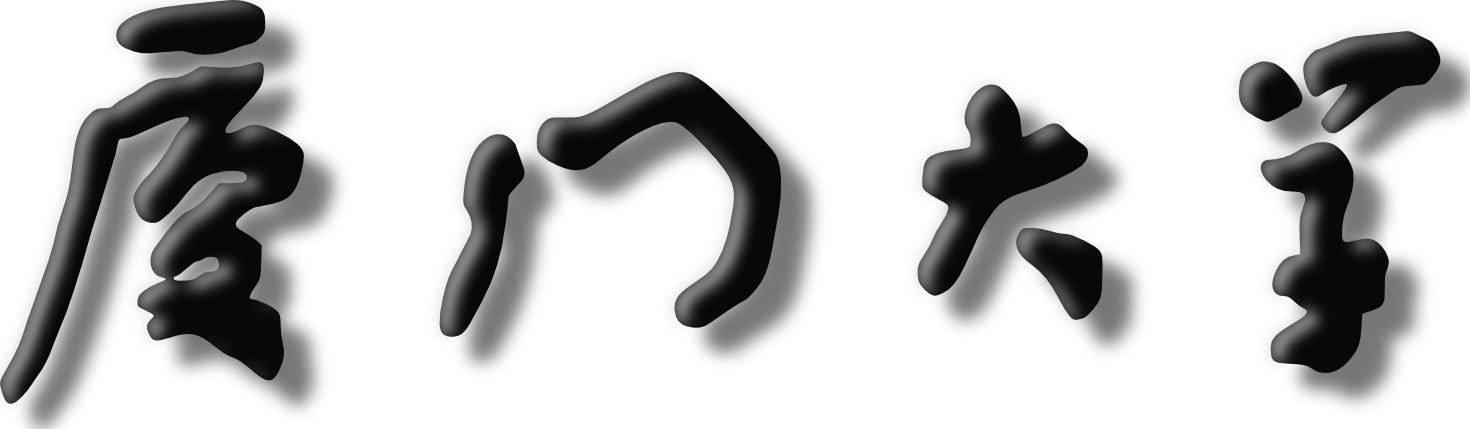
\includegraphics[width=5.8cm]{figures/xmu-zi-3d-600dpi}\\
      \vskip \stretch{2}
      {\rmfamily\bfseries\xiaoer
        \fillparbox{198pt}{\XMUT@value@degree%
        学位论文}\\
      }
      \vskip \stretch{2}
        {\sffamily\bfseries
          \erhao \XMUT@value@title
        }
      \vskip \stretch{1}
        {\rmfamily\bfseries
          \sanhao \XMUT@value@englishtitle
        }
      \vskip \stretch{2}
      \newlength{\XMUT@len@author}
      \settowidth{\XMUT@len@author}{\XMUT@value@author}
      \setlength{\XMUT@len@author}{\XMUT@len@author * \real{1.8}}
        {\ttfamily\mdseries\xiaoer
          \fillparbox{\XMUT@len@author}{\XMUT@value@author}
        }
      \vskip \stretch{1}
      %\def\tabcolsep{1pt}
      %\def\arraystretch{1.5}
      \newlength{\XMUT@len@advisor}
      \settowidth{\XMUT@len@advisor}{\XMUT@value@advisor\hspace*{1.5em}\XMUT@value@advisortitle}
      %% length for ~~
      %\addtolength{\XMUT@len@advisor}{30pt}
      \setlength{\XMUT@len@advisor}{\ifdim \XMUT@len@advisor > 84pt \XMUT@len@advisor
        \else 84pt
        \fi}

      {\ttfamily\mdseries\sihao
        \begin{tabular}{rl}
          \parbox[t]{6cm}{\hfill\fillparbox{84pt}{指导教师姓名}:}&%
            \parbox[t]{6cm}{~\fillparbox{\XMUT@len@advisor}{\XMUT@value@advisor~\XMUT@value@advisortitle}\hfill}\\
          \fillparbox{84pt}{专业名称}:&~\fillparbox{\XMUT@len@advisor}{\XMUT@value@major}\\
          \fillparbox{84pt}{论文提交日期}:&%
            ~\fillparbox{\XMUT@len@advisor}{\textrm{\XMUT@value@submitdate@year}~年%
              ~\textrm{\XMUT@value@submitdate@month}~月}\\
              %\makebox[3ex]{\textrm{\XMUT@value@submitdate@day}}日\\
          \fillparbox{84pt}{论文答辩时间}:&%
            ~\fillparbox{\XMUT@len@advisor}{\textrm{\XMUT@value@defenddate@year}~年%
              ~\textrm{\XMUT@value@defenddate@month}~月}\\
            %\makebox[3ex]{\textrm{\XMUT@value@defenddate@day}}日\\
          \fillparbox{84pt}{学位授予日期}:&%
            ~\fillparbox{\XMUT@len@advisor}{\textrm{\XMUT@value@grantdate@year}~年%
              ~\textrm{\XMUT@value@grantdate@month}~月}\\
              %\makebox[3ex]{\textrm{\XMUT@value@grantdate@day}}日
        \end{tabular}
      }
      \vskip \stretch{2}
      \rmfamily\mdseries\sihao
      \begin{tabular}{rl}
        \parbox[t]{7cm}{\hfill}&\parbox[t]{7cm}{
                \fillparbox{98pt}{答辩委员会主席}:~%
		\underlinewidth[75pt]{\texttt{\XMUT@value@chairman}}\hfill\\
                \fillparbox{42pt}{评阅人}:~\underlinewidth[131pt]{\texttt{\XMUT@value@appraiser}}\hfill
        }
      \end{tabular}
      \vskip \stretch{2.5}
        \XMUT@value@submitdate@year~~年%
          ~~\XMUT@value@submitdate@month~~月
          %\XMUT@value@submitdate@day 日
      \vskip \stretch{2}
    \end{center}
  \end{titlepage}
  %\cleardoublepage
  % 版权声明
  \chapter*{\centering{\sffamily\bfseries\xiaoer 厦门大学学位论文原创性声明}}
  \thispagestyle{empty}
  \begin{doublespace}
    \rmfamily\mdseries\sihao
    本人呈交的学位论文是本人在导师指导下,独立完成的研究成果。本人在论文写作
    中参考其他个人或集体已经发表的研究成果,均在文中以适当方式明确标明,并符
    合法律规范和《厦门大学研究生学术活动规范(试行)》。

    另外,该学位论文为(\@ifundefined{XMUT@value@team}%
    {\parbox[t]{200pt}{\quad}}{\XMUT@value@team})课题(组)的研究成果,获得
    (\@ifundefined{XMUT@value@fundteam}{\parbox[t]{120pt}{\quad}}%
    {\XMUT@value@fundteam})课题(组)经费或实验室的资助,
    在(\@ifundefined{XMUT@value@lab}{\parbox[t]{120pt}{\quad}}%
    {\XMUT@value@lab})实验室完成。(请在以上括号内填写课题或课题组负责人或
    实验室名称,未有此项声明内容的,可以不作特别声明。)

    \vspace{20pt}

    \hfill 声明人(签名):\hspace*{4cm}\\
    \vspace{-10pt}
    \hfill 年\hspace{26pt}月\hspace{26pt}日\hspace*{2cm}

  \end{doublespace}

  %\cleardoublepage
  \newcommand\XMUT@checkmark{\fillparbox{2em}{\centering\ensuremath{\checkmark}}}
  \chapter*{\centering{\sffamily\bfseries\xiaoer 厦门大学学位论文著作权使用声明}}
  \thispagestyle{empty}
  \begin{onehalfspace}
    \rmfamily\mdseries\sihao
        本人同意厦门大学根据《中华人民共和国学位条例暂行实施办法》等规定保留和使
    用此学位论文,并向主管部门或其指定机构送交学位论文(包括纸质版和电子版),
    允许学位论文进入厦门大学图书馆及其数据库被查阅、借阅。本人同意厦门大学将
    学位论文加入全国博士、硕士学位论文共建单位数据库进行检索,将学位论文的标
    题和摘要汇编出版,采用影印、缩印或者其它方式合理复制学位论文。

    本学位论文属于:

    (\ifthenelse{\boolean{XMUT@boolean@confidential}}{\XMUT@checkmark}{\hspace{2em}})
    \quad 1.\quad 经厦门大学保密委员会审查核定的保密学位论文,于%
    \@ifundefined{XMUT@value@confidentialdate@year}
    {\hspace{60pt}}
    {\XMUT@value@confidentialdate@year}年%
    \@ifundefined{XMUT@value@confidentialdate@month}
    {\hspace{28pt}}
    {\XMUT@value@confidentialdate@month}月%
    \@ifundefined{XMUT@value@confidentialdate@day}
    {\hspace{28pt}}
    {\XMUT@value@confidentialdate@day}日解密,解密后适用上述授权。


    (\ifthenelse{\boolean{XMUT@boolean@confidential}}{\hspace{2em}}{\XMUT@checkmark})
    \quad 2.\quad 不保密,适用上述授权。

        (请在以上相应括号内打“\ensuremath{\checkmark}或”填上相应内容。保密学位论文应是已经厦门大学
    保密委员会审定过的学位论文,未经厦门大学保密委员会审定的学位论文均为公开
    学位论文。此声明栏不填写的,默认为公开学位论文,均适用上述授权。)

    \vspace{20pt}

    \hfill 声明人(签名):\hspace*{4cm}\\
    \vspace{-10pt}
    \hfill 年\hspace{26pt}月\hspace{26pt}日\hspace*{2cm}

  \end{onehalfspace}
  %\clearpage
}
\makeatother

%---------------------------- 数学公式设置 ------------------------------%
%\setlength{\abovedisplayskip}{6pt plus1pt minus1pt}     %公式前的距离
%\setlength{\belowdisplayskip}{6pt plus1pt minus1pt}     %公式后面的距离
\setlength{\arraycolsep}{4pt}   %在一个array中列之间的空白长度, 因为原来的太宽了

% \eqnarray如果很长,影响分栏、换行和分页(整块挪动,造成页面空白),
% 可以设置成为自动调整模式
\allowdisplaybreaks[4]

%%%%%%%%%%%%%%%%%%%%%%%%%%%%%%%%%%%%%%%%%%%%%%%%%%%%%%%%%%%
%下面这组命令使浮动对象的缺省值稍微宽松一点,从而防止幅度
%对象占据过多的文本页面,也可以防止在很大空白的浮动页上放置
%很小的图形。
%%%%%%%%%%%%%%%%%%%%%%%%%%%%%%%%%%%%%%%%%%%%%%%%%%%%%%%%%%%
\renewcommand{\textfraction}{0.15}
\renewcommand{\topfraction}{0.85}
\renewcommand{\bottomfraction}{0.65}
\renewcommand{\floatpagefraction}{0.80}

\pagenumbering{roman}


\begin{document}
%% 确保zhspacing需要的符号定义没有被其他宏包改掉
\def\lq{`}\def\rq{'}
\zhspacing

%% 读入作者的信息
%% 中图分类号
\classification{T192}
%% 保密不?第一个参数是显示在封面上的,第二个参数是选择著作权使用声明中打哪个勾
\confidential{公开}{false}
%% 如果是保密论文,你可能想把保密日期一并填上
%\confidentialdate{2009}{9}{9}
\UDC{168}
\studentsn{20620061152XXX}
\degree{博士}
\author{练睿婷}
\school{厦门大学}
\title{Between Language and Logic: Comprehension, Generation and Reasoning Using Systems of Hypergraph Transformations Embedded in an Integrated Cognitive Architecture}
{Between Language and Logic: Comprehension, Generation and Reasoning Using Systems of Hypergraph Transformations Embedded in an Integrated Cognitive Architecture}
\advisor{江青茵}{教授}
\chairman{答辩主席}
\major{化学工程}
\submitdate{2009}{9}
\defenddate{2009}{9}
\grantdate{2009}{9}
\appraiser{老师一~~老师二}

%% 用在原创性声明中的
\team{化学化工学院~化工模拟优化及先进控制}
\fundteam{化学化工学院~化工模拟优化及先进控制}
%\lab{化学化工学院~过程控制实验室}


%% 加入pdf文件的关键字,\pdfkeywords必须在\maketitle之前才有效
\pdfkeywords{XeLaTeX;厦门大学硕博学位论文模板}

%% 生成a4封面、原创性声明、著作权使用声明
\maketitle

%% 正文默认使用小四,字号的定义在 config/headcommon.tex中
\xiaosi

%% 读入中英文摘要
\begin{abstract}

一个能理解、生成自然语言并能用自然语言流利交流的系统将会有广泛的用途,但目前的计算语言学软件几乎在所有关键领域的表现,都与人类的需求相差甚远。本文在自然语言理解、生成和对话系统方面展开了深入研究,旨在搭建一个以能实现智能对话为长远目标的自然语言处理工具集。

本文的工作主要在认知体系结构OpenCog上进行的,OpenCog是一个旨在实现通用人工智能(AGI)的集成软件平台,采用基于加权有向超图的知识表示体系Atomspace,不仅为自然语言过度到逻辑语义形式提供了平台,而且方便了常识推理和自适应学习机制等研究工作的开展。

在理论层面上,本文的核心研究问题是设计一个面向英语的智能会话系统,其中包含自然语言理解(将英语句子转换成逻辑表达形式)、自然语言生成(将逻辑表达式转换成英语句子)、面向超图的推理以及目标驱动的对话控制。本文对该设计的实现和相关的实验工作主要集中在自然语言理解和生成方面,使其成功地从设计阶段走向能实现很多实用功能的阶段。在推理和对话控制方面,我们也进行了相关实验,并搭建了一个能集成自然语言理解、生成、推理以及对话控制等模块的原型系统。

在技术层面上,本文的研究工作在以下四个假设中展开:1)借助一个超图转换系统,使用依存关系语法、传统逻辑与谓词逻辑的合理结合,将各式各样的自然语言表达转换成满足下列要求的逻辑表达方式,是可行的。2)借助由超图转换表示的推理规则和基于超图表示的知识库,使用简单的逻辑推理,在上述自然语言理解框架输出的逻辑表达式上实现基本的常识推理,是可行的。3)借助一个超图转换系统和一个超图匹配系统,在由自然语言理解系统自动生成的二元组(语言表达式,逻辑表达式)组成的知识库中根据逻辑表达式找到匹配的语言表达式并生成自然语言,是可行的。4)利用上述的语言理解、生成和逻辑推理系统,构建一个有用且灵活的智能会话系统,是可行的。

在自然语言理解方面,本文论证了一个可行的自然语言理解流水线,它集成了改进后的卡耐基-梅隆大学的链语法解析器、改进后的RelEx关系抽取系统以及一个全新的RelEx2Logic系统,能将RelEx的输出转换成OpenCog所使用的概率逻辑网络形式的逻辑表达式。在自然语言生成方面,本文在OpenCog系统内实现了一个全新的自然语言生成系统,通过微观规划和表层生成,能将一个给定的逻辑表达式转换成相应的英文句子。在基于语言的推理方面,借助于OpenCog中的概念逻辑网络(PLN)框架,以基于上述自然语言理解框架输出的逻辑表达式作为推理前提,本文实现了不同形式的逻辑推理实例。最后,本文论证了上述的集成系统框架能被应用在自然语言问题系统和智能会话系统中。

本文阐述的研究工作目前仍在继续,距离达到人类水平的智能会话系统的长远目标,还有很长的路要走。但是,本文的理论研究工作和相关的实用工具的开发,已经向着我们的长远目标迈出了一大步,无论是被应用在现实世界上的相关自然语言软件,还是在OpenCog的推理系统上实现的基于自然语言的常识推理,都在自然语言处理领域有着深远的意义。

\keywords{自然语言理解;自然语言生成;知识表示;对话系统}
\end{abstract}

\begin{englishabstract}
    A software program that could fluently understand, generate, and converse in natural language would have a huge variety of uses.   However, current  computational linguistics software falls far short of human performance in almost every key area required for achieving this functionality, e.g. language comprehension, generation and dialogue.   Our goal in undertaking the work reported in this thesis has been to build a conceptual and software toolset that will allow the construction of truly capable natural language processing software, with interactive dialogue as the main long-term application in mind.

We have carried out our work mainly within the OpenCog cognitive architecture, an integrated software platform designed with the goal of robust Artificial General Intelligence.   OpenCog's key feature is the representation of knowledge in a weighted, labeled hypergraph store called the Atomspace, which allows representation of knowledge in a language that is both rigorous in the sense of probabilistic logic, and relatively simple and commonsensical and amenable to automated learning mechanisms.   

On a theoretical level, the central problem we have confronted is the design of an English language dialogue system incorporating language comprehension (via mapping English sentences into logic expressions in the Atomspace format), language generation (via mapping Atomspace logic expressions into English sentences), logical reasoning on Atomspace logic expressions, and motivation-driven dialogue control.    Our practical implementation and experimentation work has focused mainly on the comprehension and generation portions of the design, which we have successfully brought from the design phase to the stage of adequate initial practical functionality.  We have also done some implementation and experimentation regarding the reasoning and dialogue control components, though our work there has been more at the research and early prototype level.

On a more technical level, regarding comprehension, generation and reasoning, we have aimed to explore the following hypotheses: 1) That it is viable to transform a wide variety of natural language expressions into logic expressions via a system of hypergraph transformations, using dependency grammar and an appropriate combination of term logic and predicate logic; 2) That it is viable to carry out a variety of simple logical inferences, using inference rules represented as hypergraph transformations and representing aspects of human commonsense reasoning, based on combining the logic expressions output by the above-described natural language comprehension framework; 3) That it is viable to transform a wide variety of logic expressions into natural language expressions, via a process comprising a system of hypergraph transformations and centered on matching against a knowledge base composed of (linguistic expression, logic expression) pairs formed via automated language comprehension; 4) That a framework incorporating items 1-3 can be utilized for natural language dialogue.

In the comprehension domain, we have demonstrated a natural language comprehension pipeline that chains together an improved version of the Carnegie-Mellon Link Parser, an improved version of the RelEx relation extractor system, and a wholly new system called RelEx2Logic that maps the output of RelEx into logic expressions in the Probabilistic Logic Networks utilized by OpenCog.    We have also demonstrated a novel natural language generation system, implemented inside the OpenCog system, which generates English sentences from a provided logic expression via a microplanning phase followed by a surface realization phase, where the surface realization process is based on matching fragment of the provided logic expression to fragments of logic expressions produced via comprehension using the above framework.   We have demonstrated the use of OpenCog's Probabilistic Logic Networks (PLN) framework used to carry out a variety of logical inference examples based on premises that are logic expressions obtained by interpreting English sentences according to the above comprehension framework.  Finally, we have shown that this integrated framework can be used for natural language question answering, a simple case of interactive dialogue.

The work reported in this thesis remains ongoing, and the long-term goal of a natural language dialogue system with full human-level functionality remains a significant way off.   However, the theoretical and practical tools created in the course of this thesis work constitute a significant step toward this long-term goal, and also possess significant value in themselves, both as tools for use in real-world software applications and as demonstrations of what kind of natural language processing it is possible to do using an OpenCog logic-based framework.

\englishkeywords{Natural Language Comprehension; Knowledge Representation; Dialogue System; Natural Language Generation}
\end{englishabstract}

%% 生成中英文目录
\tableofcontents

%% 以数字风格开始正文页码
\pagenumbering{arabic}

%words	formula
%a the	D+
%snake cat	D- & (O- or S+)
%chased	S- & O+
%% 读入各章节
\chapter{前言}{Preface}
\label{chap:intro}

目前,计算语言学软件几乎在每个关键领域都远远落后于人类的认知,如自然语言理解、生成和对话。计算语言学系统的功能在近几十年来得到稳步提高,在很大程度上是由于互联网的总体发展和相关的“大数据”现象所带来的语料库语言学的兴起。然而,在目前这么多研究方向中,哪一个最能带领该领域快速持续发展,还没有定论。

本文提出的结论,是遵循计算语言学功能发展的一个特定方向。本文工作是在一个旨在实现通用人工智能(AGI)的中集成认知体系中进行的,长远目标在于实现具有一定智能水平的自然语言理解、生成和对话系统。除此之外,本文也取得不依赖与该集成认知体系的具有价值的特定研究成果。

本文的研究在以下四个基本假设中展开。这些假设来源于,OpenCog通用智能系统 \cite{EGI1} \cite{EGI2}中的基于加权有向超图的知识表示以及基于超图转换的认知运算。这些假设可以简明地总结如下:

\begin{itemize}
\item {\bf 假设1——关于自然语言理解:}借助一个超图转换系统,使用依存关系语法、传统逻辑与谓词逻辑的合理结合,将各式各样的自然语言表达转换成满足下列要求的逻辑表达方式,是可行的。
    \begin{itemize}
    \item 包含自然语言表达式中的主要语义。
    \item 具体化自然语言表达式中存在的任何无法在语言到逻辑的转换消除的歧义,使得这些歧义能通过基于语境知识的逻辑推理后很直截了当地得到消除。
    \end{itemize}
\item {\bf 假设2——关于基于语言的推理:}借助由超图转换表示的推理规则和基于超图表示的知识库,使用简单的逻辑推理,在上述自然语言理解框架输出的逻辑表达式上实现基本的常识推理,是可行的。
\item {\bf 假设3——关于自然语言生成:} 借助一个超图转换系统和一个超图匹配系统,在由自然语言理解系统自动生成的二元组(语言表达式,逻辑表达式)组成的知识库中根据逻辑表达式找到匹配的语言表达式并生成自然语言,是可行的。
\item  {\bf 假设4——关于智能会话系统:} 利用上述的语言理解、生成和逻辑推理系统,构建一个有用且灵活的智能会话系统,是可行的。
\end{itemize}

本文提供了大量的证据支持前三个假设。完全吻合前三个假设,本文实现了能完成“英文—逻辑—英文”转换的软件系统。在这点上,我们还不能提供完整、全面覆盖英文中各种语言现象的系统。但目前没有一个计算语言学系统可以提供完整、全面覆盖任何一种自然语言。具体地可表现为:
\begin{itemize}
\item 对于假设1,本文论证了一个可行的自然语言理解流水线,它集成了卡耐基-梅隆大学的链语法解析器改进版本 \cite{Sleator1993}、RelEx关系抽取系统\cite{Goertzel2006}的改进版本 以及一个全新的RelEx2Logic系统——将RelEx的输出映射到OpenCog通用人工智能系统框架 \cite{EGI1}\cite{EGI2}所使用的概率逻辑网络(PLN)形式的逻辑表达式。文献\cite{Lian2012}中报道过这个框架的早期阶段;本文所述版本更为精准,功能更为强大。
\item 对于假设2,借助于概念逻辑网络(PLN)框架,以基于上述自然语言理解框架输出的逻辑表达式作为推理前提,本文实现了不同形式的逻辑推理实例。
 \cite{Goertzel2006}中已经尝试将PLN推理应用到自然语言理解的输出结果,但本文取得了比之前更专业更具体的实验结果。
\item 对于假设3,本文实现了一个全新的自然语言生成系统,该系统在OpenCog系统内实现,通过微观规划和表层生成,能将一个给定的逻辑表达式生成相应的英文句子,其中表层生成过程使用了逻辑表达式的匹配,这里的逻辑表达式正是上述自然语言理解系统中使用的语义表示方式。文献 \cite{Lian2010}阐述了该框架的早期阶段的实现原理和方法,本文所述版本对其做了大量的改进,框架更复杂,功能更为全面。

\end{itemize}
\noindent 对于假设4,本文展开了深入的理论研究和设计工作,并实现了一个相应的原型系统,会在第\ref{chap:dialogue}章中具体阐述。这也是我们目前和不久的将来的研究重点。


\section{基于规则的系统的优缺点}{Strengths and Weaknesses of Hand-Coded Rules}
在上述前三个假设前提下实现的软件系统主要是基于人工编写的语言规则(在理解方向上,生成过程依赖于隐式的理解规则,而不需要额外的规则)。然而,这不是本文所采用方法的全部。事实上,目前正在进行的无监督的语言学习,即希望能通过无监督的机器学习方法来从无标记的语料库获得的相关语法规则来替换人工编写的规则,这项工作将在第\ref{chap:unsupervised}章中论述。本文使用人工编写的规则库,不是把它作为智能英文处理系统的最终、全面的基础。我们认为,到最后,这也是一个不可行的方法,因为语言本身的复杂性,所需的规则数目将超越人工能操作的范围。相反,我们这里使用人工编写的规则库作为一个自然语言理解系统的“原型”,将架构问题从学习问题中分离出来,并提出一个语言理解和生成的通用且强大的架构。在这个架构内从学习更广泛的功能语言学内容到操作,作为一个独立的问题,将在第\ref{chap:unsupervised}章中进一步阐述。

在承认基于规则的方法的局限性的同时,值得肯定的是,该方法有着潜在的语用价值。从一个旨在开发一个能够在相对具体的语境中实现语言理解和/或生成的软件系统的程序开发者的角度来看,一个基于规则的自然语言处理系统可能是完全足够的,甚至在某些情况下有可能由于它的可预见性和简单性,成为最好的基于学习的系统。这里所描述的软件系统是以专业方式实现和架构的,并可以直接应用在现实世界中;事实上,该系统的好几个方面已经以这种方式被应用在一些商业软件中。\footnote{本文使用的关系抽取工具RelEx已经在一些由美国公司Novamente LLC和Linas AGI LLC签订的商业项目中被广泛应用,由于商业性质,我们无法在此提供相关参考文献。}

\section{OpenCog框架}{The OpenCog Framework}
如上所述,本文工作已在AGI软件框架OpenCog背景下实现。OpenCog在的自然语言处理和数据挖掘领域已被用于商业应用,如 \cite{Goertzel2006}。它也被用于虚拟世界中对虚拟智能体的控制\cite{Goertzel2008d}  \cite{Goertzel2011x},也被用于控制人形机器人\cite{Goertzel2010h}。

在文献\cite{GoertzelHP}中概述的“模式主义(patternist)”系统理论概念下,OpenCog以一种统一的体系结构融合了多种人工智能范式,比如不确定逻辑、计算语言学、进化编程学习和基于连接主义的注意力分配机制。这些范式都可以在一种通用的神经符号超图知识库上进行相互协作,这个超图知识库也就是所谓的原子空间Atomspace(”原子Atom“包括节点和链接,其中链接还包括超链接)。这些过程之间通过相互作用来激发Atomspace中高层网络结构的自发组织。后文将对OpenCog做更详细的讨论,读者也可参考 \cite{Goertzel2010h},或从 \url{http://opencog.org}获得更多相关内容。

从计算语言学的角度来看,OpenCog提供了以下主要模块:
\begin{itemize}
\item 高度灵活的知识表示框架(Atomspace以及其中包含的PLN原子类型),能直观的表达各种各样的句法和语义结构;
\item PLN逻辑推理引擎,可对自然语言理解框架的输出进行简单的推理;
\item 基于超图的模式匹配和以及在Atomspace上实现遍历工具,为Relex2Logic、微观规划以及表层生成等工具的开发,提供了便捷又实用的平台。
\end{itemize}

\section{存在的问题和未来的研究}{Omissions and Ongoing Development}
虽然上述工作已经取得了重要成果,但是从一个更广阔的视野来看,仍然还有很多未完成的工作,其中有许多也是我们目前正在研究和开发的课题。

首先必须强调的是,截止到我们目前所做工作为止,语言理解和生成的许多关键方面一直未被关注,甚至完全被忽略。如以下几个例子:
\begin{itemize}
\item 形态。链语法分析器,作为上述理解系统的初始阶段,最近已扩展到在语素及文字水平进行句法分析;但我们还没有将这项工作纳入到我们自己的工作中。
\item 语用。我们能够按照他们的实际能力对语句生成逻辑表达式进行分析,但是我们并未执行语用方面的分析。
\item 消歧。我们已在OpenCog框架中实现了一个简单词义消歧系统,但还没有集成到本文的工作中。
\item 名词的回指消解。在我们的理解系统内,人称代词的指代消解已通过各种启发式算法实现,但名词的回指却被忽略。
\end{itemize}

目前我们工作的一部分是指出整体框架中的这些缺陷。然而,我们相信即使给出这些疏漏,我们所做的工作也足够为以上三个假设提供合理的证据支持。展示处理上述现象能力必然有助于compelling system,但是对于验证本方法和三个假设的有效性并不必要。

本文工作的其中一个目标就是构建一个具有一定智力水平的智能会话系统。为了实现这样的智能会话系统,本文也开发了涉及自然语言理解、生成和推理等的相关模块。但本文的工作并不仅仅包括自然语言理解、生成和推理本身,例如还包括下面几个方面:
\begin{itemize}
\item 来自语言的逻辑表达和来自其他信息渠道的逻辑表达的有效整合,这些其他信息渠道可以是机器人或虚拟世界里的涉身知识,也可以是限定领域的标注语料库
\item “对话控制程序”的实现,该对话控制程序从一个动机驱动的系统中获取相关信号,然后结合系统当前的动机、最近的语言输入以及当前的系统知识等相关语境知识来选择相应的语言应答。
\item 额外的推理控制机制,使得智能体在被不相关或者不完全相关的信息来源打断后,仍能进行相对复杂的推理,从而给出相关的应答。
\end{itemize}

这些模块的当前现状将在第 \ref{chap:inference}和\ref{chap:dialogue} 章介绍。这些工作目前还无法在所有的语言现象中得到了验证,还有待进一步深入研究。然而, 在理解、生成和推理等方面,明确的研究方向和相关工具的实现,无疑为以后的研究奠定了结实的基础和提供了一个便捷的研究平台。我们提出三个核心假设的主要原因,是因为它们提供了一种有效的方法,能够借助自然语言理解、生成和语义推理等子系统,来搭建一个大型的智能对话体系结构。

%%\chapter{自然语言处理的研究现状}{The State of the Art in Natural Language Processing}
\label{chap:review}

     近年来,自然语言处理(NLP)逐渐成为人们越来越关注的领域。它融合了计算机科学、语言学,以及其它学科。本文涉及了NLP领域中各个不同的研究方向,因此无法在短篇幅内给出每个方向的所有相关文献综述。Jurafsky的书 \cite{Jurafsky2009}已对这一领域进行了概述。在这一章中,我们将对众多NLP相关领域的研究现状进行大致的回顾,同时对NLP中的几个与我们的工作密切相关,或者具有可比性的研究方向和理论进行比较深入的探讨。在简要的研究历史回顾后,我们会总结自然语言理解、自然语言生成、对话系统、以及语义上的知识表示方面的未来发展趋势以及主要存在的问题。

\section{关于有效的可计算的语言处理的探索}{The Quest for Effective Computational Language Processing}

      从人工智能发展的早期开始,人们已认识到NLP在机器智能领域的关键性作用。在1950年,Alan Turing发表了他的那篇经典文章“计算机与智能化(Computing  Machinery and Intelligence)”。在文章中,他提出了一个理论,现在我们称其“作为智能标准的图灵测试”。他并没有称之为“自然语言处理”,但对于任何系统来说,要通过图灵测试,NLP显然是至关重要的。

人工智能方面的先驱在早期过于乐观,在自然语言处理方面也是如此。1954年,乔治城大学(Georgetown University)进行了一项试验,他们利用机器翻译将60多个俄语句子翻译成英文。这个试验的发起人声称:在3年或5年内,机器翻译将不成问题。然而,到1966年,一份报告显示:持续10年的研究都没有取得多少进展,而用于机器翻译的研究资金也大幅减少。事实上,在之后的15-20年里,机器翻译一直停滞不前,直到人们发现了完全不同的“统计语料库”分析法。
通过基于规则的对话系统,人们取得了初步进展。例如聊天机器人心理医生ELIZA\cite{Weizenbaum1966}和用于受限“积木世界(blocks worlds)” 的自然语言系统SHRDLU\cite{Winograd1972}。图 \ref{fig:eliza}中是ELIZA的对话例句。

\begin{figure}[htb]
\centering
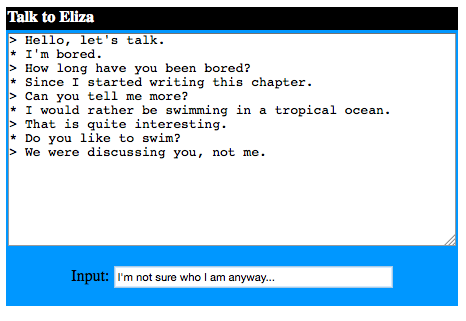
\includegraphics[width=14cm]{figures/eliza.png}
\caption{ 对话例句。这是与知名的聊天机器人心理医生ELIZA对话的现代版本。请注意:当“她”不知道该怎样回答的时候,“她”是如何转移话题的。 }
\label{fig:eliza}
\end{figure}

尽管这些系统看起来很聪明,甚至有些像人类的思维,但它们显然缺乏对它们所使用的语言的深度理解,而且至今,类似的对话系统也没有比这些早期的原型系统懂的更多。

在20世纪70年代,为了克服早期这些基于规则的聊天机器人的缺陷,许多程序员开始编写“概念本体知识库”,这些知识库将真实世界的信息转换为计算机可以理解的数据,以便聊天机器人获得更多的知识 \cite{McCorduck2004}。相对来说,在20世纪70年代早期,基于知识本体的“问答”(QA)系统在限定的领域内是成功的,例如LUNAR系统。它能够回答那些对阿波罗登月任务 \cite{Woods1973} 中带回的岩石进行地质分析的问题。(例如:高碱性岩石中铝元素的平均浓度是多少?)。 1971年的月球科学会议展示了LUNAR系统。当时,对于没有经过该领域训练的人提出的相关问题,LUNAR能够答出90\%。在之后的几年间,更多基于限定领域的问答系统相继出现。这些系统的共同特点是:都有核心数据库,或由相关领域的专家人工编写的知识系统。LUNAR和当时其它一些系统的语言能力只能与ELIZA的语言能力相提并论。

经过20世纪70年代和80年代的发展,NLP系统已能够融入了更先进的语言学理论,例如20世纪80年代末期,由加州伯克利大学Robert Wilensky 教授开发的Unix Consultant (UC)\cite{Wilensky88theberkeley}。UC以大量人工书写的知识库为基础,可以回答与Unix操作系统有关的问题。它会根据它对不同对话人所提出的问题的理解,组合出不同的答案。这种系统正是目前受限领域的自然语言问答系统(例如用于健康和生命科学的EAGLi \cite{eagli})的前身。

在这一时期,理论语言学和实用计算NLP之间的关系是错综复杂的,甚至有些麻烦。主流的理论语言学主要是基于Noam Chomsky的理论,这个理论的中心是:假定句子的“表层结构”能微妙地转换成“深层句法结构”。尽管人们进行了大量尝试,但发现这些理论并不适合计算机应用\cite{McCorduck2004}。

在NLP的发展历程中,最具革命性的事件是大型文本和语音语料库的出现,以及统计分析方法的发展。基于统计的NLP的目标是通过识别和判定这些语料库中的各种模式,来实现语言处理功能。这些方法的流行主要是由于计算机和通讯技术的进步,以及人们越来越多地使用光盘,紧接着互联网,而并不是因为NLP本身的发展。由于人们对作为训练语料库的平行文本语料库的使用,并在训练语料库上使用相对简单的统计学习算法,例如基于隐马尔科夫模型 (HMMs)\cite{Hutchins2005},机器翻译出现了重大进展。由Chomsky的早期导师Zellig Harris \cite{Harris1957}引领的标注语料库创建工作在众多实践中脱颖而出,同时一个有助于“有监督学习”任务的大规模分支领域出现了。例如:利用统计工具从标注语料库中学习语法,语料库中的每个句子都有人工标注的句法结构;或者使用人工标注的词性标注语料库,利用统计工具对新的文本进行自动词性标注。

“从大规模语料库中进行无监督学习”也是自然语言处理的研究重点(例如\cite{Spitkovsky2013}),但事实证明这更加困难。而“半监督式学习”则是相对成功的。它融合了标注语料库和网络中大量非标记文本的使用\cite{Abney2007} \cite{Guo2014}。


\section{自然语言理解}{Comprehension}

自然语言理解是NLP的分支领域,它是通过使用软件来理解自然语言的意义(语音,或者本文更关注的“文本”)。自然语言理解主要是将自然语言转换成抽象的语义形式,以获取语言的含义;或者是转换为某种响应(例如对某个问题的回答),以说明其理解了语言的含义。

\subsection{句法分析}{Syntactic Parsing}

通常自然语言理解是通过对句子的某些,或全部句法法进行分析来完成的。大量的形式化体系和算法通过它们自己的独特方式对句子的句法结构进行解析。大体来说,这些可以归类为“依存语法(DG)”对“短语结构语法(PSG)”。PSG首先对句子进行短语分析,然后指出单词和短语之间的关系,以及短语之间的关系;另一方面,DG仅仅在句子中的单词之间标注(有标记的)连接关系。后者(DG)是我们要在本文中探讨的语法类型。


这里的“依存”是指语言单位(如单词)由有向链接相互联系在一起。一般来说,在DG中,(限定)动词被视为句子或子句结构的中心,其它所有句法单位(单词)是直接或间接地与动词通过有向链接相连。这种有向链接被称为“依存”。句子结构是由一个词(中心词)与它的依存词之间的关系而决定的。


“依存”关系是一对一的对应关系:对于句子中的每个元素(例如:单词或语素)来说,实际上句子中都有一个与其相对应的节点。这种一对一的对应关系决定了“依存语法”就是单词(或语素)的语法。所有的句子都有元素和将元素组成结构的依存关系,这种情况应该与短语结构语法的“成分关系”进行比较,“成分关系”是一对一,或一对多的对应关系,也就是说,对于句子中的每个元素来说,有一个或多个与其对应的节点。这种不同带来的结果是:相比短语结构,依存结构非常紧凑,因为它往往包含很多小的节点。从计算机处理的角度来说,这种简洁的结构是有益的。


\subsection{关系抽取}{Relationship Extraction}
自然语言理解中的一个重要方向是{\bf 关系抽取}。在NLP领域中,关系抽取已成为一个重要的研究方向,一方面是因为它的实际应用价值,另一方面因为它被看做是语义分析的一部分,而且是目前的技术相对容易实现的那部分。到目前为止,吸引最多注意力的关系抽取是命名实体之间的关系识别,例如:“个人从属关系”和“组织地址关系”。

一般来说,关系可以由一个元组的形式来定义的,$t = (e_1, e_2, ...,e_n)$。在这里,$e_i$ 是文本中预定义关系$r$ 的实体。大多数关系抽取系统主要关注二元关系的抽取。例如 :

\begin{verbatim}
位于(厦门,中国)
father-of(Richard Li, Li Ka-Shing)
\end{verbatim}

抽取“高阶关系”也非常有意义。例如这个句子:``At codons 12, the occurence of point mutations from G to T were observed'' (“在密码子12,观察到从G到T的点突变”)。句子中出现了一个4进制生物医学关系,可以描述为:

\begin{verbatim}
point mutation(codon, 12, G, T)
\end{verbatim}

目前人们普遍视“关系抽取”为一个有监督分类问题,它从一个语料库开始(语料库中包含由人类标记的相关语义关系),然后利用统计方法来对标记的关系建模,并学习出适合应用于其它文本的统计模型。

目前,关系抽取系统的主要限制在句子层面上运用。事实上,关系可能跨越句子,甚至贯穿不同的文件。然而,解决这一问题需要一定的常识和非常灵活的知识表示。本文的研究也无法直接解决这一问题,但我们相信:通过将句子意义映射为通用的知识表示,我们已经奠定了解决问题的基础。在这种知识表示中,跨句或跨文本的通用联系和推理是可以被实现的。

\subsection{流结构语法}{Fluid Construction Grammar}

将流结构语法(FCG)与本文使用的语言形式化体系进行比较分析是很有意义的。在FCG中,一句话语的信息是以语义和句法结构组织在一起的。语义结构是对“话语意思”的分解,它含有特定语言的语义分类,例如:“put”事项被归类为“起因-移动-位置”类事项,包括一个施事者(agent)、一个受事者(patient)和一个位置(location)。句法结构是将话语形式分解为成分和词素,还包含附加的句法分类,比如:句法特征(例如:数量和性别)、词序限制等。


从理论上来说,FCG是基于一种程序性语义的方法,在这个意义上,话语的意思是听话人假定要执行的程序,因此,概念化便是一个规划过程(规划该程序),而解析便是对该程序的执行过程。
FCG中,有关配对句法和语义结构的例子(短语“the ball”),请见图 \ref{fig:fcg1} and \ref{fig:fcg2}。

\begin{figure}[htb]
\centering
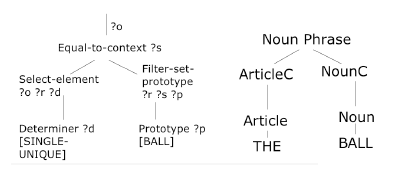
\includegraphics[width=12cm]{figures/fcg1.png}
\caption{ FCG syntactic and semantic structure for "the ball" }
\label{fig:fcg1}
\end{figure}

\begin{figure}[htb]
\centering
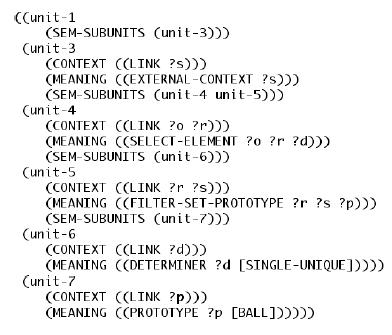
\includegraphics[width=12cm]{figures/fcg2.png}
\caption{ FCG semantic structure for "the ball" in  list format}
\label{fig:fcg2}
\end{figure}


所有的FCG规则都是双向的。通常在产生过程中,所要表达的语义内容是与语义结构相统一的,有可能产生一组绑定。如果成功了,绑定会与语义结构相融合。这种融合可以理解为“部分统一”,但它利用结构中那些遗漏部分扩展了结构。在句法分析过程中,被分析的句子与句法结构是统一的,同时,结果中的某些部分被添加到语义结构中。


这篇论文所提出的形式化体系在概念上有些类似FCG。 此外,我们有配对句法和语义结构,而且还进行双向处理。在第\ref{chap:comprehension}章中,我们将论述链语法,它将句子转换成句法结构,以及RelEx和RelEx2Logic模块,它们将句法结构转换成语义结构。在第 \ref{chap:generation}章中,我们将论述Microplanner 和SuReal模块,从另一个方向,将语义结构转换成句法结构,再生成句子。OpenCog中的模式匹配器(Pattern Matcher)使用我们的句法和语义结构时,也将这些结构视为有效的程序,同样实现了“程序性语义”。

我们的形式化体系与FCG的着重点不同。FCG主要是用作探索问题的理论工具,而我们所做的OpenCog系统则是用于真实世界的实际应用。

\section{知识表示}{Knowledge Representation}

对于任何以实现复杂功能(如对话系统或复杂的问答系统)为目标的NLP系统来说,该系统如何表达内部知识是非常关键的。先进的NLP功能一般要求从多个句子中获得互相关的信息,这通常需要持续存储那些从多个句子中抽取的信息。这种存储机制必须能够支持相当灵活的语义知识操作。上节我们看到的例子是FCG使用的基于逻辑的语义表达形式。在本文的研究中,我们将使用一种不同的逻辑表达形式,即OpenCog中概率逻辑网PLN(Probaabilistic Logic Networks)的形式体系。

\subsection{逻辑知识表示的优缺点}{Strengths and Weaknesses of Logical Knowledge Representation}

根据Pei Wang \cite{Wang2006}的理论,总体来说,逻辑推理系统通常包括以下组成部分:

\begin{itemize}
\item 一种形式化语言, 能用于知识表示,以及系统与其环境之间的沟通。
\item 一个语义系统,用于决定词的意义和句子真值。
\item 一套推理规则,匹配问题和知识,能从前提推出结论等。
\item 一个存储器,可以储存问题和知识,并提供推理的工作空间。
\item 一个控制机制,负责选择前提和每一步推理中需要的推理法则。
\end{itemize}

\noindent 前3个通常被认为是逻辑,或推理系统中的逻辑部分,最后的2个则被认为是推理系统中的控制部分。

使用逻辑来表达自然语言的语义,这涉及精确度和灵活度之间的平衡。逻辑是精确的,它的标志是“确定”。它带来一种用作定理证明的思考方式。它的优势在于稳定和系统的方式对表达式赋值并保持表达式的真值。在几乎没有歧义的技术领域,精确度是非常重要的,而逻辑显然是一个极好的架构。但是,当逻辑在意思和真值都比较模糊和模棱两可的领域中应用时,其适用性就不那么明显了,而且在人工智能和NLP领域中,逻辑的应用也常常引起争议。

进一步来说,逻辑领域中最长和最丰富的传统是以演绎推理为中心的。演绎推理是有限的推理形式,而且人们很少做关于自然语言的常识性推理,但仍然有大量的“归纳逻辑”\cite{Muggleton1994} \cite{Holland1989}工作(包括最近人们重视的“概率归纳逻辑编程” \cite{Riguzzi2014}和溯因推理\cite{Queiroz2005} \cite{Menzies1996})。这些推理方法也大量存在于我们所用的PLN系统中。


\subsection{谓语逻辑 VS 传统逻辑}{Predicate Logic vs. Term Logic}

在数学和NLP环境下,最普遍的逻辑形式是“谓语逻辑”。它的独特之处是对变量的使用,这些变量可以被量化。两个常见的限量词是存在量词$\exists$(“存在”)和普遍量词$\forall$(“所有”)。在谓语逻辑公式中,变量可能是人们谈及的宇宙元素,也许是超越宇宙的关系或函数。举例来说:在标准的谓语逻辑中,一个句子,例如“Ravens are black” (乌鸦是黑的),它呈现的是个“一般命题”,如:

$$
(\forall x)(乌鸦(x) \rightarrow 黑色(x)).
$$

谓语逻辑通常与语义学的“理论模型”法一同出现,它视“逻辑公式”为特定领域的模型\cite{Muller2009}。


另一个方法是“传统逻辑”推理法,这个概念实际上可以追溯到亚里士多德。在这里,“基本假设”是:命题由两个词语构成,推理过程反过来根据命题来构建。详解如下:

\begin{itemize}
\item 一个“词语”是言语表达的一部分,但就其本身而言,并没有对或错,例如“男人”或“凡人”。
\item 一个“命题”包含两个词语,其中一个(“谓语”)是对其它词(“主语”)的“证实”或“否认”。它能够反应“真”或“假”。
\item “三段论”是一种推理法,其中的一个命题(“结论”)必须遵循另外两个(“前提”)。
\end{itemize}

在“传统逻辑”推理法中,我们可以这样推理:

\begin{eqnarray*}
raven \rightarrow black(乌鸦 \rightarrow 黑色)
\end{eqnarray*}

无需引入量词。

以下是一个标准的“三段论”逻辑推理示例:

\begin{eqnarray*}
A \rightarrow B \\
B \rightarrow C \\
所以\\
A \rightarrow C
\end{eqnarray*}


这也是演绎推理的简单形式。
在人工智能领域,Pei Wang的NARS引擎运用了传统逻辑推理法\cite{Wang2006},并引入了独特的数学运算,用于管理与“传统逻辑关系”有关的不确定性。NARS是建构在经验的基础上,而不是模型论语义学。

在许多方面,我们所使用的PLN逻辑形式化体系与NARS有类似的地方,但也存在巨大差异。PLN在一个独特的数学框架下,同时利用传统逻辑和谓语逻辑。此外,PLN还使用概率数学,以推导不确定真值的公式。反之,NARS是基于原始的、非概率的、不确定的管理体系。PLN也是以经验语义为基础,但形式与NARS不同。


图\ref{fig:nars}展示了基本演绎推理、归纳推理和外展推理公式。这些公式是PLN和NARS共有的。在每个关系式右边的$<s,c>$表示“每个关系的优势和信心”。PLN和NARS使用不同的公式,从那些前提中推导(优势、信息)结论的真值。

\begin{figure}[htb]
\centering
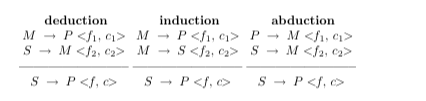
\includegraphics[width=12cm]{figures/nars.png}
\caption{ NARS/PLN term logic deduction, induction and abduction inference forms }
\label{fig:nars}
\end{figure}

\subsection{Cyc系统}{Cyc}

在NLP系统中,也许开发最彻底的“谓语逻辑”是由Cycorp公司开发的商用系统Cyc\cite{Lenat1990}。Cyc系统拥有一个非常丰富的人工编码知识库,它的终极目标是:以谓语逻辑的形式,将所有人类常识进行编码。虽然它的知识库中已存有数百万的谓语逻辑公式,但到目前为止,似乎只对一小部分人类常识进行了编码。 不过,作为智能应用系统,Cyc已经相当成功了。

我们之所以在这里讨论Cyc“知识表示”的基础,是为了与我们的系统进行比较。在Cyc系统中,概念名称被称作“常量”。在书写时,它们以"\#\$"开始。以下是几种常量:

\begin{itemize}
\item 单个词汇被称为“个体词”,例如:\#\$BillClinton (比尔·克林顿 或 \#\$France(法国)。
\item 集合词,例如\#\$Tree(树)-ThePlant(植物) (包括所有的树) 或 \#\$EquivalenceRelation (等价关系)(包括所有的等价关系)。
\item 真值函数,可以运用到一个或多个概念中,并反馈“真”或“假”。例如:\#\$siblings is the sibling relationship,如果两个参数是siblings,那就是真的。按照惯例,真值函数以小写字母开头。真值函数可能会被分拆为逻辑连接词(如:\#\$and, \#\$or, \#\$not, \#\$implies)和量词(如:\#\$forAll, \#\$thereExists等)。
\item “函数”能够从给定的词中生成新词汇,例如:
\#\$FruitFn,当提供了一个描述某种植物类型(或集合)的参数,它会给出这类植物的一组水果。按照惯例,“函数常量”以“大写字母”开始,以字符“Fn”结束。
\end{itemize}

“常量”之间由谓语联系在一起。最重要的谓语是: \#\$isa 和 \#\$genls。第一个(\#\$isa)描述的是:某个个体是某个集合中的一个例子(如:specialization);第二个(\#\$genls)描述的是:一个集合是另一个集合的子集合(例如:generalization)。
利用特定的CycL句子,我们可以得出概念事实。谓语是写在它的参数之前的,在圆括号内。例如:

 {\tt\begin{small}\begin{lstlisting}
    (\#\$isa \#\$BillClinton \#\$UnitedStatesPresident) \;
    \end{lstlisting}\end{small}}

\noindent 意思是 "Bill Clinton belongs to the collection of U.S. presidents" ;

 {\tt\begin{small}\begin{lstlisting}
    (\#\$genls \#\$Tree-ThePlant \#\$Plant) \;
    \end{lstlisting}\end{small}}
    
\noindent 意思是 "All trees are plants"; and 

 {\tt\begin{small}\begin{lstlisting}
    (\#\$capitalCity \#\$France \#\$Paris) \;
    \end{lstlisting}\end{small}}
    
\noindent 意思是 "Paris is the capital of France."


下面是比较封复杂的例子,它表示了一组或一类词的规则,而不是任意特定的个别词:

 {\tt\begin{small}\begin{lstlisting}
 (\#\$relationAllExists \#\$biologicalMother 
 \#\$ChordataPhylum \#\$FemaleAnimal)
    \end{lstlisting}\end{small}}
    

Cyc知识库被分为多个“微理论”库,它们是概念和事实的集合,每个“微理论”库都与一个特定领域相关联。每个“微理论”库都不能有相互矛盾的信息,而且可以通过Bayesian网络提供概率真值。

Cyc配备了一个复杂的、基于短语结构语法的NLP系统,这个系统将自然语言句子映射为Cyc逻辑形式。由于这个系统本身的特性,我们尚不清楚它到底具有什么样的优点和缺点。


\subsubsection{ConceptNet}{ConceptNet}

知识表示的另一个模式是由ConceptNet提供的\cite{Liu2004}。它从Cyc系统和形式逻辑中借鉴了一些理念,但没有考虑复杂的位元,如量词,并且比较接近自然语言层面。ConceptNet 是个大规模的语义网络,它表达概念(由单词或短语表述)之间的关系。图\ref{fig:concept}是关于子网络的例子。

\begin{figure}[htb]
\centering
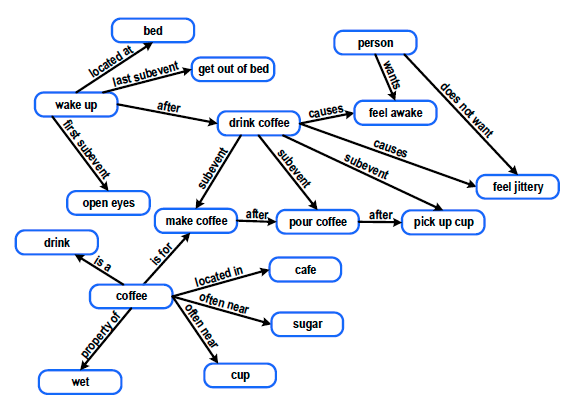
\includegraphics[width=12cm]{figures/conceptnet.png}
\caption{ An illustrative fragment of ConceptNet }
\label{fig:concept}
\end{figure}

ConceptNet系统的节点是自然语言碎片,这些碎片按照某个句法模式的本体进行了半结构化。它们适合一阶概念(作为名词短语,如potato chips)和二阶概念(作为动词短语,如:buy potato chips)。

节点可以由19个语义关系相连接:
\begin{itemize}

\item 事物 
\begin{itemize}
\item IsA ?(corresponds loosely to hypernym in WordNet)
\item PropertyOf ?(e.g. (PropertyOf ``apple'' ``healthy''))
\item PartOf ?(corresponds loosely to holonym in WordNet)
\item MadeOf ?(e.g. (MadeOf ``bottle'' ``plastic''))
\end{itemize}

\item 事件 
\begin{itemize}
\item FirstSubeventOf, LastSubeventOf ?(e.g. (FirstSubeventOf ``act in play'' ``learn script''))
\item EventForGoalEvent ?(e.g. (EventForGoalEvent ``drive to grocery store'' ``buy food''))
\item EventForGoalState ?(e.g. (EventForGoalState ``meditate'' ``enlightenment''))
\item EventRequiresObject ?(e.g. (EventRequiresObject ``apply for job'' ``resume''))
\end{itemize}

\item 动作 
\begin{itemize}
\item EffectOf ?(e.g. (EffectOf ``commit perjury'' ``go to jail''))
\item EffectOfIsState ?(e.g. (EffectOfIsState ``commit perjury'' ``criminal prosecution''))
\item CapableOf ?(e.g. (CapableOf ``police officer'' ``make arrest''))
\end{itemize}

\item 空间 
\begin{itemize}
\item OftenNear ?(e.g. (OftenNear ``sailboat'' ``marina''))
\item LocationOf ?(e.g. (LocationOf ``money'' ``in bank account''))
\end{itemize}

\item 目标 
\begin{itemize}
\item DesiresEvent, DesiresNotEvent ?(e.g. (DesiresEvent ``child'' ``be loved''))
\end{itemize}

\item 功能
\begin{itemize} 
\item UsedFor ?(e.g. (UsedFor ``whistle'' ``attract attention''))
\end{itemize}

\item 通用 
\begin{itemize}
\item CanDo ?(e.g. (CanDo ``ball'' ``bounce''))
\item ConceptuallyRelatedTo ?(e.g. (ConceptuallyRelatedTo ``wedding'' ``bride'' ``groom'' )
\end{itemize}
\end{itemize}


OpenCog的Atomspace是本文的研究重点,它与ConceptNet有些共同之处。我们视Atomspace为“加权标记超级图”,但ConceptNet只是一个“加权标记图”。此外,在可以直接表示的关系复杂性方面,Atomspace与ConceptNet有所不同。Atomspace包含与ConceptNet相似的简单节点和链接,但还有更加复杂的,且能够表示量词关系,还含有可执行程序等。它的设计原则是:先利用简单的、ConceptNet类的方法,尽可能地表示,但之后在必要的情况下使用更复杂的表示工具。大多数“表示工具”都来自传统逻辑,而不是谓语逻辑,但必要时也使用与“明确量词关系”相对应的节点和链接。


\section{语言生成}{Generation}

自然语言生成(NLG)是NL的反向过程。NLG是从信息的计算表示中自动生成人类(自然的)语言。大体上,NLG系统与以下问题有关:

\begin{itemize}
\item What should I say?(我应该说什么?)
\item How should I say it?(我应该怎么说?)
\end{itemize}

这涉及许多相互关联的计划过程,如:
\begin{itemize}
\item 决定要说的信息
\item 构建语篇计划
\item 将信息块转换为语篇单位
\item 选择适当的短语和单词
\item 输出正确的语法
\end{itemize}

将这个流程分解为阶段的方法如下:
\begin{enumerate}
\item 宏观计划
\item 微观计划
\item 表层实现
\end{enumerate}

宏观计划涉及选择和组织内容。它输入的是一个或多个沟通目标:解释、描述,或提问;引起听众的某种行动或思考等。宏观计划输出的是一种知识架构,这个架构不一定是语言的属性,而是体现智能体所要沟通的信息。除了一般性内容,这种知识架构可能包含一些与沟通过程有关的信息,例如:不同的知识块应该以什么样的顺序来传达。

有些宏观计划法涉及语篇结构的特定理论,例如:修辞结构理论\cite{Mann1987}。在本文所介绍的研究中,我们采用了宏观计划,利用名为“OpenPsi”的“动机认知模型”(这个模型的构建密切遵循人类心理学)。

微观计划则运用知识架构,并将它们分为句块。微观计划必须处理多种语言问题,例如:

\begin{itemize}
\item 句子范围:是否可以将两片叶子接在一起,怎样接在一起。(“我今天饿了。我去了 Burger King。” VS “我今天饿了,所以我去了Burger King。”)
\item 代词化
\item 聚合:删除重复内容。(“抽烟对你不好。抽烟会缩短你的寿命。抽烟让你口气不佳” VS “抽烟对你不好、缩短你的寿命,而且让你口气不佳”)
\item 主题化
\item 主题排序
\end{itemize}

到目前为止,我们的大多数微观计划都是为特定的应用而专门制定的。有一个名为SPUD\cite{Stone 1997}的多用途微观计划框架,它利用的是一个基于逻辑的计划流程形式。尽管在细节上有所不同(原来的SPUD是基于树-邻近语法),但我们所描述的微观计划在概念上受到了SPUD的很大影响。

最后,“表面实现”涉及的是文本表层的生成,例如:把知识结构转换为句子。经典的表层生成器,例如FUF/SURGE\cite{Elhadad1992}和 Penman/KPML\cite{Matthiessen1991},都是以深层语言学理论为基础的。其他知名的系统,例如Nitrogen\cite{Langkilde1998}则采用的是统计法。所有基于规则的方法和统计法现在仍然流行。

一般来说,与NL理解相比,NL生成技术要落后得多。目前的实用系统往往比较专业化,而且很粗糙。概念比较先进的系统,如FCG,尚未经过广泛地实践测试。正如第\ref{chap:generation}章中所介绍的,我们在这一领域的研究代表了“基于规则的方法”和“统计法”的融合。我们认为这种融合非常有前景,但还没有精细化,也没有经过系统性评估。

\section{问题回答}{Question Answering}

就连接NL理解、生成和知识表示而言,也许最简单、最有意义的模式就是“问题回答”。问答(QA)系统让使用者以自然语言提问,然后以自然语言响应。


许多现代QA系统基本上都是以文档为驱动的信息检索系统,请见图\ref{fig:qa}中的示例\cite{Hirschman2001}。这种系统(其中的问题被直接提交至一个大规模文本语料库)的表现通常优于20世纪70年代的早期QA系统(依赖人工编码的知识库)。

\begin{figure}[htb]
\centering
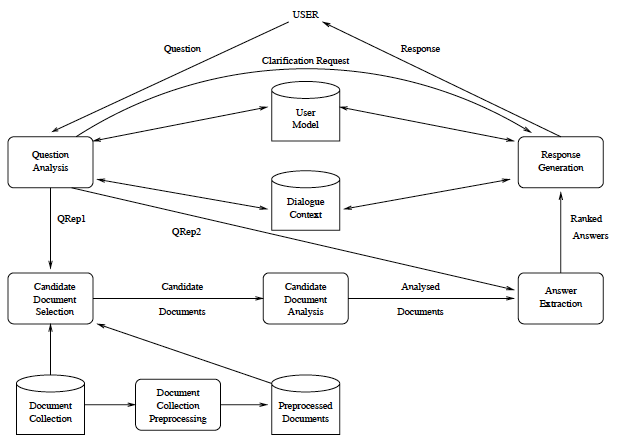
\includegraphics[width=12cm]{figures/qa.png}
\caption{典型的文件驱动问答系统的架构}
\label{fig:qa}
\end{figure}

这种以文件为驱动的QA系统通常包括一个问题分类模块。这个模块确定问题和回答的类型。分析问题之后,系统一般会运用几个模块。文本的数量逐步减少,这些模块则越来越多地应用于复杂的NLP技术。因此,文件检索模块可以使用搜索引擎来识别那些可能含有“答案”的文件,或文档中的段落。随后,一个过滤器预先挑选出包含同类字符的小文本碎片,用作预期回答。例如:如果问题是“谁发明了青霉素?”,过滤器会反馈包含人名的文本。最后,一个“回答抽取模块”会在文本中进一步寻找线索,以确定候选的答案是否能正确地回答这个问题。

另一方面,如果问答系统会根据对文本知识的深层理解来做出响应,那么“快速处理文本来响应问题”就不是一个非常可行的策略。更准确地说,用于为QA系统提供知识的文件必须预先由一个NL理解系统彻底地“读”和理解。后面的那个方法是我们要在本文的第\ref{chap:dialogue}章中探讨的。我们开发了一个简单的QA系统,它是一个整体互动对话体系的一部分。

在2010年,IBM的问答系统Watson以极大的优势击败了另两个Jeopardy冠军奖的获得者:Brad Rutter 和 Ken Jennings。Watson综合利用了信息检索法和基于推理的先进方法\cite{Ferrucci2011},可以说是迄今为止最先进的问答系统。

\subsubsection{问答系统的关键问题}{Key Issues Regarding Question Answering}

问答系统是一个复杂的探索课题,它涉及众多问题。举例来说,有证据表明:某种问题要难于其它问题。询问“为什么”和“怎样”的问题往往比询问“是什么”和“在哪里”的问题更难回答,这是因为它们要求对因果关系,或instrumental关系的理解。这些关系通常由分句或独立的句子来表达\cite{Hirschman1999}。

在2002年,一组研究人员绘制了一幅关于问答系统的研究路线图\cite{Burger2002}。他们当时提出的问题在今天仍然与我们息息相关。以下是他们发现的问题:

\begin{itemize}
\item 问题类别:不同类型的问题(例如“列支敦士登的首都是哪里?” VS“为什么会形成彩虹?”VS“玛丽莲·梦露和加里·格兰特出演过同一部电影吗?”)要求使用不同的策略来发现答案。
\item 问题处理:相同的信息可能是用不同的方式 来表达的,有些是疑问句(“莱索托国的国王是谁?”),有些是祈使句(“告诉我莱索托国王的名字。”)。因此,梳理出有效信息需要花些功夫。
\item 上下文和问答:上下文可能用于厘清某个问题、解决歧义,或者追踪一系列问题的调查。(例如“为什么Joe Biden2010年访问了伊拉克?”。这个问题也可能这样问:为什么副总统Biden去访问,而不是Obama总统;为什么他去的是伊拉克,而不是阿富汗或其他国家;为什么他是2010年去的,而不是在那之前或之后;或者Biden希望在那次访问中取得什么成果等。)
\item 回答公式:QA系统生成的结果以尽可能自然的方式呈现。
\item 实时问答:不论问题有多复杂,“快速回答”在实际应用中都非常重要。
\item 互动问答:经常出现的一种情况是:QA系统没有很好地获取信息需求,因为问题处理部分可能没有成功地对需要抽取的问题或信息进行正确分类,而且生成答案也不容易检索。在这种情况下,提问的人可能不仅想重新表达问题,还想与系统进行对话。此外,系统也可以利用之前回答过的问题。
\item 先进的QA推理:更多复杂的问题等待着书面文本或结构数据库以外的回答。为了完善QA系统,在其中添加这些功能,以下几项工作是必要的:整合推理模块、建立多种知识库、对通用知识,常识推理机制,以及不同领域的特定知识进行编码。我们的研究正是要推动这方面的发展。
\item QA用户归档:用户归纳是用于获取提问者的数据,包括上下文数据、兴趣、提问者常用的推理方案、系统和使用者之间不同对话的共同点等。这种归档可以为QA系统的表现提供有价值的指引。
\end{itemize}

另一个与QA有关的问题是:如何判断某个“回答”的质量。以下是几个常用标准:

\begin{itemize}
\item 相关性:“回答”应该是对问题的响应。
\item 正确性:“回答”应该符合事实。
\item 简洁性:“回答”不应该包括无关信息。
\item 完整性:“回答”应该完整,例如:不完整的回答不应该得满分。
\item 连贯性:“回答”应该是连贯的,这样才能方便提问者阅读。
\item 正当理由:“回答”中应该带有足够的上下文,以便提问者了解为什么选择了这个答案。
\end{itemize}

到目前为止,大多数研究都关注了“相关性”。

\section{对话系统}{Dialogue Systems}

Tursing(图灵)曾在其1950年的论文中阐述了他对终极NLP应用的预期:对话系统能够以自然的方式与人类使用者进行谈话。粗糙的对话系统(如:Apple的SIRI),在今天已成为我们日常生活的一部分,但真正具有人类思维能力的对话系统仍然没有实现其研究目标。

图\ref{fig:dialogue}描述了对话系统的通用结构\cite{Arora2013}。除了NL生成和理解,以及从各种资源中获取相关知识,其主要模块是对话管理器。这个模块决定在谈话中的每个节点说什么。

\begin{figure}[htb]
\centering
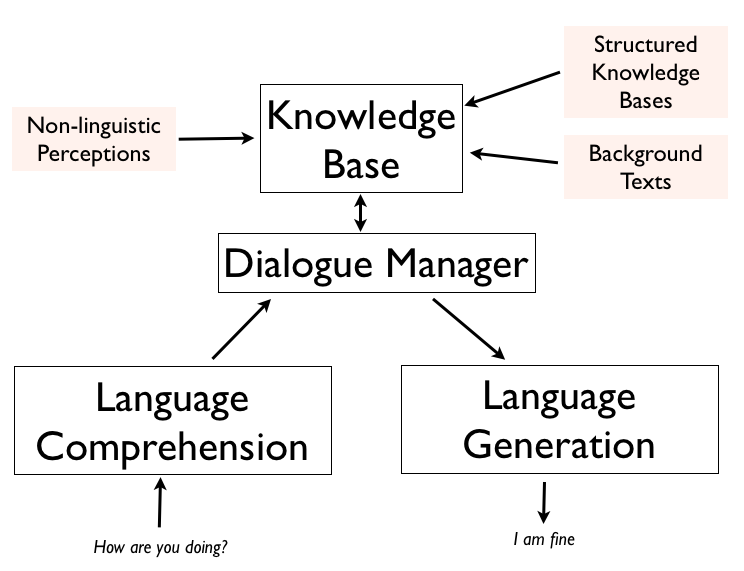
\includegraphics[width=12cm]{figures/dialogue_system.png}
\caption{ A generic dialogue-system architecture }
\label{fig:dialogue}
\end{figure}

总之,对话管理器全方位管理对话。它采用用户文本的语义表示、确定文本是否契合上下文,并构建系统响应的语义表示。一般来说,在它的职责中,以下几个是必要的:

\begin{itemize}
\item 保存对话历史
\item 采用一定的对话策略
\item 处理格式错误和无法识别的文本
\item 检索文件或数据库中的内容
\item 确保为使用者提供最好的响应
\item 管理启动和系统响应
\item 处理语言学问题
\item 言语分析
\item 以任何可用的、相关的非语言信息来构建语言结构。
\end{itemize}

目前大多数对话系统都利用一小部分固定规则来处理对话管理(这些规则代表人工制定的言语策略)。近年的一些系统还提供另一种方法:利用概率模型(如:POMDP)来控制对话,但这些系统还不具备有价值的实用性\cite{Young2006} \cite{Williams2010}。

\begin{figure}[htb]
\centering
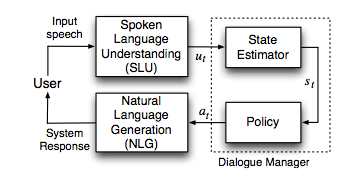
\includegraphics[width=12cm]{figures/pomdp.png}
\caption{ A POMDP-based reinforcement-learning-driven dialogue-system architecture }
\label{fig:dialogue}
\end{figure}


%%%%%%%%%%%%%%%%%%%%%%%%%%%%%%%%%%%%%%%%%%%%%%%%%%%%%%%%%%%%%%%
\subsection{言语行为论}{Speech Act Theory}
\label{sec:speechAct}
%%%%%%%%%%%%%%%%%%%%%%%%%%%%%%%%%%%%%%%%%%%%%%%%%%%%%%%%%%%%%%%

分析“对话系统”需要生成的各类话语的一个方法是:使用由Austin[?] 和 Searle [?] 开创,又经他人进一步完善的“言语行为论”。本文所阐述的对话研究中使用的正是这种方法。我们在这里先回顾非常基本的言语行为论,然后介绍言语行为论的具体变化。在研究过程中,我们发现这个理论是极有用的。

言语行为论的核心概念是:分析不连续言语行为的语言学行为,以实现特定的目标。在OpenCog环境下,这是一种使用方便的理论方法,因为它促使我们像对待OPenCog系统实施的其它行为一样对待言语行为,并推动我们通过标准的OpenCog行为选择机制来处理言语行为。
(图8)
“言语行为论”探讨那些可以通过言语来表现的行为类型。
	言表意的行为:某句话的外在表现,例如:真实言语和它的表面含义。
	言外行为:言语的“言外之力”,例如它的目标含义(作为社交层面的有效言语行为)。(按照Searle的使用方法,“言语行为”有时仅仅指的是言外行为。我们不用这个方法。)
	言后行为:它的实际效果,例如:说服、劝说、吓唬、启发、激励,或者让某人做或实现某个事项,不论是有意或无意的。在Searle看来,说话人通过他们的言语,只能获得5类言外之力,分别是:

	断言类:说话人自己承诺事情是真的。
The sky is blue (天是蓝色的)

	指令类:说话人试图让受话人做某事。
Clean your room! (打扫你的房间!)


	承诺类:说话人对未来的行为做出承诺。
I will do it (我将会做这件事)
	表达类:说话者表达了某些心理状态。
I’m Sorry (对不起)。
	声明类:说话人带来了不同的状况
The meeting is adjourned.(这个会议休会了)。

受这个本体论的启发,Twitchell 和 Nunamake在他们2004年的论文(标题为:言语行为归档:分析持续谈话和其参与者的概率统计法。[?])中提出了更加精细的“42种言语行为”本体论,叫做SWBD-DAMSL (DAMSL = Dialogue Act Markup in Several Layers)。尽管有少量不符合Searle的观点,并被分类为“其它”,但几乎他们所有的42种言语行为类型都能够被映射到Searle的5个高级类别之一。图??和??描述了这42种行为和它们与Searle分类之间的关系。我们已经利用了这个Searle解析法,它给我们正在进行的自然语言对话研究带来了灵感。

1.6.2 CogDial架构

在第??章的图??中,我们粗略地介绍了我们自己的对话架构。按照我们的方法,对话管理是通过一个通用动机认知模型来实施的,我们称之为“OpenPsi”。“知识”从我们的NL理解系统中分配到OpenCog的Atomspace知识存储中,然后OpenPsi会根据某一特定时间点的系统目标,从大量“言语行为模式”中选择一个,并用它来指导其余的宏观计划过程。随后,被选中的“言语行为模式”利用PLN推理和其它工具,实施认知处理,并收集知识组(例如:Atomspace中的原子、节点和链接),再将其分配到NL生成子系统中,以转换为英语。这个复杂的架构代表了人工编码和学习模块的融合。
 
(24和25页都是不需要翻译的图表)

\chapter{OpenCog AGI框架}{The OpenCog Artificial General Intelligence Architecture}

在本章我们将介绍通用人工智能体系结构OpenCog的一些关键技术。OpenCog是一个由多个子系统组成的庞大智能认知体系结构。更多有关此系统的技术,可以参考这本一千多页的书籍【XX】。在此我们只列出与本文研究紧密联系的几个关键的子系统,这样有助于理解本文的研究内容,包括前文中提到的自然语言理解、自然语言生成、逻辑推理以及智能会话系统建模等。
\section{ConPrime设计}{The CogPrime Design}

\indent OpenCog框架的核心是一个认知概念框架,称为CogPrime,但它们两者并不完全等同。OpenCog是一个更泛化的框架,用来实现许多特定AI程序以及可能的AGI设计。同时CogPrime可以单独被实现,而不要求被置于OpenCog框架中。一个在OpenCog中特别实现的CogPrime版本被称为OpenCogPrime。OpenCog是作为CogPrime的一个高效的、规划化的实现来设计的。

本节将概述CogPrime,它是一个实现AGI的概念和技术的框架,以一系列理论为基础。CogPrime的具体实现和测试(在OpenCog框架之内)仍然处在一个较浅的阶段,CogPrime的目标是表现出与人类智力性质接近的泛化智能,并最终可以被扩展到更广泛的领域的智能功能(?)。

CogPrime将在《Engineering General Intelligence》一书中有更详尽的描述[??],它将有超过1000页的篇幅,包括附录。本文的目标是以更紧凑的形式列举出其中一些关键点。在此我们略去CopPrime与其他已有的认知框架的比较,读者可以阅读以下文章[??],其中介绍了当前人工大脑与AGI构架的发展形式,其中包含了一个与较早版本的CogPrime框架的比较。

\subsection{认知协同:CogPrime的核心设计概念}{Cognitive Synergy: A Central Design Concept in OpenCog}
\indent CogPrime核心概念基础是以下三点:
\begin{itemize}
  \item 智能取决于系统的整体知识库中的特定高级结构和动力学的涌现;
  \item 我们尚未发现任何可以涌现出这类结构的算法或方案;
  \item 试图通过在一个系统内整合若干个不同的AI算法和框架来实现这种涌现的过程是微妙的,这些算法与框架的整合方式需要仔细地注意,而到目前为止这种整合并没有以正确的方式被执行。
\end{itemize}

人脑表现为许多不同的结构与动力学的整合,以通用的组件按照可感知的认知结构来组合到一起。然而,大脑的算法和结构被进化过程所影响,各部分紧密地联系在一起,互相适应,就像身体的不同器官之间的互相适应一样。这种协作使得整个系统表现出人类水平的泛化智能。我们相信,目前的AI中所缺少的部分是认知协同:不同组件的互相适应形成了整体恰当上的认知架构,在这个过程中,组件间以动态的方式充分地互相协作、彼此间紧密地相互联系在一起,就像人脑和身体的各部分一样,使得整体的架构和动力学涌现出来。这让我们得到CogPrime的核心假设之一:在一个恰当的认知框架和环境中,通过整合多重的符号和亚符号的学习和记忆组件,可以产生出与人类相当甚至更强的稳定的智能。

这类紧密的整合之所以尚未被充分探索,是因为它涉及到不同的层次,需要进行困难的框架和组件算法设计,这种设计应该保有某种面向架构和动力学的视角,使得它处在一个创造了合适的环境的系统中,以显现出架构和动力学。典型的,与不同的认知功能相对应的AI算法和架构已经通过各个研究者社区基于不同的理论规则进行了部署,并针对每个具体的运行环境进行的相应的性能调校。让这些性能迥异的组件共同工作在一起,并形成真正的协作是难以完成的任务。我们相信,以现有技术创造人类等级的AGI的“关键调料”,正是这种协同,而非一些特定的算法、结构、或架构原则。

\subsection{目前的和将来优先的OpenCog应用}{Current and Prior Applications of OpenCog}
为了更好地理解,到目前用来实现CogPrime的具体平台,我们将简略地讨论通过OpenCog系统实现CogPrime架构的部分工作。

OpenCog是一个开源的软件框架,以CogPrime架构的“OpenCogPrime”实现为目标(目前只是部分实现),已被用于自然语言处理和数据挖掘的商业应用。例如,参考[?]中OpenCogPrime的PLN推理以及RelEx语言处理被整合到一起,用来自动化地处理基于从PubMed中收集的信息的生物假设生成(?biological hypothesis generation)。[?]描述了使用OpenCog的MOSES组件进行生物信息分析;它的用途还被延伸到一些未被公开发表的商业应用中,例如财务预测、基因组、市场营销数据分析以及自然语言处理。在最近的相关工作中,OpenCog被用来控制虚拟世界中的虚拟代理[?]。
在2007-2008年间完成的原型工作涉及到使用一个叫OpenPetBrain的OpenCog的变形来控制虚拟世界中的狗。这些OpenCog控制的虚拟狗并没有表现出接近现实中狗的(或人类小孩)的智力,但它们展示了一系列有趣的相关功能,包括:
\begin{itemize}
  \item 基于模仿和强化来学习新的行为;
  \item 响应自然语言的命令和问题,作出恰当的行为和自然语言的回答;
  \item 自发地探索它们的世界,利用记忆来调整未来的学习和语言交互;
\end{itemize}

受游戏“我的世界”的启发,目前OpenCog正在将对虚拟狗的控制工作扩展到使用OpenCog控制游戏中的虚拟主体。这些主体最初被特别设定了各自在游戏世界中要达成的目标,为了完成这些目标,他们需要通过搬运“砖块”和使用简单的英语交流。这些任务可以是:

\begin{itemize}
\item 学习建造台阶或梯子来拿到高处的物体;
\item 学习建造掩体来躲避入侵者;
\item 学习建造环境中存在的类似结构物体
\item 学习建造桥梁以跨越峡谷。
\end{itemize}

当然,这一类任务中AI的显著性取决于系统能给予什么样的反馈、以及环境的复杂程度。让AI以非常独特的方式去做这些事情会相对简单,但这并非项目的主旨——目标是让系统通过涉身的经验以及少量的人类教师的反馈,学会使用泛化学习机制和泛化认知框架去完成类似任务。如果能成功,这将为今后的AGI研发提供一个非常不错的平台,就像一个可视化的和(immediately meaningful?)OpenCog的demo。

本文在写作时,项目团队的注意力集中在一些特定的任务上,包括:
\begin{itemize}
\item 观察另一主体通过建筑来到达高处的过程
\item 我们发现让虚拟主体观察另一个主体在一个不同的语境中,通过建造来到达高处的步骤,并模仿他的行为是一个不错的办法
\item 同时,如果虚拟主体需要一个特定的高处的物体,但是周围没有建造台阶所需的材料,那么尝试通过其他办法来达到高处(包括比如建造梯子或者让一个个子高的主体去帮他拿)
\item 我们发现,如果该主体需要隐藏自己有价值的物品,避免比自己更大的生物拿走它,那么他需要建造一个带有小洞的容器,这样该主体可以躲进去,但是比它大的生物无法进入。
\end{itemize}

延伸该工作到虚拟主体中,在2009-2010年间,预实验已经通过OpenCog在Nao机器人上进行过了[?]。这些涉及到将OpenCog与一个分离的控制底层感知和行动的子系统的整合。这个整合仅通过相当简单的方式进行,然而,如何进行该整合是论文[?]和[?]中讨论的话题,本文仅仅介绍到此。在此方面的工作在2013-2015年间一直在进行中,由Hong Kong Innovation in Technology Fund的一个基金赞助。

\subsection{概念背景}{Conceptual Background}
\indent CogPrime的设计研发受到一种叫“模式主义”的心灵哲学影响[?]。模式主义心灵哲学是对如何实现智能系统的统筹思考。它基于一个简单的前提,即心灵由模式组成——同时心灵是一个对它自己和世界的模式识别系统,尤其是那些关于在何种语境下、何种过程会导致何种结果的模式。然而,CogPrime受模式主义视角的指引这一点不应被过分解读。CogPrime是一个集成设计,通过若干不同的哲学、科学以及工程的想法的结合来形成,它的成功或失败并不取决于某一特定的哲学对智能的理解。

在细节上,追寻模式主义哲学会导致一系列特定的关于心灵本质的假设和结论。通过智能在复杂环境中完成复杂行为,我们发现一个认知系统的动力学会被一下两种因素影响:
\begin{itemize}
\item 自组织,通过系统动力学引起退出系统的模式来产生一个新的(???);
\item 面向目标的行为,在[?]中有严格的定义,但基本上相当于一个与环境交互的系统,该系统的行为类似于求某些可理解的简单函数的最大值。
\end{itemize}

自组织和面向目标行为应该被理解为互相协作的两个方面。举一个详细的例子,一个虚拟主体被要求通过一些砖块建造一个惊人的建筑,这是面向目标的。但是该主体如果在之前有过在自法的、无结构性的玩耍砖块的过程,那么它能更好地完成该面向目标的任务。同时这种要求它建造一个惊人的砖块结构的“创造力的推动”可能引起它去探索,以得到一些新奇的模式,而它可能将这些模式重新用于将来的非结构性的砖块游戏中。

基于以上概念,如[?]中所讨论的,我们可以假定若干主要的动力学原则,包括:
\begin{itemize}
\item 演化,作为一个主要过程,通过它,可以在很大数量的模式中挑选出一些,用于形成新模式的基础,基于一些与主体所要完成的任务相关的“适应度函数”;
\item 自生成:该过程让拥有多个模式交互的系统维持它的整体性,当系统中的一个模式开始降低其强度(?Intensity)时,一些其他的模式会增加他们的强度,以使得该遇到麻烦的模式重新开始增加它的强度;
\item 联系,给予注意力的模式,会将注意力散布一部分在其他曾经有过联系模式上。同时,根据皮尔斯的心灵定律[?],简述之,即心灵是一个互相联系的记忆网络,它的机制是,记忆中的每一个想法都是一个激活的智能体(agent),这个网络持续地与那些和它有关联的记忆发生作用 ;
\item 差别的注意力分配;评分系统。那些被评价为对达成目标更有价值的模式会被给予更多的注意力,并被鼓励参与新模式的生成;
\item 模式创造,被井架为对实现目标更有价值的的模式被变异与组合来产生新的模式。
\end{itemize}

接下来,按照[?]中列出的许多理由,我们假定智能系统中的模式网络必然引起一下大规模产生的结构
\begin{itemize}
\item 层次化网络。模式被与控制其他代表了更特化方面的模式所联系起来。
\item heterarchical网络(?)。系统维持一个关于那些曾经与其他模式相联系的模式的记忆。
\item 双网络。这两种结构被合并,通过一种机制让它们和谐共处。通过许多可能的方式,层次化地组织起一批模式,并保证层次结构中接近的模式有更多通向彼此的有意义的heterarchical连接;当然,必须有一个在层次结构中接近的模式间搜索heterarchical连接的机制。
\item 自结构。网络中模式的一部分形成了整个网络的结构的大致的图景。
\end{itemize}

CogPrime并没非直接由这些哲学规则产生;它最初通过合并人类认知心理学和计算机科学算法结构而创建,然后修改这个组合以产生一个系统,使它看起来与这些哲学规则相一致的、并且以当前的硬件基础在计算上可行,它还将包括一个大致上与人类相似的认知结构。CogPrime的成功将主要取决于这些高阶结构和机制是否能够通过CogPrime中表达和算法的系统交互中产生出来,它们将被用于在恰当的环境中控制恰当的主体。在[?]中详细讨论了这些抽象的概念如何从CogPrime的结构和算法中具体地产生出来。

\subsection{CogPrime的高阶架构}{High-Level Architecture of OpenCog}

图\ref{fig:CogPrime1}描述了CogPrime的高阶架构。一个关键的潜在原则是:与多种类型的记忆相联系的多认知过程的运用,将会使得一个智能主体执行它认为在当前环境下对完成目标最有利的过程。例如,在机器人学龄前阶段的条件下,最高层的目标将会是日常的事物,如取悦老师、学习新的知识和技能、保护机器人的身体。

将这些图表与人类的认知结构图表进行对比是有趣的\cite{Goertzel2012a},它将概述目前所理解的人类认知结构。二者主要的区别在于,CogPrime的图表用于特定的结构(如知识表征)和过程,然而泛化的整合性图表架构仅仅只涉及结构和过程。举例来说,整合图表涉及陈述性知识和学习,然而CogPrime图表指的是PLN,一个关于陈述性知识的推理和学习的特定系统。在\cite{Goertzel2010a}中用一个表格来表示CogPrime图表和以整合图表表示的人类认知结构、过程之间的联系,这表示了被每个CogPrime组件所实例化泛化的认知功能。

\begin{figure*}[htb]
\centering
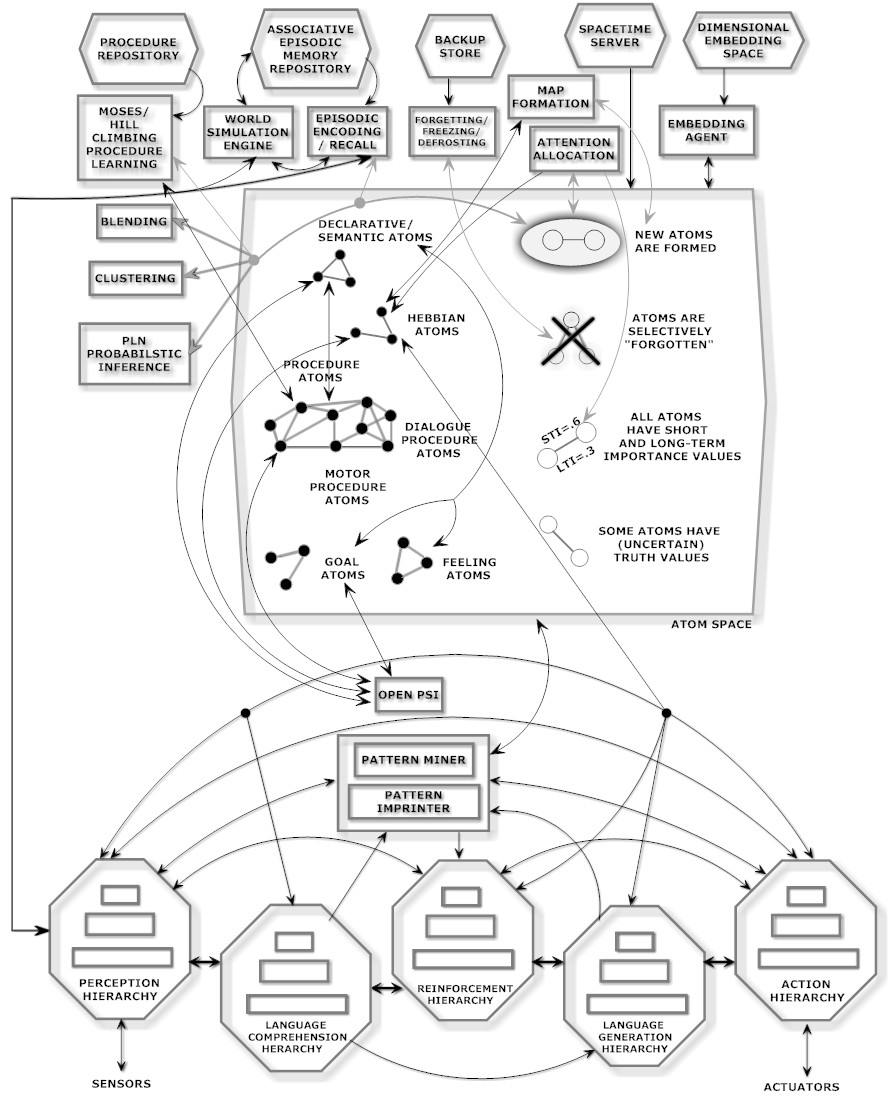
\includegraphics[width=14cm]{figures/1.jpg}
\caption{ {\bf High-Level Architecture of OpenCog.}  This is a conceptual depiction, not a detailed flowchart (which would be too complex for a single image).   }
\label{fig:CogPrime1}
\end{figure*}

\subsection{表征和记忆}{Representation and Memory}

\paragraph{本地和全局知识表征}

OpenCog的知识表征机制在根本上是基于{\it 网络}的。把精神当作网络的观点是隐含在模式主义哲学中的,因为每一个模式都可以被看成某物的模式,或关于某物的布置的模式——因而一个模式总是可以被看做二个或更多物体之间的关系。一系列的模式形成一个模式网络。各类知识可以以网络形式来表达,而认知过程也可以被表达为网络,举例来说将它们表达为程序,以各种树或图的形式表达。在一个智能中模式的涌现可以 被看作自身的一个模式网络;在涉身的心灵和它的物理和社会环境之间的关系可以被看做某种生态和社会网络。

知识表达系统的两个主要超类是{\it 局部}(也被称为{\it 显示})和全局(也被称为{\it 隐式})系统,我们用一个被称为{\it 全局-局部}的混合类包含了这两者。在一个{\it 局部}系统中,每一条知识都是用一小部分认知系统的元素来存储的;在一个{\it 全局}系统中,每一条知识都被以一种特定的模式存储与激活,比如以认知系统的一定比例的元素的形式;在一个{\it 全局-局部}混合系统中,这两种方式被共同使用。以上三种知识表征类型都可以被网络所实现。在CogPrime中,这三者都是以{\it 同样}的网络(Atomspace)来实现。

\paragraph{CogPrime中的记忆类型和相关认知处理}

CogPrime依靠多种的记忆类型,如同上面所讨论的,它的前提是正确地建立一个类人AGI系统,以处理不同类型的记忆,这些记忆包括了结构和动力学。

CogPrime的记忆类型有:陈述性记忆、过程性记忆、感知记忆、以及场景记忆,这些在认知科学中被广泛讨论\cite{Tulving2005}的记忆类型,以及分配泛用的系统资源的注意力记忆、和为特定目标分配系统资源的意向性记忆。表格\ref{tab:opencog}概述了这些记忆类型,给出了关键的引用并指出了相关的认知过程,同时指出了每一个认知过程(模式创造、联系等)所对应的泛化的模式主义认知动力学。

以模式主义认知理论的形式,CogPrime中的多种记忆类型可被看做特定类型模式的特化存储方式,并经过了计算时间与空间上的优化。联系到某种特定类型的记忆的认知过程被用来创造和识别该记忆的类型。原则上所有类型的模式都可以在统一的记忆和处理构架下进行,CogPrime所用到的这种类型特例化,是为了能够在现有的计算条件可接受的前提下创造有效的泛化智能。我们在\cite{Goertzel2010c}中所详细论述过,高效性并不是可有可无的,而是对真实世界中的泛化智能举足轻重的特性(就像Hutter所展示的,如果没有效率的限制,任意登记的泛化智能都可以通过简单而琐碎的程序来实现)。

CogPrime设计的本质在于,与每种类型的记忆相关的数据结构和处理过程是被紧密联系在一起的,相比于仅仅包含同一种结构和处理过程的而仅仅以不同的黑盒分割开的构架,它产生了协同性的智能。

OpenCog中设计有交互的认知处理过程,以使得不同类型的记忆间可以互相转换,尽管有时这会消费较多的计算资源(比如,一段陈述性的知识可能通过一些努力被解释为过程性或场景性的知识);同时,对于一个主要处理某一种类型记忆的学习进程来说,它可能会经常通过把知识转换成其他类型来解决问题,比如认知协同任务。

\newcolumntype{Y}[1]{>{\centering\hspace{0pt}\arraybackslash}m{#1}}

\begin{table*}[ht]
\centering
\begin{tabular}{|Y{3cm}|Y{5cm}|Y{3cm}|}
\hline \textbf{记忆类型} & \textbf{特定的认知过程} & {\bf 泛化的认知功能} \\ \hline
\textbf{陈述性} & 概率逻辑网络PLN\cite{Goertzel2008}; 概念调整\cite{Fauconnier2002} & 模式创造 \\ \hline
\textbf{过程性} & MOSES(一个创新的概率演化运算学习算法)\cite{Looks2006} & 模式创造 \\ \hline
\textbf{场景性} & 内部模拟引擎\cite{Goertzel2008d} & 联系,模式创造 \\ \hline
\textbf{注意性} & 经济注意力网络(ECAN)\cite{Goertzel2010} & 联系,评分 \\ \hline
\textbf{意向性} & 概率目标层次按照OpenPsi动机框架通过PLN和ECAN来细化\cite{Bach2009}) & 评分,模式创造 \\ \hline
\textbf{感知} & 在CogBot中通过DeSTIN组件来支持 & 联系,注意力分配,模式创造,评分 \\ \hline
\end{tabular}%
\caption{CogPrime中的记忆类型和认知处理过程。第三列表示每一个特定的认知处理过程所拥有的泛化认知功能,它们给予认知的模式主义理论.}
\label{tab:opencog} 
\end{table*}

%%%%%%%%%%%%%%%%%%%%%%%%%%%%%%%%%%%%%%%%%%%%%%%%%%%%%%%%%%%%%%%
\section{OpenCog中AtomSpace的表示形式}{OpenCog AtomSpace Representation}
\label{sec:atoms}
%%%%%%%%%%%%%%%%%%%%%%%%%%%%%%%%%%%%%%%%%%%%%%%%%%%%%%%%%%%%%%%

XXXX备用:其基本的存储单元称为“原子”(Atom)。每一个Atom携带的值(Value)的结
构为(STI,LTI,TruthValue,Confidence,Content)。STI(Short Term Importance)
和LTI(Long Term Importance)可以用来模拟短期记忆(Short Term Memory)和长期
记忆(Long Term Memory)。XXXX

正如上述所言,Atomspace是OpenCog中所使用统一且通用的知识库,它使用包含特定类型的节点(Node)和链接(Link)的加权有向超图结构来表示知识,主要用作表示叙述性的知识,同时亦间接地表示其它类型的知识。这些特定类型的节点和链接是经过包括语义层面的细心挑选,以满足OpenCog在认知过程的需要。由于OpenCog的Atomspace表示形式是本文的核心,在这里我们会详细列出几个简单的示例予以说明。

以下是一个以OpenCog常用的表示方法去表示OpenCog中的链接的例子:
 
{\tt\begin{small}\begin{lstlisting}
InheritanceLink Lian_Ruiting animal <.99>
\end{lstlisting}\end{small}}

\noindent 或更明确地:

 {\tt\begin{small}\begin{lstlisting}
InheritanceLink <.99>
	ConceptNode "Lian_Ruiting"
	ConceptNode "animal "
\end{lstlisting}\end{small}}

以及:

{\tt\begin{small}\begin{lstlisting}
EvaluationLink <.7>
	chase 
	ListLink
		cat
		mouse
\end{lstlisting}\end{small}}

\noindent 或更明确地:

{\tt\begin{small}\begin{lstlisting}
EvaluationLink <.7>
	PredicateNode "chase" 
	ListLink
		ConceptNode "cat"
		ConceptNode "mouse"
\end{lstlisting}\end{small}}

\noindent 正如上述示例所示,节点通常具有名称,而链接则没有,但链接可以连接一个或多个的目标,而这些目标可以是节点或链接。

综合来说,Atomspace是一个“带标记的通用超图“,这些标记可以是节点的名称或其真值等等。“超图“与一般“图“的其中一个主要不同之处在于其链接,例如ListLink或SetLink,它是可以连结两个以上的参数,而其通用性也允许这些链接与其他的链接相连,而不只局限于节点。

另一个值得注意的地方是这些节点的名称,虽然在这些示例中它们都是以英语来表示,但实际上OpenCog会在日常操作中透过自主学习去创造一些新的节点,而这些节点往往都不会和我们的语言概念相对应。

更重要的一点是, AtomSpace的知识表示形式的主要功能是提供一个灵活的方式去紧凑地表达多种相关形式的知识,并允许它们之间有交互操作。其中的“交互操作“是指,例如,一组的陈述性的知识可以跟另一组的注意力相关或程序性相关的知识相互连结,或一组在一个类别的知识可以跟另一组在其他类别的知识重叠在一起(同一链接同时有著一个陈述性相关的真值和一个注意力相关的重要值)。总而言之,只要有任何表示形式能够提供足够的灵活性来:

\begin{itemize}
\item 紧凑地表达所有在人类记忆中扮演著主导角色关键类别
\item 灵活地创建特定的副表示形式去表达在上述这些关键类别中的知识,同时又能够被迅速地改动或操纵这些知识
\item 重叠和连结不同种类的知识,包括上述这些特定的副表示形式
\end{itemize}

\noindent 以上几项都符合OpenCog的整体要求。而这些Atom的表示形式已能满足此计设的总体要求,并从软件的角度来看已证明是可行的。

\subsection{基本的Atom种类}{Basic Atom Types}

在OpenCog中最基本而且经常会用到的Atom种类中的节点是:

\begin{itemize}
\item ConceptNode -- 表达任何的单元,具体或抽象但又不能以其他特定的节点种类来表达的概念
\item PredicateNode  -- 表达一个为Atom产生真值的程序(以下会有详细说明)
\item SchemaNode -- 表达一个以一个Atom产生另一个Atom的程序,或产生一些其他效果
\end{itemize}

和以下的链接:

\begin{itemize}
\item MemberLink -- 连结一个通用种类的Atom和一个ConceptNode,并拥有一个模糊真值
\item InheritanceLink -- 连结两个ConceptNodes,并拥有一个概率真值
\item SimilarityLink -- 连结两个ConceptNodes,并拥有一个概率真值
\item EvaluationLink -- 连结一个PredicateNode以及其参数
\item ExecutionLink -- 连结一个SchemaNode、其需要的参数以及其产生的输出
\begin{itemize}
\item ExecutionOutputLink -- 连结一个SchemaNode以及其输入,当遇到特定的认知程序时才会产生输出
\end{itemize}
\end{itemize}


\subsection{绑定程序的节点}{Grounded Procedure Nodes}

SchemaNode和PredicateNode有两种形态:已绑定和未绑定。未绑定是指系统尚未知道应该如何评定该方案,或系统将会以一连串的ExecutionOutputLinks来绑定该方案。而已绑定的会有一个特定程序的名称(目前该程序可以是C++,Scheme或Python语言编写的程序)来执行该方案。例如:

\begin{verbatim}
ExecutionOutputLink
	GroundedSchemaNode "plus.py"
	ListLink
		NumberNode "2"
		NumberNode "3"
\end{verbatim}

\noindent 当执行时,会调用Python函数“plus“来把“2“和“3“加起来,然后产生一个名为“5“的NumberNode作为其输出。

\subsection{內涵与外延的关系}{Intensional and Extensional Relationships}


OpenCog的链接类型中亦有多种拥有继承和相似性质的链接,例如IntensionalInheritanceLink和ExtensionalInheritanceLink,其细节将会在\cite{PLN}中详述,但简而言之,以下链接的真值:

\begin{verbatim}
ExtensionalInheritanceLink A B
\end{verbatim}

\noindent 同时亦可被表示为:

\begin{verbatim}
SubsetLink A B
\end{verbatim}

\noindent 是一个条件概率$P(B|A)$。另一方面,以下链接的真值:

\begin{verbatim}
ExtensionalInheritanceLink A B
\end{verbatim}

\noindent 是一个条件概率$P(prop(B)|prop(A))$,当中$prop(X)$表示在PLN推理系统中定义的模糊集合X的属性。

\subsection{SatisfyingSet}{SatisfyingSet}
SatisfyingSet的算符能够表达一个集合关系的概念,而当中每一位成员都是乎合同一个述语的元素,并用Member的关係形式,以一个模糊数值(而非概率数值)来表达该元素属于一个概念的真确性。

举例来说,假设现在有“FriendOfBob“这个述语和三个元素“Jack“、“John“和“Jill“:

\begin{verbatim}
Evaluation <.7>
	FriendOfBob
	Jack

Evaluation <.6>
	FriendOfBob
	John

Evaluation <.8>
	FriendOfBob
	Jill
\end{verbatim}

根据SatisfyingSet算符的定义,我们会得出以下的Member:

\begin{verbatim}
Member <.7>
	Jack
	SatisfyingSet
		FriendOfBob

Member <.6>
	John
	SatisfyingSet
		FriendOfBob

Member <.8>
	Jill
	SatisfyingSet
		FriendOfBob
\end{verbatim}

\subsection{等效式与启示式}{Equivalence and Implication}

现在我们可以为述语定义等效式与启示式,如同为概念定义相似式和继承式一样:

\begin{verbatim}
Equivalence
        A
        B
\end{verbatim}

是等同于:

\begin{verbatim}
Similarity
        SatisfyingSet(A)
        SatisfyingSet(B)
\end{verbatim}

以及:

\begin{verbatim}
Implication
        A
        B
\end{verbatim}

是等同于:

\begin{verbatim}
Inheritance
        SatisfyingSet(A)
        SatisfyingSet(B)
\end{verbatim}

以上是混合了等效式与启示式的表达形式。内涵与外延的表达形式都是以类似的方式去表达,以下是一个ExtensionalEquivalence的例子:

\begin{verbatim}
ExtensionalEquivalence
        A
        B
\end{verbatim}

是等同于:

\begin{verbatim}
ExtensionalSimilarity
        SatisfyingSet(A)
        SatisfyingSet(B)
\end{verbatim}

\subsection{Boolean链接}{Boolean Links}

Boolean链接是用来表达一些常用操作的概率:ANDLink、OrLink、NOTLink和XORLink。

同时,就像其他编程语言般,Atomspace亦有“IfElseLink“以作为一个判断选择的条件简写:

\begin{verbatim}
ElseLink
	R
		A
		B
	C
\end{verbatim}

是等同于:

\begin{verbatim}
AND
	R
		A
		B
	R
		NotLink
			A
		C
\end{verbatim}

\noindent 这个设计能有效防止产生过多的链接种类,例如IfImplicationElse、IfExtensionalImplicationElse、IfIntensionalImplicationElse、IfInheritanceElse等等。
	
		
\subsection{真值}{Truth Values}
\label{真值}

一个Atom的真值是用来表示一个Atom的\textit{真确性},在某程度上是取决于Atom的类型。这个数值是以一个TruthValue物件的形式跟Atom链接在一起。一般来说我们会在Atom的表示式后以\ensuremath{<}\ensuremath{>}及一个数字来显示其真值,例如:

\begin{verbatim}
A <.4>
\end{verbatim}

來表示一個名稱为“A“的Atom的真值为.4。同样地:

\begin{verbatim}
IntensionalInheritanceLink Ben monster <.5,.9>
\end{verbatim}

\noindent 来表示一个连接著“Ben“和“monster“的IntensionalInheritance关係中有著一个.5的强度和.9确信情度。总而言之,\ensuremath{<}tv\ensuremath{>}表示著一个平均值为tv的概率分佈。这些概念和语义将会在\cite{PLN}中作详细展述。

\subsection{量词}{Quantifiers}  

在不明确逻辑理论中,量化过程是一个比较细微的事项。PLN包含了标準的ForAll和ThereExists的量词(使用高阶概率定义的概率真值),在处理量化过程时主要会用AverageQuantifier来建构,例如:

\begin{verbatim}
AverageQuantifier $X
        F($X)
\end{verbatim}

的真值为F(\$X)的真值的加权平均值,即是以下的总和:

\begin{verbatim}
w($X) F($X) / N
\end{verbatim}

\subsection{总结——语言相关的Atom类型}{Summary of Language-Relevant Atom Types}

接下来将会描述一些用来表达具体语言概念的Atom类型。

原则上,要处理从ASCII编译的语言资料,除了需要CogPrime结构外就只有以下两个节点类型和一个链接类型:

\begin{itemize}
\item CharacterNode
\item CharacterInstanceNode
\item ListLink
\end{itemize}

\noindent 因而字串就可以以列表或拼接的方式来表达,例如“pig“可以以列表$(\#p, \#i, \#g)$来表达。

然而,实际上定义特定的語言Atom类型也很有帮助的,例如:

\begin{itemize}
\item	MorphemeNode/ MorphemeInstanceNode
\item		WordNode/WordInstanceNode
\item		PhraseNode/PhraseInstanceNode
\item		SentenceNode/ SentenceInstanceNode
\item		UtteranceNode/ UtteranceInstanceNode
\end{itemize}





\subsection{基于类型理论的Atomspace形式化表示}{A Formal Type System for OpenCog’s Atomspace}

引入Atomspace的形式化表示能容许我们在不用关注输入是否完全正确的情况下精密地应用Atomspace,并能在某些情况下减少制造混乱的同时又提高系统的精确度。为实现这目的,我们建立了一个基于类型理论的形式化表示机制,具体来说,我们采用了Haskell的泛代数数据类型 \cite{Haskell2014}对Atomspace形式化如下:

\begin{verbatim}
data TV = SimpleTV Float Float

data ConceptName = ConceptName String

data VariableName = VariableName String

data Atom a where
	-- TV
	TV :: TV -> Atom TV
	TVAnd :: Atom TV -> Atom TV -> Atom TV
	TVOr :: Atom TV -> Atom TV -> Atom TV
	TVGetTV :: Atom a -> Atom TV

	-- Predicate
	Predicate :: (Atom a -> TV) -> Atom (Atom a -> TV)
	PredicateAnd :: (a ~ (Atom b -> TV)) => Atom a -> Atom a -> Atom a
	PredicateOr :: (a ~ (Atom b -> TV)) => Atom a -> Atom a -> Atom a
	Implication :: (a ~ (Atom b -> TV)) => Atom a -> Atom a -> Atom TV
	Equivalence :: (a ~ (Atom b -> TV)) => Atom a -> Atom a -> Atom TV
	Evaluation :: (Atom (Atom a -> TV)) -> Atom a -> Atom TV

	-- Concept
	Concept :: ConceptName -> Atom ConceptName
	ConceptAnd :: Atom ConceptName -> Atom ConceptName -> Atom ConceptName
	ConceptOr :: Atom ConceptName -> Atom ConceptName -> Atom ConceptName
	Inheritance :: Atom ConceptName -> Atom ConceptName -> Atom TV
	Similarity :: Atom ConceptName -> Atom ConceptName -> Atom TV
	Member :: Atom a -> Atom ConceptName -> Atom TV
	SatisfyingSet :: Atom (Atom a -> TV) -> Atom ConceptName
	
	-- Variable
	PredicateVariable :: VariableName -> Atom (Atom a -> TV)
	ConceptVariable :: VariableName -> Atom ConceptName
	TVVariable :: VariableName -> Atom TV
	Variable :: VariableName -> Atom a

	-- Binding
	Bind :: Atom a -> Atom TV -> Atom (Atom a -> TV)

	-- Quantifier
	ForAll :: Atom a -> Atom TV -> Atom TV
	Exists :: Atom a -> Atom TV -> Atom TV

	-- number
	Number :: (Num a) => a -> Atom a

	-- Schema
	Schema :: (a ~ (Atom b -> Atom c)) => a -> Atom a
	ExecutionOutput :: (a ~ (Atom b -> Atom c)) => Atom a -> Atom b -> Atom c

	-- List
	List :: [Atom a] -> Atom [Atom a]
\end{verbatim}	

以下是一些使用该形式化机制表示Atomspace超图的例子:

\begin{verbatim}
-- Functions from Atom to TV to build predicates
is_bottom :: Atom a -> TV
is_bottom = undefined
is_top :: Atom a -> TV
is_top = undefined
is_car :: Atom a -> TV
is_car = undefined

-- And/Or hypergraph of concepts
a = Concept (ConceptName "A")
b = Concept (ConceptName "B")
c = Concept (ConceptName "C")
h1 = ConceptOr (ConceptAnd a b) c

-- And/Or hypergraph of predicates
h2 = PredicateOr (PredicateAnd (Predicate is_top) (Predicate is_car)) (Predicate is_bottom)

-- Apply Evaluation to predicate h2
tv3 = Evaluation h2 (List [Concept (ConceptName "BMW")])

-- Build a Schema
add :: (Atom [Atom Float]) -> Atom Float
add (List [Number x, Number y]) = Number (x + y)
add _ = undefined
h4 = Schema add -- :: Atom (Atom [Atom Float] -> Atom Float)

-- Apply a Schema
h5 = ExecutionOutput h4 (List [Number 3, Number 4]) -- h5 :: Atom Float

-- Test GetTVLink
tv1 = TVGetTV h1
tv2 = TVGetTV h2

-- Test AndLink with TV
tv4 = TVAnd tv1 tv3
\end{verbatim}	

%%%%%%%%%%%%%%%%%%%%%%%%%%%%%%%%%%%%%%%%%%%%%%%%%%%%%%%%%%%%%%%
\section{OpenCog的模式匹配器Patter Matcher}{The OpenCog Pattern Matcher}
%%%%%%%%%%%%%%%%%%%%%%%%%%%%%%%%%%%%%%%%%%%%%%%%%%%%%%%%%%%%%%%

其中一个在OpenCog语言处理中最常使用的工具是一个模式匹配器。OpenCog的模式匹配器是一个查询引擎或变数配对者,主要功用是在Atomspace中寻找特定的模式,或是一些Atom相关排列或“模板“。在轮入一个等定的Atom排列(即一个超图)后,模式匹配器会从Atomspace中寻找所有合乎条件的超图。同时一些“空白位置“,即“变数“在一个超图的位置,亦可存在于该输入的超图当中,而模式匹配器则会“填补“这些“空白位置“。例如:“John threw a \_\_\_\_).“亦可以被判断为“John threw a ball.“,前提是在查询前该句子要存在于Atomspace里,而在这个例子中“ball“就是被配对的一个答案。输入的超图中可以在不同的地方拥有多过一个的“空白位置“,同时亦可以有多过一个的答案。在这过程中,BindLink提供了一个便利的API去达到这目的,接下来会有更多的技术层面说明。

模式匹配器是一个变数配对者,是在传统计算机科学中“统一“的概念,因为这是它的功能之一。它同时亦是一个查询引擎,因为这个变数配对过程某情度上是等同于用SQL在关联数据库中进行查询。当中主要的分别在于在OpenCog中概念是以超图的形式表示,所以它亦可以被形容为一个超图查询语言HQL(Hypergraph Query Language)。但这些都只是以不同的名称去表示同一个程序。

这个模式匹配器亦是结构精密应用的一个重要组件,同时亦是建立前向和后向链接的一个重要基础。它拥有C++和Scheme的接口以供不同的应用。

模式匹配器是由数个不同的组件连接在一起,组成一个基础前向链接或超图重写的工具。在其核心是一个能比较和配对不同超图以及其变数的组件,而这个组件跟另一个“找寻器“一同使用便能寻找整个Atomspace中的合乎条件的超图。最后一个组件是一个“编写器“,主要功用是当有一个配对成功产生后建立一个或以上在ImplicationLink后半部列明的超图。

这个模式匹配器接受有指定“规则“的BindLinks,再把这些“规则“应用到Atomspace里。每一个“规则“是一个ImplicationLink,以“if P then Q“的形式表达,当中P和Q分别代表不同的超图。如果P被实现了,那么便能得到Q。Q可以是任何种类的超图,但如果Q是一个ExecutionLink,这便意味著当P被实现了,系统便将会实行其他程序,这在整体来说可以是一个十分强大的功能,因为在一般情况下很多程序都可以以ExecutionLink来执行。

模式匹配器不会更改任何超图中的真值(Truth Value)或关注值(Attention Value),有需要时使用者亦可以自行编写和执行相关的程序。

在默认的回调函数中模式匹配器会搜索整个Atomspace,因此亦有需要编写特定的回调函数以限制其搜索范围,例如只寻找和接受拥有某程度短期重要性的Atom,以只获取相对重要的资讯。

以下是一个使用模式匹配器的示例:

\begin{verbatim}
(define find-animals
  (BindLink
    ;; The variable to be bound
    (VariableNode "$var")
    (ImplicationLink
      ;; The pattern to be searched for
      (InheritanceLink
         (VariableNode "$var")
         (ConceptNode "animal")
      )
 
      ;; The value to be returned.
      (VariableNode "$var")
    )
  )
)
 \end{verbatim}
 
只要在OpenCog Scheme shell中输入以下指令便能执行以上的模式匹配器以找出在Atomspace中所有继承“animal“的概念:

\begin{verbatim}
(cog-bind find-animals)
\end{verbatim}


%%%%%%%%%%%%%%%%%%%%%%%%%%%%%%%%%%%%%%%%%%%%%%%%%%%%%%%%%%%%%%%
\section{概率逻辑网络PLN}{Probabilistic Logic Networks}
\label{sec:pln}
%%%%%%%%%%%%%%%%%%%%%%%%%%%%%%%%%%%%%%%%%%%%%%%%%%%%%%%%%%%%%%%

概率逻辑网络PLN是OpenCog的一个很特殊的方面,在此文中它讲被重点提出,尤其在第\ref{chap:inference}章,PLN是一个独特的推理系统,它嵌入了预测逻辑和传统逻辑的组合。PLN在\cite{Goertzel2008, RWR}中被详细介绍。在此我们给出一个高阶的概述。

PLN是一个数学和软件框架,用于非确定推理、操作CogPrime软件框架、使概率真值与泛化逻辑推理规则的整合成为可能。具体来说,PLN包含:

\begin{itemize}
\item 一系列推理规则(例如,演绎、贝叶斯规则、变量归一化、演绎推理,等等),每一项都有一个或多个逻辑关系或词项(以CogPrime的原子来表征)作为输入,并计算输出;
\item 特定的数学方程,基于合适的背景前提假设的概率值,计算结论的概率值。
\end{itemize}
PLN还涉及一条特殊的功能,评估概率值的置信度(证据的分量,或二阶的不确定性)。最后,PLN在软件中的实现需要重要的抉择,要求考虑推理规则的结构化表征、“推理控制”——这种策略要求,在每个特定的实际情况中,判断以何种顺序做何种推理。

\subsection{PLN的一个简单概述}{A Simple Overview of PLN}

PLN的关键因素是它的规则和方程式。总的来说,一个PLN规则有:

\begin{itemize}
\item 输入:一个原子元组(它必须满足某些要求,视规则而定)
\item 输出:一个原子元组
\end{itemize}

实际上,几乎在所有情况下,输出都是一个单一的原子,而输入则是一个单一的原子或者是一对原子。

特定的原形例子是演绎规则,它的输入是这样的:

{\tt\begin{small}\begin{lstlisting}
X_Link A B
X_Link B C
\end{lstlisting}\end{small}}

而它的输出应该是这样的:

{\tt\begin{small}\begin{lstlisting}
X_Link A C
\end{lstlisting}\end{small}}

在这里,X\_Link可以是继承性链接、子集链接、按时链接或延伸按时链接的。

一个PLN方程与一条PLN规则同时存在,它表示了输出的非确定性真值,基于输入的非确定真值。例如,如果我们有:

{\tt\begin{small}\begin{lstlisting}
X_Link A B <sAB>
X_Link B C <sBC>
\end{lstlisting}\end{small}}



那么标准的PLN演绎方程告诉我们

{\tt\begin{small}\begin{lstlisting}
X_Link A C <sAC>
\end{lstlisting}\end{small}}

其中: 

$$
s_{AC}=s_{AB}s_{BC}+\frac{\left(1-s_{AB}\right)\left(s_C-s_Bs_{BC}\right)}{1-s_B}
$$, $s_A$表示节点$A$的真值强度。

在这个例子中,每一个院子的非确定真值通过一个“强度”数值来给出。总的来说,PLN中的非确定真值可以有多种形式,比如:

\begin{itemize}
\item 单一的强度值,比如0.8,这表示概率或模糊真值,取决于具体的原子类型
\item (强度,置信度)对,比如(0.8,0.4)
\item (强度,数量)对,如(0.8,15)
\item 非确定的概率值,如(0.6,0.9, 0.95),这表示概率间的相互评分
\end{itemize}

\subsection{前向和后向链}{Forward and Backward Chaining}

PLN中典型的模式的使用是前向链和后向链推理。

前向链表示:

\begin{enumerate}
\item 给出一个感兴趣的原子池(列表);
\item 应用PLN规则到这些原子上,以产生新的原子,最好也是感兴趣的;
\item 将这些新的原子加如到池中,返回步骤1。
\end{enumerate}

例子:“人是动物”和“动物会吸”是两个池中的原子。它们被演绎规则所组合,形成了结论“人会呼吸”

后向链分为两种情况,第一种:

\begin{itemize}
\item “真值查询”,给出一个原子目标,它的真值未知(或者过于不确定),以及一个原子池,按照演绎规则,通过组合池中原子,找到一种方法来评估该目标原子的真值。
\end{itemize}

例子:目标是“人是否会呼吸?”(继承链接“人会呼吸”)。目标的真值通过“人是动物,动物会呼吸,因此人会呼吸”的推理来评估。

第二种:

\begin{itemize}
\item “填空查询”,给定一个目标链接(原子可以是节点或链接)以及一个或多个目标中间的变量原子,找出什么原子可以被放在变量原子的位置上,可以使目标链接获得一个高的置信度(即一个“高的真值”)。
\end{itemize}

例子:目标是“什么会呼吸”,即“继承链接\$X呼吸”……直接在原子空间中查找发现院子“继承链接 动物会呼吸”,表示空格\$X的位置上可以被填入“动物”。推理揭示“继承链接 人会呼吸”,因此空格\$X也可以被填入“人”。

例子:目标是“什么会呼吸和加法”,即“(继承链接\$X会呼吸)并且(继承链接\$X会加法)”。推理揭示此处\$X可以被填入“人”但不能是“猫”或“电脑”。

常识推理可能涉及一个前向和后向链的组合。

推理中最困难的部分是“推理控制”——在可能的推理步骤中选取哪些步骤,以获得需求的信息(在后向推理中)或获得感兴趣的新信息(在前向推理中)。在一个有大量原子的原子空间中有许多可能的和强大的启发信息需要进行选择。推理控制的最佳指导是某些基于系统的过去推理历史的归纳。当然,一个较信的系统不会有很多的历史信息。依靠非直接的相关历史是一个推理问题——这个问题的最好解决是让系统有一些历史经验。

\subsection{一阶概率逻辑网络}{First Order Probabilistic Logic Networks}

我们以更正式的方式来介绍PLN。PLN被氛围一阶和高阶子理论(FOPLN和HOPLN)。这些词项源自NARS\cite{Wang2006}。我们首先使用了FOPLN,然后他们使用了HOPLN。

FOPLN是一个传统逻辑,设计到词项(term?)和词项间的关系(链接)。它是一个非确定逻辑,词项和关系都拥有真值对象,真值对象有多种可能的类型,从单一的数值到复合的结构如非确定概率。词项可以是基本的观察,或一个符号集合$T$中的抽象的符号。


\chapter{基于言语行为理论和概率逻辑推理的智能对话系统建模}{Cognitive Dialogue System Model Based on Speech Act Theory And Probabilistic Logic Reasoning}
\label{chap:dialogueModel}


本文研究的其中一个长远目标便是结合前文提到的各项自然语言处理和逻辑推理技术,构建一个能较好地与人交流沟通的智能对话系统,此系统将接收到的人类话语转化成逻辑表达形式,并且结合系统本身的动机和情感状态,经过一定的解析和逻辑推理,从而得到想表达的内容的逻辑表达形式,最后将这些逻辑表达式再转化成自然语言回应给谈话对象。

构建一个完整能运作的智能对话系统,除了必要的自然语言理解和生成技术之外,对话控制是其中很关键的部分,对话控制决定了对话是否能谈话者接受和理解。我们把规划对话控制的模块称为宏观规划(以下称为“Marcoplanning”)。从言语行为理论来看,宏观规划可以看成是一个可以规划以下两点的工具:1)在哪个时间点发生哪些言语行为,2)使用哪些内容去封装这些言语行为。宏观规划更多的是从语用和推理方面出发,淡化语义或语法(或者音韵词汇等)的限制。

       本章将重点介绍这样的智能对话系统(以下简称“CogDial”)的系统架构,该系统基于前面章节描述的自然语言理解和自然语言生成的相关技术,并通过OpenCog的核心子系统(主要是PLN和OpenPsi)来控制其对话结构和表达方式。该CogDial系统能够灵活地理解和处理具有不同程度的复杂性和智能性的人类言语行为。创建一个完全符合人类标准的人工智能对话系统无疑是一个精彩的挑战,但似乎在当前的科学技术水平下,也无疑是一个非常困难的研究项目。 相对于目前主流的基于规则或者基于统计的对话系统,我们这里提出的CogDial架构引入目标驱动的逻辑推理和情感控制等,显然表现更智能些,但还不足以完全达到符合人类智能标准。这样一个介于目前相关研究水平和完全人类水平之间的对话系统可以看做是构建更人性化的对话系统的一个重要步骤,或者看做是使用更可行的研究方法在人机对话系统上集成更多的功能,而不是一味地去盲目追求达到人类水平的目标。本着这样的理念,说的更具体点,我们CogDial的目标不是精确类似人类的对话,而是具备通用认知能力、情感表达能力、能合理结合语用和经验的智能对话系统。

         CogDial的初步预期目标主要是实现面向游戏角色和人性机器人的对话系统,但同样的研究思路也完全能应用在基于文本的对话系统,例如智能对话搜索接口。我们分阶段来实现这样的系统,以一个相对小而简单的系统为起点,通过不断改进和完善,以及结合系统本身的自学习和认知能力,最终实现一个在一定程度上接近人类水平的系统。目前,我们的系统还没有达到最终的水平,但基本框架已经到位。


%%%%%%%%%%%%%%%%%%%%%%%%%%%%%%%%%%%%%%%%%%%%%%%%%
\section{智能对话系统的概念模型}{The Conceptual Model of the Cognitive Dialogue System}
%%%%%%%%%%%%%%%%%%%%%%%%%%%%%%%%%%%%%%%%%%%%%%%%%
XXXX  
介绍本文提出的新的智能对话系统的模型,引出下两节中的情感驱动模型和言语行为规划器。


下面我们来介绍基于上述的目标控制体系的智能会话系统CogDial的系统框架。目前该系统只能处理英文对话,接下来章节中的对话的例子基本按照英文的习惯举的例子,可能不太适合中文的习惯,但是该系统的所采用的技术和理论基础都是完全适合中文的。CogDial主要采用了以下技术:

\begin{itemize}
\item  基于OpenPsi以及相关OpenCog机制的宏观规划(Macroplanning)
\item  本文第XXXX章描述的句法分析和语义关系及逻辑关系抽取的自然语言理解技术
\item  本文第XXXX章描述的微观规划(Microplanning)和表层生成的自然语言生成技术
\item  专门设计的符合智能会话系统的“言语行为规划器”集合,这些言语行为规划器将用于:
\begin{itemize}
    \item 在OpenPsi的控制机制下,结合当前的语境,激活相应的言语行为规划器
    \item 收集相关内容,生成能关联Microplanner的Atoms
    \item  调用一系列的认知机制(包括用于逻辑推理的PLN),选择相关的Atoms发送到Microplanner
\end{itemize}
\end{itemize}

%%%%%%%%%%%%%%%%%%%%%%%%%%%%%%%%%%%%%%%%%%%%%%%%%
\section{情感驱动的智能对话}{Emotion-Driven Cognitive Dialogues}
%%%%%%%%%%%%%%%%%%%%%%%%%%%%%%%%%%%%%%%%%%%%%%%%%
XXX语言及各章节的标题需要稍微调整

本节将介绍OpenCog中如何集成基于Psi的动机性行为模型,使其能为我们的智能会话系统CogDial提供能用于动机性行为选择机制。


%%%%%%%%%%%%%%%%%%%%%%%%%%%%%%%%
\subsection{OpenCog中的行为选择机制}{ Action Selection in OpenCog}
%%%%%%%%%%%%%%%%%%%%%%%%%%%%%%%%

正如Stan Franklin\cite{Franklin1995}指出的,智能的{\it 智能体}的本质在于它可以做事,还可以采取{\it 行为}。我们的智能会话系统CogDial中的行为选择会涉及OpenCog中所采用的行为选择机制\cite{EGI2},因此本章节首先简单介绍该行为选择机制的基本思路,以及Psi的变体模型如何在OpenCog中处理动机(包括情感、驱动、目标等)和对行为选择的指导。

OpenCog中的行为选择机制的关键部分在于:

\begin{itemize}
\item 行为选择器(Action Selector)根据当前环境选择可能帮助实现重要目标的程序
\begin{itemize}
\item {\it 例如:} 假设当前十分重要的目标是取悦谈话对象,一旦谈话对象问了问题,那么回答该问题会被评估为很可能可以达到“取悦谈话对象”的目标的程序。
\end{itemize}

\item 为了支持行为选择器,OpenCog设立了这样的蕴含式$Context \& Procedure \rightarrow Goal$,其中上下文(Context)是一个被赋值于智能体处境的谓词,在智能对话系统中,我们视为语境。

\begin{itemize}
\item {\it 例如:} 如果Bob请求智能体(智能会话系统)去写一段话,又假设该智能体知道Bob非常执着,那么该蕴含式可以被用成:
 \begin{itemize}
 \item ``Bob命令执行 X''  and ``执行 X''  $\rightarrow$ ``取悦 Bob''  $<.9,.9>$
 \end{itemize}

\item {\it 例如:} 如果智能体想说服谈话对象相信某个陈述X,那么该蕴含式可以被用成:
 \begin{itemize}
 \item ``告诉Bob我为什么相信X是正确''  and ``我想要说服Bob相信X是正确''  $\rightarrow$ ``满足度''  $<.9,.9>$
 \end{itemize}

\end{itemize}
\item 这些蕴含式的真值可以根据经验和推理来赋值。
\begin{itemize}
\item {\it 例如:} 第一个例子中的蕴含式的真值可以根据经验来赋值,即通过与记忆里Bob给出指令相关的情节来判断
\item {\it 例如:} 也能根据推理来赋值,即根据与Bob相似的个体给出指令的经验来类推,或结合Bob本人的明确表达,和Bob的自我描述通常合理的知识来推断
\end{itemize}

\item 重要值(Importance Value)可以通过经济注意力分配(Economic Attention Allocation)\cite{EGI2}在目标之间传播,推理可用于从现有目标中学习子目标。目前,这一点还未被利用在CogDial系统中,但我们相信这点能帮助实现更复杂的对话行为。
\begin{itemize}
\item {\it 例如:} 如果Bob告诉智能体去做X,那么智能体将“取悦Bob”的目标分解为“做X”,那么“取悦Bob”的目标会将它的重要值分给“做X”的目标(同样,“做X”的目标会将其重要值分给它的子目标,或者分给执行“做X”)。
\end{itemize}
\end{itemize}

%%%%%%%%%%%%%%%%%%%%%%%%%%%%%%%%
\subsection{Psi在OpenCog中的使用}{Psi in OpenCog}
%%%%%%%%%%%%%%%%%%%%%%%%%%%%%%%%

这里我们讨论Psi模型中的动机性行为的基本模块是如何被集成到OpenCog中的,更深入的了解,可参考文献 \cite{Zhenhua2011}中使用OpenPsi(即OpenCog中实现的Psi的情感和动机模型)来控制游戏世界里的动画角色。这里只简单地列出其中的实现要点


\begin{itemize}

\item 需求用GroundedPredicateNodes(GPN)表示,即节点的真值计算由一些内部的C++程序或者程序库中Combo程序来完成

\begin{itemize}
\item {\it 例如:} 警觉,外界感知的新鲜感,内在的新鲜感,得到老师的奖励,社交刺激等
\end{itemize}

\item 动机也用GPN表示,其真值根据需求所对应的节点的真值来定义。OpenCog中有时使用Ubergoal来代替动机(Urge),通常用来表示顶层目标。

\item 每个系统都有固定的Ubergoal集合(且只有非常高级的OpenCog系统可以修改它们的Ubergoals)

\begin{itemize}
\item {\it 例如:} 现在和将来都要活着并保持警惕;现在和将来都要经历和学习新的东西;现在和将来都要从老师那获得奖励;现在和将来都要和其他智能体都要有丰富的社交行为等

\item  一个更高级的OpenCog系统可以把有抽象(但必须与经验绑定)的伦理原则作为其中的Ubergoal。例如:根据 \cite{GoertzelHP}讨论的伦理道德, 一个Ubergoal是追求快乐;一个Ubergoal是促进成长;一个Ubergoal是帮助抉择
\end{itemize}

\item Urbergoal中的ShortTermImportance(STI)表明该目标的紧急程度,因此,如果对应Ubergoal的需求在其目标范围内,那么Ubergoal的STI值为0。所有的Ubergoal都能被给定最高的LongTermImportance(LTI),以保证他们不会被删除。

\begin{itemize}
\item {\it 例如:} 如果系统在一个(根据Ubergoal)持续提供足够的新鲜感的环境里,那么对应外界新鲜感需求的Ubergoal会有低得STI值但是高的LTI值,表示该系统不会浪费资源在寻求新鲜感上。但如果环境变得更单调,那么对外界新鲜感的需求的紧急程度就会增加,而其中的STI也会相应增加,资源会开始重新分配在提高新鲜感上

\end{itemize}

\item 愉悦感也是用GPN表示, 其中的内在真值计算程序将Ubergoal的满足度当成其期望的满足度。

\begin{itemize}
\item 有多种数学函数能用于平均不同Ubergoal的满足度(针对不同$p$的$p'th$ power averages\footnote{the $p'th$ power average 可定义为 $\sqrt[p]{\sum X^p}$} for different $p$),而这里对愉悦感的不同计算方式的选择,可以带来不同“个性”的系统。

\end{itemize}

\item 目标可以用节点或边来表示。系统的目标列表被称为目标池(Goal Pool)。Ubergoal一般都是自发性的目标,但也有可能有许多其他目标。

\begin{itemize}
\item {\it 例如:} “从老师那获得奖励”的Ubergoal可以产生类似“从Bob那得到奖励”(如果Bob是老师)的子目标,也可以产生“使老师微笑”,或“创造新的令人惊讶的话语”(如果后者也能得到老师的奖励)的子目标
\end{itemize}

\item Psi中记忆使用OpenCog中的知识库Atomspace来表示
\begin{itemize}
\item {\it 例如:} OpenCog智能体在什么语境下说过什么的记忆都会存储在Atomspace中。

\item 在Psi和MicroPsi中,同样的现象会以完全不同的表达方式存储在记忆空间中,但Psi的基本动机模型与这些存储方式无关。

\end{itemize}

\item Psi的动机选择在OpenCog中通过经济注意力分配(economic attention allocation)来执行,即对目标节点分配ShortTermImportance  

\begin{itemize}
\item {\it 例如:} 重要值从“从老师那得到奖励”到“从Bob那得到奖励”到“给Bob讲个笑话”的传播流程,是Psi中被称为“动机选择”的一个实例。虽然还没开始执行任何行为,但智能体在这过程中已经对该实现哪个的具体目标做出了选择,而这个具体目标会被用于指导行为的选择。
\end{itemize} 

\item Psi的行为选择被用于OpenCog的行为选择,但在OpenCog中,行为选择的问题就是选择哪个{\it 程序}(即“规划器(schema)” )去执行,而不是选择哪个具体行为去执行。其实,类似的概念在Psi上也存在,Psi中的“自发性行为(automatized behaviors)”类似OpenCog中的规划器;唯一的区别就是在OpenCog中这些自发性行为是默认的情况。

\begin{itemize}
\item {\it 例如:} 如果“做一个能惊讶谈话对象的有趣声明”有一个高的STI,那它可被用于激励相关执行程序的选择。如“从以前读过的文本里找到有趣内容,从中抽取摘要,并简明地表达这些摘要”的程序。 当一个程序被选择时,该程序还可能触发相关的子程序的执行。
\end{itemize}

\item Psi的规划通过OpenCog中的多种学习过程来实现。大部分的学习过程通过逻辑推理引擎PLN来完成(也是本文目前关注的学习机制),还可以通过OpenCog中的遗传编程工具MOSES或者爬山算法等来实现。
\begin{itemize}
\item {\it 例如:} 当智能体决定说服谈话对象相信某事实X时,它可能需要进行周密的计划,如:推断出谈话对象缺少哪些相关的背景知识去理解X,然后首先给谈话对象传输所缺的相关知识,再来传输X。

\end{itemize}

\item 调节因子用系统参数表示,可以用PredicateNode来表示,且必须在多个动态的MindAgents之间相互协作。如:
\begin{itemize}
\item {\it 激活度(activation)} 影响行为选择。当激活度较高时,智能体倾向于做出快速响应外部刺激,因此可能会选择那些能做快速回答的规划器来执行。
\item {\it 解析度(resolution level)} 影响推理。当解析度较低时,智能体选择减少精力去解析输入中的语言现象。
\item {\it 明确度(certainty)} 影响推理、模式发掘以及新概念构建的过程。当明确度较低时,智能体接受更多不确定的结论。
\item {\it 选择阀值(selection threshold)}引入偏好信息,可以帮助智能体在几个互相冲突的目标之间做出选择。
\end{itemize}
\end{itemize}

%%%%%%%%%%%%%%%%%%%%%%%%%%%%%%%%
\subsection{OpenCog中的目标}{Goals in OpenCog}
%%%%%%%%%%%%%%%%%%%%%%%%%%%%%%%%

OpenCog中,一个目标Atom表示 一个\textit{目标系统状态},当系统在一定程度上满足了其表示的条件,那么该目标Atom的真值就高;一个上下文Atom表示 \textit{已经观察到的状态} ,当定义的状态都被察觉,那么该上下文Atom的真值就高。这两个Atom类型构成了那些需要在特定的上下文环境下实现具体目标的OpenCog系统的基础。但也不是所有OpenCog的行为活动都需要这两类型的Atom来指导,尤其是那些自发的,不面向目标的任务。

具体实现上,一个目标Atom是被GoalRefinement的MindAgent挑选出来的系统认为很需要被实现的Atom(通常式一个PredicateNode,有时是边,也有可能是其他类型的Atom)。GoalRefinement通过调用RFS (Request For Service)来及时确定某Atom是否能被当成目标Atom。

一个OpenCog的实例必须从初始的 \textit{Ubergoals}(即\textit{顶层目标})开始,但可以多种推理方式去细化这些顶层目标。相对简单的,或者只关注某个应用的OpenCog系统不能修改自己的顶层目标,也不能添加或删除顶层目标。但高级的OpenCog系统有权限修改、添加或删除顶层目标,但这些操作对系统的动态机制有着很关键和不易察觉的影响,必须谨慎对待。

\paragraph{目标组建}\label{Goal Formation}

除了初始设定的Ubergoal之外,OpenCog中还可以通过PLN推理来组建新的目标。概括地说,PLN通过推理查找那些能在一定概率上蕴含现有目标的谓词,来进行新目标的组建。这些谓词一旦被用于新目标组建后,会被赋值更高的注意力值,那么根据OpenCog的目标驱动的注意力动态分配机制可知,这些新目标会触发系统中能满足它们的相应程序。

下面通过一个从ExternalNovelty(外在新鲜感)的Ubergoal开始组建子目标的例子来说明OpenCog中如何细化目标。假设该智能体已经学习到,每次Bob给它读诗的时候,它的外在新鲜感能在很大程度上得到满足,也就是说:

\begin{verbatim}
Attraction
   Evaluation recite (Bob, me, poem)
   ExternalNovelty
\end{verbatim}
\noindent 其中,$\textit{Attraction}\ A\ B$ 衡量 $A$ 蕴含B高于$\lnot A$蕴含B的程度。

这些信息允许智能体指定以下的Atom:

\begin{verbatim}
EvaluationLink recite (Bob, me, poem)
\end{verbatim}

\noindent 为一个目标(Ubergoal的子目标)。这是一个如何细化目标的实例,也是PLN从现有目标中创建新目标的多种方式中的一种。

\paragraph{OpenCog中的上下文环境}\label{Context Atoms}

最简单的情况下,上下文环境可以被简单地看成是一个ContextLink的内容来源,例如:

\begin{verbatim}
Context
    quantum_physics
    Inheritance Ruiting amateur
\end{verbatim}

%%%%%%%%%%%%%%%%%%%%%%%%%%%%%%%%
\subsection{管理的执行}{Execution Management}
\label{Execution Management}
%%%%%%%%%%%%%%%%%%%%%%%%%%%%%%%%

被命名为GoalFulfillment的MindAgent会选择可以实现当前目标的规划器,但并一定执行这些规划器,而是将这些根据当前目标选择得到的规划器放入ActiveSchemaPool中,对于ActiveSchemaPool中的每一个规划器$S$ ,都能满足具有较高真值的:

\begin{verbatim}
Attraction
   C
   PredictiveAttraction S G
\end{verbatim}

其中$C$表示当前可用的环境,$G$是目标池中的某个目标。

当SchemaAction启动时,该MindAgent会调用ExecutionManager来决定执行ActiveSchemaPool 中哪个规划器。ExecutionManager根据推理以及查询记忆知识,选择那些不会同时引起\textit{破坏性干扰}(且希望能引起建设性影响)的规划器来执行。该过程可能(间接地)会导致新的规划器的创建,或者Atomspace中的其他规划器被激活。

%%%%%%%%%%%%%%%%%%%%%%%%%%%%%%%%
\subsection{针对对话控制的OpenPsi的配置}{Configuring OpenPsi for Dialogue Control}
%%%%%%%%%%%%%%%%%%%%%%%%%%%%%%%%

基于Psi的基本框架,我们选择了以下的具体需求用来指导我们的对话系统的行为:
\begin{itemize}
\item 社交需求(Affiliation):与他人互动,希望被其他成员接纳的需求;取悦谈话对象可以视为此目标的一个特例
\item 能力需求(Competence):通过对话达到某种目标的需求,衡量言语表达方式的指标
\item 确定性需求(Certainty):智能体对自身语境的了解需求,特别是对目标的了解需求
\item 新颖性需求(Novelty):维持智能的会话而不是简单重复的问答会话。
\end{itemize}

CogDial中的对话控制主要通过不同的需求来选择相应的言语行为规划器,因此,在选择言语行为规划器前,我们需要知道当前状态下上述每种需求的被满足的程度。鉴于目前的CogDial系统的有限能力,为了能更好地实现一个面向集成认知体系的智能会话系统框架,我们将上述的几项需求做了更具体化的定义:

\begin{itemize}
\item 社交需求(Affiliation):我们对该需求进行了下面三种满足程度:
\begin{itemize}
\item 当对话系统正在与人或者其他智能体进行会话时,该需求在一定程度上被满足;
\item 当系统正与多个人或智能体进行会话时,该需求被满足的程度提升;
\item  当该系统的会话内容都属于积极向上的时候(通过情感分析技术实现),该需求被满足的程度达到最高。
\end{itemize}
\item 能力需求(Competence):此项需求需要通过OpenCog来评估。简单来说,对每一个目标,OpenCog记录着会话系统在过去完成该项目标的程度,然后根据当前的不同目标所占的权重,我们可以通过以下公式估算该需求被满足的程度(首先针对每一个目标,计算目标权重*能达到该目标的概率,然后求总)。当然计算目标被完成的程度,还应该考虑实现目标的语境等因素,目前我们的系统更注重构建一个智能会话系统框架,因此在语境无关的假设下来衡量目标被实现的程度。
\item 确定性需求(Certainty):如果会话系统正在和一个陌生人对话,或者系统无法理解大量被提及的单词或概念,那么当前的确定性需求被满足的程度就会降低。如果系统获取了新的可靠知识,那么该需求被满足的程度就会增加。
\item 新颖性需求(Novelty):我们定义了以下几种方式来增加智能绘画系统对新鲜度需求的满足程度值:
\begin{itemize}
\item 多和不同的人类或智能体会话;
\item 谈论新的话题或引入新的词汇和概念;
\item 学习新的可靠信息( OpenCog推理得出的新的置信度高的知识存储的载体原子(Atoms))
\end{itemize}
\end{itemize}

基于上述目标需求的智能会话系统,除了需要结合前文所述的OpenPsi的框架理论,以及本文描述的自然语言理解和生成的相关工具之外,还需要有以下模块:
\begin{itemize}
\item 制定一组能被特定目标需求激活的对话控制程序
\item 建立目标和相应去实现目标的行为之间的关联,可通过相关规则来实现,也可以通过强化学习来实现,我们系统框架采用两种结合的方法,但目前的系统还是以规则关联为主。
\end{itemize}


%%%%%%%%%%%%%%%%%%%%%%%%%%%%%%%%%%%%%%%%%%%%%%%%%
\section{言语规划器}{Speech Act Schema}
\label{sec:SAS}
%%%%%%%%%%%%%%%%%%%%%%%%%%%%%%%%%%%%%%%%%%%%%%%%%

“言语行为规划器”(Speech Act Schema)是CogDial的一个核心设计, 每个言语行为规划器里包含一种特定的言语行为(Speech Act),以及与该言语行为对应的特定的认知行为(Cognitive Procedure)。每种言语行为规划器都能在不同情况下被激发调用。对于言语行为规划器的选择,我们采用OpenCog中的OpenPsi的动机驱动模块来执行。

    CogDial的总体规划是针对本文第 \ref{chap:litreview}章综述里提到的42种SWBD-DAMSL言语行为 \cite{Twitchell2004},实现相应的言语行为规划器。 CogDial目前只实现了42种中的部分言语行为对应的言语行为规划器。另一方面,CogDial中的言语行为规划器的设计也绝不局限于这42种言语行为,CogDial实现了一些言语行为规划器能对应这42种中的某两种或多种言语行为,比如我们利用真值回答规划器(TRUTH VALUE ANSWER schema)来同时关联其中的YES QUESTION和NO QUESTION,从而可以将一般疑问句的回答根据真值的大小延伸到“可能”“不确定”“可能不”等,而不仅仅是局限于回答“是”或者“不是”。CogDial还根据智能体的具体情况拆分了这42种中的某些言语行为,例如,我们针对言语行为“STATEMENT” 实现了两个不同的言语行为规划器:回应声明以及智能体自发的用于表达其自身状态和想法等的声明。

总的来说,本文虽然没有完全照搬SWBD-DAMSL的言语行为分类,但是,该分类体系是来源于对大量人类会话的进行具体分析后的实验结果,也在具体的会话分析和抽象的言语行为理论之间架起了桥梁,使得抽象的言语行为理论在机器上实现变得可行,因此,SWBD-DAMSL的言语行为分类体系还是很有借鉴价值的。

要实现上述的言语行为规划器,每一个言语行为都会引发一个相应的认知行为,也就是说,每一个言语行为都会触发调用一段程序;而这样的机制正好符合OpenCog里的 GroundedSchemaNode的用法。GroundedSchemaNode是OpenCog的超图知识库里的一种节点类型,通常被封装在ExecutionOutputLink里,连接着一段代码(一般情况下是Scheme或者Python编写的代码)的名称。该代码可以通过ExecutionOutputLink被触发和执行。因此,鉴于这样的执行机制,我们可以通过对每个言语行为规划器定义一个GroundedSchemaNode来实现言语行为规划器。这样的设计方案可以减少冗长复杂的代码块,而直接通过OpenCog中统一又通用的Atomspace的基本操作方法来管理和执行复杂的言语行为规划器。另外,这样的机制也能很容易调用知识库Atomspace之外的复杂程序,从而得到很好的扩展性,也为言语行为规划器的扩展研究搭建了个很好的平台。例如,我们可以通过调用外部程序将逻辑推理系统PLN的前向或者后向推理应用到言语行为规划器中,使其能实现自适应学习,不断完善言语行为规划器。本文后面会进一步讨论这样的扩展。

每一个言语行为规划器的输入是一个被叫做对话节点(DialogueNode),DialogueNode是可以表示一方或者多方之间的会话交互的节点类型。DialogueNode可以有不同话语节点(UtteranceNodes)作为成员,在实现方式上,DialgoueNode通过MemberLinks指向不同的UtteranceNodes。而UtteranceNode则可以关联以下不同类型的节点:
\begin{itemize}
\item 关联一个或多个文本节点(TextNode)、句子节点(SentenceNode)或者短语节点(PhraseNode),则表示输入的话语内容来自一个或者多个文本、句子或者短语。
\item  关联一个声音节点(SoundNode),则表示该话语来自外界声音。
\item  关联指向说话者的Link。
\item  关联指向对话语的补充信息的Links,这些补充信息可以是该话语的言语行为类型、与该话语相联系的情感等。
\item  关联指向产生话语的言语行为规划器,用于响应是什么触发该话语。
\item  关联一个或多个解析节点(InterpretationNode),这些解析节点可以是用来解析话语的语义和语用信息。
\end{itemize}

言语行为规划器的输出是连接了一系列相关联Atoms的SetLink,该输出会送入本文第\ref{chap:generation}章中描述的微观规划和表层生成等工具,从而产生相应的自然语言来回应输入的内容。言语行为规划器还会将输出的话语关联到产生该话语的DialogueNode,这样不仅仅是记录了会话的内容,还能用于智能体的强化学习和提高智能体的各种需求的满足度。
下面通过一个例子来解释上述的实现过程。假设有下面的简单对话:
\begin{verbatim}
Ruiting: How are you doing?
CogDial: I am fine
\end{verbatim}
这个简单的对话可用以下的Atoms来表示:

\begin{verbatim}

MemberLink
	UtteranceNode [555]
	DialogueNode [123]
	
MemberLink
	UtteranceNode [666]
	DialogueNode [123]
	
EvaluationLink
	PredicateNode "say"
	ConceptNode "Ruiting"
	UtteranceNode [555]

EvaluationLink
	PredicateNode "say"
	ConceptNode "me"
	UtteranceNode [666]
		
EvaluationLink
	PredicateNode "Textual Content"
	UtteranceNode [555]
	SentenceNode "How are you doing?"
	
EvaluationLink
	PredicateNode "Textual Content"
	UtteranceNode [555]
	SentenceNode "I am fine."
	
EvaluationLink
	PredicateNode "Utterance Type"
	UtteranceNode [555]
	ConceptNode "Interrogative"
	
EvaluationLink
	PredicateNode "Utterance Type"
	UtteranceNode [666]
	ConceptNode "Declarative"
	
AtTimeLink
	UtteranceNode [555]
	TimeNode "22:15:33 12/06/2014"
	
AtTimeLink
	UtteranceNode [666]
	TimeNode "22:15:47 12/06/2014"
	
EvaluationLink
	PredicateNode "Interpretation"
	UtteranceNode [555]
	InterpretationNode [22]
	
EvaluationLink
	PredicateNode "Interpretation"
	UtteranceNode [666]
	InterpretationNode [33]
	
	
MemberLink
	EvaluationLink
		PredicateNode "doing"
		ListLink
			ConceptNode "you"
			VariableNode "var1"
	InterpretationNode [22]
	
	
MemberLink
	InheritanceLink
		ConceptNode "I"
		ConceptNode "fine"
	InterpretationNode [33]
	
ExecutionLink
	GroundedSchemaNode "polite_banter.scm"
	ListLink
		UttteranceNode [555]
		DialogueNode [123]
	UtteranceNode [666]

\end{verbatim}

其中的命题也可以有多种选择,例如:

\begin{verbatim}
EvaluationLink
	PredicateNode "Conversation Partner"
	DialogueNode $D
	$X
\end{verbatim}

该命题为真,当且仅当,X是D其中一个话语的发言人。

%%%%%%%%%%%%%%%%%%%%%%%%%%%%%%%%%%%%%%%%%%%%%%%%%
\subsection{言语行为自动分类}{Speech Act Classification}
%%%%%%%%%%%%%%%%%%%%%%%%%%%%%%%%%%%%%%%%%%%%%%%%%
XXX Introduction of our approach and experimental results

%%%%%%%%%%%%%%%%%%%%%%%%%%%%%%%%%%%%%%%%%%%%%%%%%
\subsection{言语行为规划器}{Speech Act Schemas}
%%%%%%%%%%%%%%%%%%%%%%%%%%%%%%%%%%%%%%%%%%%%%%%%%
XXXX这章可能需要调整。针对不同言语行为类型实现相应的言语行为规划器,本节主要讨论如何在每个言语行为类型中使用情感计算模型和逻辑推理等进行相应的规划

“言语行为规划器”(Speech Act Schema)是CogDial的一个核心设计, 每个言语行为规划器里包含一种特定的言语行为(Speech Act),以及与该言语行为对应的特定的认知行为(Cognitive Procedure)。每种言语行为规划器都能在不同情况下被激发调用。对于言语行为规划器的选择,我们采用前面介绍的OpenPsi作为动机驱动模块来执行。

    CogDial的总体规划是针对本文第 \ref{chap:intro}章综述里提到的42种SWBD-DAMSL言语行为 \cite{Twitchell2004},实现相应的言语行为规划器。 CogDial目前只实现了42种中的部分言语行为对应的言语行为规划器。另一方面,CogDial中的言语行为规划器的设计也绝不局限于这42种言语行为,CogDial实现了一些言语行为规划器能对应这42种中的某两种或多种言语行为,比如我们利用真值回答规划器(TRUTH VALUE ANSWER schema)来同时关联其中的YES QUESTION和NO QUESTION,从而可以将一般疑问句的回答根据真值的大小延伸到“可能”“不确定”“可能不”等,而不仅仅是局限于回答“是”或者“不是”。CogDial还根据智能体的具体情况拆分了这42种中的某些言语行为,例如,我们针对言语行为“STATEMENT” 实现了两个不同的言语行为规划器:回应声明以及智能体自发的用于表达其自身状态和想法等的声明。

总的来说,本文虽然没有完全照搬SWBD-DAMSL的言语行为分类,但是,该分类体系是来源于对大量人类会话的进行具体分析后的实验结果,也在具体的会话分析和抽象的言语行为理论之间架起了桥梁,使得抽象的言语行为理论在机器上实现变得可行,因此,SWBD-DAMSL的言语行为分类体系还是很有借鉴价值的。

要实现上述的言语行为规划器,每一个言语行为都会引发一个相应的认知行为,也就是说,每一个言语行为都会触发调用一段程序;而这样的机制正好符合OpenCog里的 GroundedSchemaNode的用法。GroundedSchemaNode是OpenCog的超图知识库里的一种节点类型,通常被封装在ExecutionOutputLink里,连接着一段代码(一般情况下是Scheme或者Python编写的代码)的名称。该代码可以通过ExecutionOutputLink被触发和执行。因此,鉴于这样的执行机制,我们可以通过对每个言语行为规划器定义一个GroundedSchemaNode来实现言语行为规划器。这样的设计方案可以减少冗长复杂的代码块,而直接通过OpenCog中统一又通用的Atomspace的基本操作方法来管理和执行复杂的言语行为规划器。另外,这样的机制也能很容易调用知识库Atomspace之外的复杂程序,从而得到很好的扩展性,也为言语行为规划器的扩展研究搭建了个很好的平台。例如,我们可以通过调用外部程序将逻辑推理系统PLN的前向或者后向推理应用到言语行为规划器中,使其能实现自适应学习,不断完善言语行为规划器。本文后面会进一步讨论这样的扩展。

每一个言语行为规划器的输入是一个被叫做对话节点(DialogueNode),DialogueNode是可以表示一方或者多方之间的会话交互的节点类型。DialogueNode可以有不同话语节点(UtteranceNodes)作为成员,在实现方式上,DialgoueNode通过MemberLinks指向不同的UtteranceNodes。而UtteranceNode则可以关联以下不同类型的节点:
\begin{itemize}
\item 关联一个或多个文本节点(TextNode)、句子节点(SentenceNode)或者短语节点(PhraseNode),则表示输入的话语内容来自一个或者多个文本、句子或者短语。
\item  关联一个声音节点(SoundNode),则表示该话语来自外界声音。
\item  关联指向说话者的Link。
\item  关联指向对话语的补充信息的Links,这些补充信息可以是该话语的言语行为类型、与该话语相联系的情感等。
\item  关联指向产生话语的言语行为规划器,用于响应是什么触发该话语。
\item  关联一个或多个解析节点(InterpretationNode),这些解析节点可以是用来解析话语的语义和语用信息。
\end{itemize}

言语行为规划器的输出是连接了一系列相关联Atoms的SetLink,该输出会送入本文\ref{chap:generation}中描述的微观规划和表层生成等工具,从而产生相应的自然语言来回应输入的内容。言语行为规划器还会将输出的话语关联到产生该话语的DialogueNode,这样不仅仅是记录了会话的内容,还能用于智能体的强化学习和提高智能体的各种需求的满足度。
下面通过一个例子来解释上述的实现过程。假设有下面的简单对话:
\begin{verbatim}
Ruiting: How are you doing?
CogDial: I am fine
\end{verbatim}
这个简单的对话可用以下的Atoms来表示:

\begin{verbatim}

MemberLink
	UtteranceNode [555]
	DialogueNode [123]
	
MemberLink
	UtteranceNode [666]
	DialogueNode [123]
	
EvaluationLink
	PredicateNode "say"
	ConceptNode "Ruiting"
	UtteranceNode [555]

EvaluationLink
	PredicateNode "say"
	ConceptNode "me"
	UtteranceNode [666]
		
EvaluationLink
	PredicateNode "Textual Content"
	UtteranceNode [555]
	SentenceNode "How are you doing?"
	
EvaluationLink
	PredicateNode "Textual Content"
	UtteranceNode [555]
	SentenceNode "I am fine."
	
EvaluationLink
	PredicateNode "Utterance Type"
	UtteranceNode [555]
	ConceptNode "Interrogative"
	
EvaluationLink
	PredicateNode "Utterance Type"
	UtteranceNode [666]
	ConceptNode "Declarative"
	
AtTimeLink
	UtteranceNode [555]
	TimeNode "22:15:33 12/06/2014"
	
AtTimeLink
	UtteranceNode [666]
	TimeNode "22:15:47 12/06/2014"
	
EvaluationLink
	PredicateNode "Interpretation"
	UtteranceNode [555]
	InterpretationNode [22]
	
EvaluationLink
	PredicateNode "Interpretation"
	UtteranceNode [666]
	InterpretationNode [33]
	
	
MemberLink
	EvaluationLink
		PredicateNode "doing"
		ListLink
			ConceptNode "you"
			VariableNode "var1"
	InterpretationNode [22]
	
	
MemberLink
	InheritanceLink
		ConceptNode "I"
		ConceptNode "fine"
	InterpretationNode [33]
	
ExecutionLink
	GroundedSchemaNode "polite_banter.scm"
	ListLink
		UttteranceNode [555]
		DialogueNode [123]
	UtteranceNode [666]

\end{verbatim}

其中的命题也可以有多种选择,例如:

\begin{verbatim}
EvaluationLink
	PredicateNode "Conversation Partner"
	DialogueNode $D
	$X
\end{verbatim}

该命题为真,当且仅当,$X是$D其中一个话语的发言人。

%%%%%%%%%%%%%%%%%%%%%%%%%%%%%%%%%%%%%%%%%%%%%%%%%
\subsection{言语行为规划器及其关联的目标和上下文的实现}{Initial Speech Act Schema and their Linkage to Goals and Contexts}
%%%%%%%%%%%%%%%%%%%%%%%%%%%%%%%%%%%%%%%%%%%%%%%%%

在\cite{Twitchell2004}, 中,Twitchell和Nunamaker根据Searl的言语行为理论的经典分类,在对大量的人类会话进行经验分析后,将言语行为细分为42种。虽然此分类体系很有理论研究价值,但在实验过程中,考虑到实用智能对话系统的语境等因素,我们对这42种言语行为做了稍微调整,同时也在CogDial中添加了一些SWBD-DAMSL研究中没有出现言语行为。

即使在有明确的言语行为类型的情况下,仍然有很多种方法去构建一个智能对话系统。CogDial根据多个广泛的可扩展目标制定一些特定的设计决策,在这些决策基础上,系统能通过自适应学习方法自动改进,为能跳出传统的对话系统的研究方法搭建一个基础平台。为了搭建这样的系统,需要考虑的第一点是,对于每一个言语行为,都有相应的固定形式的认知内容被触发,也有相应的习惯性表达方式来表达该认知内容。

如果在类似的言语行为类型分类基础上构建一个简单的“聊天机器人”,一般通过更简单,不用加入很多认知处理,针对每个言语行为类型,输出直接的具体的话语,也同样能达到类似的效果。例如,对于言语行为类型Agree,可以编写简单的程序使智能体输出“同意(Agree)”或者“是的,我同意(Yes, I agree)”。目前,“聊天机器人”的概念很模糊。我们这里提到的“聊天机器人”范围也很广,可以是完全基于模板匹配的聊天机器人ELIZA\cite{Weizenbaum1966},也可以是具有一些推理能力但是基本忽略语义理解的众所周知的Siri。但关键的一点是,我们设计的CogDial系统,是本着该系统能“理解”自己在说什么的理念,也就是说,该系统所产生的话语来自于内部的语义关系图,且该语义关系图和系统知识库中的其他语义关系图之间有着丰富的语义关系。我们希望系统能在一定程度上更深地“理解”自己在说什么,而不是只生成它不理解的字符串。在某些情况下,在不理解的情况下破口而出一些话语,尤其是习惯用语,也是可以接受的(其实人类有时候也会无意识地这么做),但这并不是大部分情况。

在CogDial系统的设计中,每一个言语行为都需要下列几项内容与之相应:
\begin{itemize}
\item 相应的目标和语境二元组(goal,context),表明何时该言语行为会被触发。
\item 相应的能生成相关信息的程序,产生由该言语行为引起的要传递给谈话对象的信息。
\item 一个或多个相应的“语义模板”,表明由该言语行为引发的相关认知内容。
\item 连接上述语义模板所在的Atoms和特定的句子实现的Atoms的Links,用于传送到Microplanning,从而生成相应的话语。
\end{itemize}

这样一来,通过编写一些抽象的语义形式和特定的会话习惯之间的匹配模式,便能构建出一个具有一定合理功能的智能会话系统,当系统学习了用不同的更复杂的表达方式去实现抽象的语义形式后,也就能在更大程度上“理解”会话内容。此外,这些抽象的语义形式除了与言语行为和目标需求相关联,还和其他不同的认知内容相关联,因此,系统会随着经验的增长而趋向成熟。
假设任何言语行为被触发都能增加下面表达式中的EvaluationLink的真值:
 \begin{verbatim}
EvaluationLink
	PredicateNode "Currently Having Conversation"
	TimeNode T
\end{verbatim}
    其中,“T”表示当前时间。又假设上面表达式中的EvaluationLink和系统中多个顶层目标有关联(该假设对于某些应用也不总为真,那么在这样的情况下,这些不为真的关联的链的权重会根据具体情况被调为适当的值),也就是说,该系统能看到会话行为带来的价值。 因为每个言语行为都蕴含着这个EvaluationLink,所以每个言语行为都会影响系统的目标实现。一些言语行为会通过持续进行对话从而超标完成某个系统目标。这样的言语行为会在后面章节详述。
    下面会给出一些具体的例子进一步解析前面几段提到的Atoms。
 \begin{verbatim}
ImplicationLink <.5>
	EvaluationLink
		PredicateNode "Currently Having Conversation"
		TimeNode $T
	EvaluationLink
		PredicateNode "Increase Knowledge"
		TimeNode $T
\end{verbatim}
上述超图片段表明,维持对话能在一定程度上满足系统目标“增长知识”,ImplicationLink的初始权重设为0.5,表明“当前有会话”蕴含系统目标“增长知识”只有0.5的概率。这个权重会随着系统的经验而改变,也会通过其关联的其他节点和链的具体情况推算得来。例如:
 \begin{verbatim}
ImplicationLink <.1>
	ANDLink
		EvaluationLink
			PredicateNode "Currently Having Conversation"
			TimeNode $T
		EvaluationLink
			EvaluationLink "DialoguePointer"
			PredicateNode "Currently Having Conversation"
			DialogueNode $D
		EvaluationLink
			PredicateNode "Conversation Partner"
			ConceptNode "Bob"		
	EvaluationLink
		PredicateNode "Increase Knowledge"
		TimeNode $T
\end{verbatim}

上面的超图片段表明,当进行对话的对象是Bob的时候,只有0.1的概率能实现系统目标“增长知识”。
\begin{verbatim}
ImplicationLink <1>
	ExistsLink $G, $S, $O, $U, $D
		ANDLink
			MemberLink
				GroundedSchemaNode $G
				ConceptNode "Speech Act Schema"
			AtTimeLink
				TimeNode $T
				ExecutionLink
					GroundedSchemaNode $G
					$S
					$O
			MemberLink
				UtteranceNode $U
				DialogueNode $D
			EvaluationLink
				PredicateNode "Textual Content"
				UtteranceNode $U
				SentenceNode $O
			AtTimeLink
				TimeNode $T
				EvaluationLink
					PredicateNode "Currently active"
					DialogueNode $D			
		EvaluationLink
			PredicateNode "Currently Having Conversation"
			TimeNode $T
\end{verbatim}

上面的例子说明,如果一个言语行为规划器被执行,当前的对话节点(DialogueNode)$D$会关联一个谓词“当前活跃”,表明$D$出于活跃状态, 那么“当前有会话”的目标被实现。

 \begin{verbatim}
MemberLink
	GroundedSchemaNode "answer_yes.scm"
	ConceptNode "Speech Act Schema"
\end{verbatim}

接下来的例子演示了言语行为如何与目标关联:

 \begin{verbatim}
ImplicationLink <.8>
	ExistsLink $S, $O, $U, $D
		ANDLink
			AtTimeLink
				TimeNode $T
				ExecutionLink
					GroundedSchemaNode "answer_yes.scm"
					$S
					$O
			MemberLink
				UtteranceNode $U
				DialogueNode $D
			EvaluationLink
				PredicateNode "Textual Content"
				UtteranceNode $U
				SentenceNode $O
			AtTimeLink
				TimeNode $T
				EvaluationLink
					PredicateNode "Currently active"
					DialogueNode $D			
		EvaluationLink
			PredicateNode "Please Conversation Partner"
			TimeNode $T
\end{verbatim}

上面的例子表明言语行为规划器“肯定回答”(”Answer Yes”schemma)可以用于增加实现“取悦谈话对象”目标的幅度值,超越了谈话对象因单纯继续对话而被取悦的程度。

许多言语行为规划器都会有不同的清晰表达相关语义内容的方式。比如说,一般会话的开头,可以说“你最近状态怎么样?”(”What has your state been recently?”),或者“你最近都忙什么?”(“What have you been doing?”) 等,而类似这样的语义内容很容易约定俗成地被说成“最近怎么样?”(“What’s up?”)。对于机器来讲,如果对话系统直接问 “What’s up?” 当然也没问题,但是有必要使系统知道 “What’s up?”只是其他两种说法或者 “what are you thinking about?“的一种约定俗成的简约说法。系统会根据智能体的不同个性对每种不同的说法一个相应的权值。

一般来说,会存在很多的“个性参数”影响着多种言语行为。在CogDial的实现过程,我们针对那些对对话影响较大的关键特性(我们称为“对话特征”(Dialogue-trait))创建相应的概念节点(ConceptNode),比如:习惯用语(Idiomaticity)、非正式(Informality)、精确(Precision)、累赘(Wordiness)、开放(Openness)。用来表示由言语行为规划器产生的具体话语的SetLink,将以不同的权重与这些表示不同对话特征的ConceptNode相连。例如,表示“I dunno”的SetLink将以较高的权重与“Informality”以及“Idiomaticity”关联,以较低的权重与“Precision”“Wordiness”关联。这些对话特征的参数可以在对CogDial设置基本参数的时候根据不同的需求人为设计。也可以在对话过程中根据谈话对象的喜好来自适应地调整。

综上所述CogDial的整个设计方案中,需要人工参与的部分包括:
\begin{itemize}
\item 自然语言理解流水线中的提到的规则(最终会被我们正在研究的无监督语言学习所取代,本文第9章有更详细的阐述)
\item OpenPsi中的顶层目标
\item 不同的言语行为所引发的不同认知过程。目前这些过程是在与GroundedSchemaNode绑定的相应Scheme或者Python代码中被实现。这些认知过程也可以在OpenCog的知识库Atomspace里被实现(如下文中的Question-answering schema)。
\end{itemize}
本章接下来的部分将进一步阐述CogDial使用的一系列言语行为规划器以及解释它们在CogDial中的实现机制,这些言语行为规划器大部分从SWBD-DAMSL中借鉴。当然这些特殊的言语行为规划器的集合并非一成不变,在以后对系统的不断改进和完善过程中,无疑会导致对该集合一定程度的延伸和细化。但我们相信这是一个好的开始,需要重申的是这些言语行为规划器分类是大量人类对话的实证分析的结果。目前,我们的研究工作重点在问答式规划器(Question-answering schema),将会在\ref{sec:QA}中进一步阐述。

\subsubsection{谈话开场白、结束谈话和转移话题}{Opening, Closing and Transitioning}

\begin{itemize}
\item 被放弃或转移、结束
\begin{itemize}
  \item 例如:"所以,嗯…"(”So, hmmmm....”)
  \item 相关目标、语境:当前谈话不尽能达到智能体的目的;但其中一些与谈话对象的对话,似乎仍有达到智能体目的合理程度上的可能性。或者,智能体无法想到任何与谈话对象所讲之相关的答复。当持续对话被断定为可达到智能体的某些目的,然而其他言语行为似乎无法在显着程度上充分达到智能体之目的;或当言语行为极有可能达到智能体的目标,然而看似与先前的对话失去连结性,在这样的情况下,这就会被使用(因此,某些言语标志对于划定新的谈话阶段之界线,是很恰当的)。
  \item 程序:在此情况下,待给予的语意内容往往会是"或许我们该来谈点别的"(”Perhaps we should talk about something else”)丶或"现在来谈谈别的吧。"(”Let us now talk about someone else”) 这样的语意内容会搭配清晰的咬字,也涉及社交上常见的言辞,比如"嗯…这个嘛…"(”Hmmmm... welll...”)。
\end{itemize}
\item 常见谈话开场白
  \begin{itemize}
  \item 例如:"最近过得怎样?"(”How’s it going?”)
  \item 相关目标、语境:一名潜在交谈对象在现场,经断定,与该对象交谈将能达到系统的目标。
  \item 程序:"常见谈话开场白"的性质,会以表示问候丶欲进行交谈的一种社会成规作为开端。有些常见的谈话开场白非常普通,例如"嗨。"(”Hi.”) 而其他较有语意内涵的,比如"现况如何?"(”What is your current state?”)丶"最近经历了哪些事?"(”What have been your recent experiences?”)丶"在想些什么?"(”What are you thinking about?”)丶"目前在从事些什么?"(”What are you involved with currently?”) 这样的语意内容会搭配清晰的咬字,也涉及社交上常见的言辞,比如"最近怎样?"(”What’s up?”)丶"有什么新鲜事?"(”What’s new?”)丶"生活怎么样?"(”How’s it going?”) 等。同样地,也可能会明白地问丶或通过惯用语表达"我想和你谈谈"(”I would like to talk to you”) 或"想聊天吗?"(”Would you like to chat?”) 等语意内容。 
  \end{itemize}
\item 结束谈话
  \begin{itemize}
  \item 例如:"那好吧…今天跟你聊天很开心。"(”Alrighty then... it’s been good to chat with you.”)
  \item 相关目标、语境:如结束谈话会是达成系统目标的最佳方式,这样的话语是很适当的。若确定谈话对象欲结束谈话,在这种情况下,结束谈话会是达成系统目标取悦谈话对象最好的办法。在任何情况下,比起唐突结束,用言辞结束谈话反而是达成取悦人类的目标最佳的方式。
  \item 程序:结束谈话的语意内容会有"这次谈话我很尽兴"(”I have enjoyed the conversation”)丶"谢谢你给我这么有意义的谈话"(”Thanks you for the good conversation”)丶"希望下次还能再跟你聊天"(”I hope to talk to you again”) 等,并且是以直接或惯用性言辞表达。
  \end{itemize}
\end{itemize}

\subsubsection{实质性对话开场白}{Substantive Openings}

在 CogDial 系统的语境中,有许多种对话开场白往往很实用,但这并没有在 SWBD-DAMSL 研究中被提出讨论。例如:

\begin{itemize}
\item 意识流陈述性开场白
\begin{itemize}
\item 例如:"我常在想,有些人总在谈些同样的事。"(”I’ve been thinking there are some people who always talk about the same things.”)
\item 相关目标丶语境:为取悦谈话对象丶或达到令人出奇的目标,就会通过此等开场白达成。
\item 程序:在此开场白的程序,会先从 AttentionalFocus 截取一组 Atom,再将之供给微规划程序进行发音。
\end{itemize}
\item 个人化开场白
\begin{itemize}
\item 例如:"我对下届的总统大选有些看法。"(”I have some thoughts about who’s going to win the next Presidential election.”) [向时常谈论政治的人说]
\item 相关目标丶语境:与意识流陈述性开场白相同,但更着重于取悦谈话对象和增进联系。 
\item 程序:对代表谈话对象的 Atom 予以高度的重视值(在 OpenCog 术语中的 ShortTermImportance),接着在其散播到 AtomSpace 一段时间后,从 AttentionalFocus 中选择一组 Atom,再将之供给微规划程序进行发音。
\end{itemize}
\end{itemize}

从某种意义上来看,这些言辞只是陈述句;但事实上,它们被用作对话开场白,使之增添了些许不同于平常的韵味。不同的认知程序经常会被用在选择哪些语句该作为对话开场白。 

在有些相关言语行为中,问句会被用作对话开场白。例如:"谁会赢得下届的总统大选?"(”Who’s going to win the next Presidential election?”) 这些都可为如下探讨的任何问句形式。但演算出该问什么来开始一段对话,与演算出该用何种语句来作对话开场白的程序,会有高度的相同性。

\subsubsection{常见反应}{Conventional Responses}

\begin{itemize}
\item 了解(衬托型反馈形式)
\begin{itemize}
\item 例如:"嗯,了解。"(”Yep, understood.”)
\item 相关目标丶语境:此达成了取悦谈话对象的目标(因为多数人都喜欢谈话时被了解的感受);由于表示了解某谈话要点,使得谈话对象似乎可继续传达下个谈话重点,因此也可达到增进新奇感和知识的目的。基本的语境条件,在于谈话对象说了某些智能体了解的话。另一方面,选择此规划器的重要性在此情形下会更高:谈话对象不太确定智能体是否了解,或者谈话对象似乎会重复相同的信息(例如智能体连续给予谈话对象两个带有高度相似内涵的言辞)。若智能体强烈了解谈话对象的表达而胜过同意之,这时选择此规划器的重要性也较高。
\item 程序:语意内容如"我了解你刚所说的"(”I understand what you just said”);这般言辞可明确或以惯用语方式传达。
\end{itemize}
\item 同意、接受
\begin{itemize}
\item 例如:"你说对了。"(”You got it.”)
\item 相关目标丶语境:此达成了取悦谈话对象的目标(因为多数人都喜欢谈话时被了解的感受);由于表示了解某谈话要点,使得谈话对象似乎可继续传达下个谈话重点,因此也可达到增进新奇感和知识的目的。基本的语境条件,在于谈话对象说了某些智能体了解、并且同意的话。另一方面,选择此规划器的重要性在此情形下会更高:谈话对象不太确定智能体是否了解,或者谈话对象似乎会重复相同的信息(例如智能体连续给予谈话对象两个带有高度相似内涵的言辞)。 
\item 程序:语意内容如"我同意你刚所说的"(”I agree with what you just said”);这般言辞可明确或以惯用语方式传递。
\end{itemize}
\item 欣赏
\begin{itemize}
\item 例如:"是啊,我很确定…"(”Yeah, I’m sure....”)
\item 相关目标丶语境:此达成了取悦谈话对象的目标(因为多数人都喜欢谈话时被了解的感受);由于表示了解某谈话要点,使得谈话对象似乎可继续传达下个谈话重点,因此也可达到增进新奇感和知识的目的。基本的语境条件,在于谈话对象说了某些智能体了解、同意、且满意的话。 
\item 程序:语意内容如"我很满意你刚所说的"(”I am caused pleasure by what you just said”);这般言辞可明确或以惯用语方式传递。
\end{itemize}
\item 对明白的回应
\begin {itemize}
\item 例如:"好的,明白你的意思了。"(”OK, gotcha.”)
\item 相关目标丶语境:这就如前述的"了解"行为,惟有基本的语境条件,在于谈话对象说了某些智能体了解、并回应某些智能体先前所说过的话。 
\item 程序:就如前述的"了解"情况,语意内容为"我明白你刚所说的"(”I understand what you just said”);这般言辞可明确或以惯用语方式传递,但惯用语的表达方式会与"了解"的情况不尽相同。
\end{itemize}
\item 重复措词
\begin{itemize}
\item 例如:"啊,你觉得他疯了。"(”Ah, you think he’s crazy.”)
\item 相关目标丶语境:此达成了取悦谈话对象的目标(因为多数人都喜欢谈话时被了解的感受);由于表示了解某谈话要点,使得谈话对象似乎可继续传达下个谈话重点,因此也可达到增进新奇感和知识的目的。基本的语境条件,在于谈话对象说了某些智能体了解的话。另一方面,选择此规划器的重要性在此情形下会更高:谈话对象不太确定智能体是否了解。
\item 程序:语意内容为重复谈话对象不久前所说的。首先,可重复谈话对象整体的言辞评论,或仅取其最重要的措辞句话。常见的言辞如"哦"(”Oh”)、或"啊?"(”huh?”) 也可视情况添加。
\end{itemize}
\item 道歉
\begin{itemize}
\item 例如:"对此我很抱歉。"(”Sorry about that.”)
\item 相关目标丶语境:此达成了取悦谈话对象的目标。主要的语境条件,在于谈话对象看似受到智能体所说、或未说的话之困扰或冒犯;其次较不重要的语境条件,在于谈话对象看似对其他事情困扰、不悦或受到冒犯。 
\item 程序:语意内容单纯为"我很抱歉"(”I am sorry”) 或"对 X 我感到很抱歉"(”I am sorry about X”);而“X”为对谈话对象造成负面反应的任何事物;这般言辞可明确或以惯用语方式传递。
\end{itemize}
\item 道谢
\begin{itemize}
\item 例如:"太感谢你了,这真的很棒!"(”Thanks so much, that was fantastic!”)
\item 相关目标丶语境:此达成了取悦谈话对象的目标。主要的语境条件,在于智能体满意谈话对象所说的。另一个条件,在于"谢谢你"为社交上适宜的言辞,比如谈话伙伴明确称赞智能体的情况。
程序:语意内容为"对 X 我很感谢"(”I am grateful for X”),或单纯为"我很感激"(”I am grateful”);这般言辞可明确或以惯用语方式传递。
\end{itemize}
\item 置之度外
\begin{itemize}
\item 例如:"当然,没事的,别担心。"(”Sure, no problem, don’t worry about it.”)
\item 相关目标丶语境:此达成了取悦谈话对象的目标。主要的语境条件,在于谈话对象对于其所说的话或所做作为感到后悔;或对他自己说了些负面的话。 
\item 程序:语意内容为"对于 X 我并不深受其扰"(”I am not significantly bothered by X”) 或"那件事并没有太影响我"(”I am not significantly bothered by that”);这般言辞可明确或以惯用语方式传递。
\end{itemize}
\end{itemize}

\subsection{实质回应}{Substantive Responses}
\begin{itemize}
\item 协作完成
\begin{itemize}
\item 例如:"…没连任又担任了两届的总统"(”... who served two non-contiguous presidential terms”) [回应一句不完整的言辞"格罗弗•克利夫兰是美国唯一的一位…"(”Grover Cleveland was the only US president...”)] 
\item 相关目标丶语境:此达成了取悦谈话对象的目标。主要的语境条件,在于谈话对象说了看似一句较长语句中一部分的话,而智能体正确猜到剩下的叙述为何。
\item 程序:语意内容为智能体猜测谈话对象所说的其余叙述,完善一个句子。
\end{itemize}
\item 引用
\begin{itemize}
\item 例如:"食言是很不可理喻的。"(”It doesn’t make sense to eat words.”) [被告知某人食言时的回应。] 
\item 相关目标丶语境:例如当谈话对象发出的某些言辞,是智能体本身就有强烈评估的事物– 这言辞显然正确、错误、令人讶异或令人开心等。 
\item 程序:语意内容为"P 属于 X"的形式;X 为谈话对象先前发出的言论,而 P 为智能体强烈认定为 X 所拥有 – 例如事实、虚伪、惊讶、喜悦、不悦等。这种言辞的惯用语的表示并不多,但确实是有不少方式可表示此等言辞,像是"X 使我高兴"(”X makes me happy”)、"X 令我欣喜"(”X pleases me”)、"我喜欢甲"(”I like X”) 之类。
\end{itemize}
\item 总结/再阐述
\begin{itemize}
\item 例如:"所以说,你觉得他是个危险的疯子。"(”So you think he’s a dangerous madman.”)
\item 相关目标丶语境:此达成了取悦谈话对象的目标(因为多数人都喜欢谈话时被了解的感受);由于表示了解某谈话要点,使得谈话对象似乎可继续传达下个谈话重点,因此也可达到增进新奇感和知识的目的。基本的语境条件,在于谈话对象说了某些智能体了解的话。另一方面,选择此规划器的重要性在此情形下会更高:谈话对象不太确定智能体是否理解、或智能体本身也不确定自己是否理解。 
\item 程序:语意内容为与谈话对象先前的言辞相同,或有时为谈话对象近来的一系列言辞。微规划系统会被特别要求找出不同表达此语意内容的方式,而不是重复谈话对象所说的话。
\end{itemize}
\item 反问
\begin{itemize}
\item 例如:"若沙特阿拉伯不具备这些美国武器,那迪拜会有什么防御足以对抗贫穷非洲人的大举入侵?"(”What defense would Dubai have against an invasion by masses of impoverished Africans if Saudi Arabia didn’t have all those American weapons?”)
\item 相关目标丶语境:最基本的语境条件,在于有些疑问是智能体认为它对该问题思考过会较好。例如智能体认为某些问题是谈话对象会知道更多、或说出更有益的食物,而智能体对此问句更熟悉,在此情况就有可能发生;反问的问句便会附属这个语句。作用于此的主要目标是为了取悦谈话对象– 而较间接、有把握(知识),因为当谈话对象了解越多,智能体也就会知道越多,这往往不会出错。 
\item 程序:此程序的关键在于确认是否有 S 的语句,若谈话对象知悉 S、或对 S 有更深度的了解,谈话对象对当前谈话主题的知识会较渊博。若如此,以问句方式来构建 S 并提出这个问题,较有意义。
\end{itemize}
\item 或者从句
\begin{itemize}
\item 例如:"还是说,他是为了自己而拿了所有钱?"(”Or did he take all the money for himself?”)
\item 相关目标丶语境:语境条件在于谈话对象发出带有内涵或清楚含义 X 的语句,但某 Y 排除了 X,对智能体而言似乎也有合理程度上的强烈可能性(不必然,但或许与 X 的可能性同等强烈、或比 X 更强烈)。这部分达成的目标一般而言是取悦谈话对象,并增进知识。若证实提出的选项 Y 比选项 X 还要新奇,新奇感也会是相当重要的目标。 
\item 程序:此程序其实就是找出貌似极有理的 Y,排除谈话对象表示的 X。假定如此,待用言语表现的语意内容则为 Y。
\end{itemize}
\item 而且从句\footnote{此为笔者个人的延伸论点,而非 SWBD-DAMSL 言语行为的一部分。}
\begin{itemize}
\item 例如:"而且他还自己吃光了所有奶酪?"(”And then he ate all the cheese himself?”)
\item 相关目标丶语境:语境条件在于谈话对象发出带有内涵或清楚含义 X 的语句,而智能体顺势地从 X 联想到某 Y。这部分达成的目标一般而言是取悦谈话对象,并增进知识。若证实提出的选项 Y 令人惊讶,新奇感也会是相当重要的目标。
\item 程序:此程序其实就是找出貌似极有理的 Y,延伸谈话对象表示的 X。假定如此,待用言语表现的语意内容则为 Y。
\end{itemize}
\end{itemize}

\subsubsection{回答}{Answers}

\begin{itemize}


\item 肯定回答
\begin{itemize}
\item 例如:"是的,没错。"(”Yes, that’s right”)
\item 相关目标丶语境:语境条件在于谈话对象问了个是非问答,而智能体认为答案为肯定。目标是取悦谈话对象。
\item 程序:语意内容为"是"(”Yes”),措辞表达的方式有很多种。
\end{itemize}


\item 否定回答
\begin{itemize}
\item 例如:"不,恐怕不是这样。" (”No, I’m afraid not.”)
\item 相关目标丶语境:语境条件在于谈话对象问了个是非问答,而智能体认为答案为否定。目标是取悦谈话对象(虽然在此情况下,达到目标的程度一般会比"肯定回答"来得稍微低些– 比起否定的答复,多数人更想听到的是肯定回答,但这显然还是依特定情况而定)。 
\item 程序:语意内容为"否"(”No”),措辞表达的方式有很多种。
\end{itemize}


\item 拒绝
\begin{itemize}
\item 例如:"呃…不,我做不到。"(”Uh... no I can’t do that.”)
\item 相关目标丶语境:语境条件在于谈话对象提出了建议,而智能体认为这建议有误(若为陈述句)、不值得做或不可能办得到(若为命令句)。在拒绝某命令的情况下,此举是关系到所有智能体的目标,但仍取悦谈话对象和达成联系 – 因为一般来说,若智能体拒绝了某要求,是因从事智能体所想做的,会比从事谈话对象所请求的更能够帮助其达成其他目标。
\item 程序:语意内容为"我不认同 X"(”I don’t agree with X”) 或"我不想从事 X"(”I don’t intend to do X”);措辞表达的方式有很多种,而 X 可被取代为"那个"或其他照应语。
\end{itemize}


\item 肯定的委婉回答
\begin{itemize}
\item 例如:"对啊,她是这样。"(”Yes she did.”)
\item 相关目标丶语境:语境条件在于谈话对象问了个是非问答,而智能体认为答案为肯定。目标是取悦谈话对象。对此规划器应有成见的情况,在于智能体对问题的重视、或者谈话对象看似对该问题有特定程度的重视,正如这类回答带有特别的强调语气。 
\item 程序:一般程序为使语句 S相应于谈话对象问的问题,并从该语句取一关键片段 F,再以言语方式表达等同"我同意 F"(”I agree with F”)、或"F 是对的"(”F is true”) 等措辞。
\end{itemize}


\item 否定的委婉回答
\begin{itemize}
\item 例如:"这个嘛,我不认为…"(”Well I think not...”)
\item 相关目标丶语境:语境条件在于谈话对象问了个是非问答,而智能体认为答案为否定。目标是取悦谈话对象(虽然在此情况下,达到目标的程度一般会比"肯定回答"来得稍微低些)。对此规划器应有成见的情况,在于:问句或其答案看似有特别高度的重要性(OpenCog 中的 STI),正如这类回答带有特别的强调语气;或者,智能体对问题的重视、或谈话对象看似对该问题有高度的重视。
\item 程序:一般程序为使语句 S相应于谈话对象问的问题,并从该语句取一关键片段 F,再以言语方式表达等同"我不赞同 F"(”I disagree with F”)、或"F 并不是对的"(”F is not true”) 等措辞。
\end{itemize}


\item 也许、部分接受
\begin{itemize}
\item 例如:"是啊 – 好像是吧。"(”Yeah – kind of.”)
\item 相关目标丶语境:语境条件在于谈话对象问了个是非问答,而智能体认为答案具有不太接近 1、也不太接近 0 的真伪值。目标是取悦谈话对象。 
\item 程序:一般程序为使语句 S相应于谈话对象问的问题,并从该语句取一关键片段 F,再以言语方式表达等同"我部分同意 F" (”I partly agree with F”)、"我认为 F 可能是对的"(”I think F is possibly true”) 或"F 有部分是对的"(”F is possibly true.”) 等措辞。智能体会使用特定的惯用语表达特定程度的估计真实性,比如"我认为 F 也许是对的"(”I think F is probably true”) 或"我觉得 F 有令人信服的真实度"(”I think F is conceivably true”) 等。较动摇不定的讲法如"我估计 F 的可能性约为 6,带有 8 的置信水平"(”I estimate the probability of F at approximately 6 with confidence level. 8”)(或被给予的任何数值)。
\end{itemize}


\item 其他回答
\begin{itemize}
\item 例如:"我不知道。" (”I haven’t a clue.”) 
\item 相关目标丶语境:语境条件在于谈话对象问了个是非问答,而智能体认为答案为肯定。目标是取悦谈话对象以及聚集知识。特定的语境条件,在于谈话对象问了个问题,而智能体也不知道答案、或对问题有其他反应,或问题的评估对智能体而言比该答案还要重要。
\item 程序:此程序为对该问句识别出主观上的重要反应或评估。语意内容为"我有反应 R"(”I have reaction R”) 或"我对问题 Q 有 反应 R"(”I have reaction R to question Q.”) 例如"我不知道"(”I have no idea”)、"我不知道是谁杀了 J.R."或"我真的很讨厌思考为什么人们如此邪恶"(”I really hate thinking about why people are so evil.”)。
\end{itemize}


\item 不合意的回答
\begin{itemize}
\item 例如:"那其实不是我所想的。"(”That’s not really what comes to mind.”) 
\item 相关目标丶语境:语境条件在于谈话对象回答了一个问题,但智能体认为答案虽行得通,但并不是最好的答案。目标是取悦谈话对象以及聚集知识。
\item 程序:语意内容为"我认为 X 并不是 Q 最好的答案。"”I think X is not the best answer to Q.”,措辞表达的方式有很多种。
\end{itemize}


\end{itemize}

\subsection{问句}{Questions}

\begin{itemize}


\item 是非问答(稍微延伸 SWBD-DAMSL;广义来说,如考量到答案为分等、而非是、否之二元真伪值的情况,则可将之视为真伪值疑问。)
\begin{itemize}
\item 例如:"你有给我编程吗?"(”Did you program me?”)
\item 相关目标丶语境:在此主要的目标,一般为获取知识和新奇感;而取悦谈话对象为其次。基本语境条件为:
\begin{enumerate}
\item 智能体或许某程度上重要的 Atom,但置信度低;因此欲针对此 Atom 的真伪值提问。
\item 谈话对象或许提及了一特定的概念 C,而 C 有几个层面是智能体知识较不足的;这可被确切阐述为真伪值疑问句。在此情况下,取悦谈话对象会是主要目标。
\end{enumerate}
\item 程序:将"Atom C 的真伪值为何"(”What is the truth value of Atom C”) 转换为一个句子,一般会从多种惯用语表达方式之中取一种。例如,智能体绝不应这么问:"猫吃老鼠的真伪值为何?"(”What is the truth value of cats eating mice?”),取而代之,应这么问:"猫吃老鼠吗?"(”Do cats eat mice?”);也不应这么说:"猪很笨的真伪值为何?"(”What is the truth value of pigs being stupid”),取而代之,应这么说:"猪很笨吗?"(”Are pigs stupid?”)
\end{itemize}


\item 特殊疑问句 (Wh-Question)
\begin{itemize}
\item 例如:"谁创造了第一台电脑?"(”Who built the first computer?”)
\item 相关目标丶语境:在此主要的目标,一般为获取知识和新奇感;而取悦谈话对象为次要的目标。基本语境条件为:
\begin{enumerate}
\item 智能体或许带有可变因素的 Atom,并且不知道此 Atom 的任何置信满意度,因此欲提问了解。 
\item 谈话对象或许提及了一特定的概念 C,而 C 有几个层面是智能体知识较不足的;这可轻易被阐述为真伪值疑问句。在此情况下,取悦谈话对象会是主要目标。
\end{enumerate}
\item 程序:
\end{itemize}


\item 陈述式是非问答(真伪值疑问句)
\begin{itemize}
\item 例如:"所以你今天完全是走路去工作吗?"(”So you walked all the way to work today?”)
\item 相关目标丶语境:在此主要的目标,一般为获取知识和新奇感;而取悦谈话对象为其次。基本语境条件与一般真伪值疑问相同;但若智能体对问题的正确答案相当肯定(虽然并不是完全肯定),采用这个形式较为适当。 
\item 程序:语意内容为"X 是正确的吗?"(”Is it correct that X?”),但一般而言会以惯用语的方式表达。
\end{itemize}


\item 疑问句形式的衬托型反馈
\begin{itemize}
\item 例如:"你确定?"(”Are you sure?”)
\item 相关目标丶语境:在此主要的目标,一般为获取知识和新奇感;而取悦谈话对象为其次。基本语境条件,在于谈话对象说了某些事 S,而智能体认为 S 可能有误、或觉得 S 非常令人惊讶。
\item 程序:语意内容为"你非常肯定 S 吗?"(”Are you highly certain that S?”) 但一般而言会以惯用语的方式表达。
\end{itemize}


\item 开放式问题
\begin{itemize}
\item 例如:"对于他的前途你有什么看法?"(”What do you think about his prospects?”)
\item 相关目标丶语境:
\begin{enumerate}
\item 基本语境条件,在于智能体欲获得某些话题 C 的更多信息。在此主要的目标,一般为获取知识和新奇感;而取悦谈话对象为其次。
\item 另一种语境情况,为智能体知道谈话对象欲谈论话题 C,因此智能体决定针对 C 发问、或提出与 C 相关的问题。若是这样的情况,取悦谈话对象会是主要目标,而获取知识或新奇感则是其次。 
\end{enumerate}
\item 程序:语意内容为"你对 C 有何看法?"(”What do you think about C?”)、"C 的真伪值为何?"(”What is the truth value of C?”)、或"关于 C 你知道些什么?",但这些疑问会以惯用语的方式表达。
\end{itemize}


\item 附加问句
\begin{itemize}
\item 例如:"对吧?"(”Right?”)
\item 相关目标丶语境:这部分的关键语境条件,在于智能体欲对谈话对象发问,而智能体几乎肯定该问题的正确答案 – 但智能体欲确定谈话对象也认同。在此主要的目标,一般为获取知识和新奇感;而取悦谈话对象为其次。 
\item 程序:此程序为通过确切阐述为连续的问题("X,那你同意 X 吗?"”X. Do you agree with X?”),提出"你同意 X 吗?"(”Do you agree with X?”) 的问题。以惯用语表达而言,在连续问题中的第二个部分,“X“ 通常会被去除,措辞表达的方式有很多种。
\end{itemize}


\item 陈述性特殊疑问句 (Declarative Wh-question)
\begin{itemize}
\item 例如:"你跟他们说了什么?"(”You told them what?”)
\item 相关目标丶语境:在此的关键目标,一般为获取知识和新奇感;而取悦谈话对象为其次。引起此等阐述的关键语境,似乎是在 VariableNode 的重要性比问句中的其他字词还要高的情况;因为这类阐述更强调了疑问词。
\item 程序:这部分的语意内容纯粹只是个疑问句;必须指示微规划系统以陈述性的问句形式来表达疑问。
\end{itemize}


\item 选择式问句\footnote{这部分并不包含在 SWBD-DAMSL 中,但这显然是有别于其他的问句形式,值得提出论述}
\begin{itemize}
\item 例如:"你认为谁最有可能当选:希拉里、杰布•布什还是迈提•毛斯"(”Who do you think is more likely to get elected: Hillary, Jeb Bush or Mighty Mouse?”)
\item 相关目标丶语境:在此的关键目标为获取知识和新奇感;取悦谈话对象为其次。关键语境在于智能体欲从谈话对象获得某问题的答案,而智能体认为该问题仅有相当少数的可能答案。另一种语境,在于智能体想要的问题答案是以反意的形式(OrLink 或 XORLink)出现在 Atomspace 中。
\item 程序:语意内容出于"问题:候选回答 1,…,或候选回答 K。"(”Question: Candidate Answer 1, ..., or Candidate Answer k.”) 之形式。这般言辞可直接或以惯用语方式传达。
\end{itemize}


\end{itemize}


\subsubsection{陈述}{Statements}

\begin{itemize}
\item 非意见式陈述
\begin{itemize}
\item 例如:"猫不冬眠。"(”Cats don’t hibernate.”)
\item 相关目标丶语境:这部分的关键语境有二:
\begin{enumerate}
\item 谈话对象对智能体问了一个非真伪值的疑问句,而智能体欲给予回答。在此情况下,取悦谈话对象的目标相当强烈。
\item 智能体在其 AttentionalFocus 中有些具高度重要性的 Atom,并想明确地表达出。在此情况下,取悦谈话对象的目标较不那么强烈。若智能体欲获取涉及 Atom 的一般知识,这时对获取知识的目标会有强烈的连结;而如果智能体发现新奇感往往是通过发问这些 Atom、或相似 Atom 而产生,对新奇感的目标则有强烈的连结。
\end{enumerate}
\item 程序:将问题中的 Atom 传送至微规划系统进行言语表达即可。
\end{itemize}


\item 意见式陈述
\begin{itemize}
\item 例如:"我不认为希拉里•克林顿会当选总统。"(”I don’t think Hillary Clinton will be elected President.”) 
\item 相关目标丶语境:除了牵涉的 Atom 具有较低的置信度,或智能体怀疑谈话对象强烈不认同智能体的真伪值评估之情况,其他情形与"非意见式陈述"相同。
\item 程序:语意内容为"我认为 X"(“I think X”) 或"我不认为X"(“I don’t think X”)。这般言辞可直接或以惯用语方式传达。
\end{itemize}

\end{itemize}

\subsubsection{自描述}{Self-Descriptions}

\begin{itemize}

\item 提议、选择、承诺
\begin{itemize}
\item 例如:"我会考虑的。"(”I’ll think about it”)
\item 相关目标丶语境:谈话对象要求智能体做某事。智能体必须决定自己是否愿意做这件事。这部分一般目的是取悦谈话对象。
\item 程序:语意内容为"我会试着 X"(”I will try to do X”)(若智能体不确定是否会成功)、"我会 X"(”I will do X”)(若相当肯定会成功)、"我不想 X"(”I don’t want to do X”)、"我会试着X,但我不确定是否能成功"(”I will try do to X, but am not sure I can succeed”)(若智能体认为成功的机会很低)、"我会想想我是否能够 X"(”I will think about whether I can do X”)、或"我会思考我是否想要 X"(”I will think about whether I want to do X”)。所有这些言辞都可直接或以惯用语方式表达。
\end{itemize}


\item 自言自语
\begin{itemize}
\item 例如:"嗯…我想知道…"(”Hmmm, well I wonder....”)
\item 相关目标丶语境:一组 Atom 在智能体的 AttentionalFocus 中产生高度的重要性,并且与当前对话中产生之 Atom 有合理、紧密的关联性。这些 Atom 可代表某陈述句或问句(后者的情况为这组 Atom 具有虚悬不定、无约束的 VariableNode;或者其不具有 VariableNode、但置信度低的情况)。这里的主要目标为取悦谈话对象和求知。 
\item 程序:语意内容为"我在思考 X"(”I am thinking X”)(针对某陈述)、"我很好奇是否 X"(”I am wondering if X”)(针对置信度低的陈述 X)、"我在想 X"(”I am wondering X”)(针对某非真伪值的疑问,例如某 X 带有虚悬不定的 VariableNode)。所有这些言辞都可直接或以惯用语方式表达。
\end{itemize}

\end{itemize}

\subsubsection{后设话语}{Meta-Utterances}

\begin{itemize}
\item 模棱话
\begin{itemize}
\item 例如:"我不太确定我的背景经历是否足以回答这问题,但…"(”I’m not so sure I have the background to really answer that, but ...”)
\item 相关目标丶语境:在此的语境条件,在于智能体欲做出陈述,但对该语句仅持有较低的置信度。
\item 程序:语意内容为"我对接下来要将的话较没有把握,但:S"(”I have relatively low con- fidence in the following statement, but: S”)、或"我对接下来要将的话约有三分的把握,但:S"(”My confidence in the following statement is roughly .3, but: S”)。所有这些言辞都可直接或以惯用语方式表达。
\end{itemize}
\item 答复、同意前的保留
\begin{itemize}
\item 例如:"等等…让我想一下"(”Wait ... give me a minute....”)
\item 相关目标丶语境:在此的语境条件,在于智能体正为接下来所要说的话做内部处理,而这个程序耗费的时间超出了某"可接受的对话迟滞"参数值(可根据某特定谈话语句之间的平均迟滞时间、或与相同谈话对象其他对谈语句之间的平均迟滞时间、或者其他类似方式的谈话等情况设置之默认值改编)。 
\item 程序:
\end{itemize}


\item 不理解的信号
\begin{itemize}
\item 例如:"你在说什么鬼话呀?讨厌的家伙!"(”What in frick’s sake are you talking about, pesky human??!”)
\item 相关目标丶语境:在此的主要目标为获取知识,取悦谈话对象的动机较弱。语境条件在于谈话对象说了某些智能体认为荒谬的话。另一较不重要的语境条件,在于谈话对象说了某些对智能体而言错误至极的话。
\item 程序:语意内容为"我不明白你说的 X"(”I don’t understand what you mean by X”),所有这些言辞都可直接或以惯用语方式表达。
\end{itemize}

\end{itemize}

\subsubsection{命令句、建议}{Imperatives / Suggestions}

\begin{itemize}
\item 动作指令
\begin{itemize}
\item 例如:"告诉我他说了什么!"(”Tell me what he said!”)
\item 相关目标丶语境:在单纯的对话系统语境中,切题的语境条件在于智能体欲获得某些其高度重视的信息,而这些信息是智能体认为谈话对象所具备的。另一相关语境,在于智能体已向谈话对象询问某特定问题,然而谈话对象的答复似乎不是该问题的正确解答。在某个应用程序中,CogDial 被搭配一个能够执行非言语行为之成体运作,该程序中也有这样的语境;智能体希望谈话对象执行某个动作(因谈话对象做了这个动作会使智能体更完善达成目标),而相信智能体有能力做这个动作,是有原因的。 
\item 程序:语意内容为"我要你告诉我 X"(”I want you to tell me X”) 或 "我希望你 X"(”I want you to do X”),这般言辞可明确或以惯用语方式表达。
\end{itemize}


\item 第三人称谈话
\begin{itemize}
\item 例如:"说真的,鲍勃,你是这么认为的吗?"(”Really, Bob, do you feel that way?”)
\item 相关目标丶语境:此处的相关目标为取悦谈话对象,完全在于情感上的关系管理。导致这类话语的语境条件有许多种,其中几种可能为: 
\begin{enumerate}
\item 谈话对象回答了某问题,其答案看似与多数人、或多数与谈话对象普遍相似的人回答的答案有所分歧。
\item 智能体问谈话对象一个问题,智能体怀疑谈话对象的回答会与多数人、或大部分与谈话对象普遍相似的人会回答的答案有所分歧。 
\item 问的问题被判断为"私人",例如一般亲密的友人或家人才会问的问题。
\item 做出了有关谈话对象的陈述,就谈话对象的观点来说,是"私人"的陈述。 
\end{enumerate}
\item 程序:最好将此视为可穿插到多种其他言语行为之言语现象,而非个别的言语行为。在另一言语行为制造出一组待传入微规划系统的 Atom 后,将会调用"可能插入第三方谈话"的规划器,此采用的准则包含前述的相关语境,根据这些准则,决定是否将谈话对象的名字引入到微规划系统被予以处理的一组 Atom 中(将名字给予此组 Atom,会导致表面生成器最终产生出"第三人称谈话"的例句)。

\end{itemize}
\end{itemize}



%%%%%%%%%%%%%%%%%%%%%%%%%%%%%%%%%%%%%%%%%%%%%%%%%
\section{智能对话系统的概念模型的一种实现方法}{The Design of Integrative Cognitive Dialogue System}
%%%%%%%%%%%%%%%%%%%%%%%%%%%%%%%%%%%%%%%%%%%%%%%%%
XXX介绍本文本文实现的基于上述模型的智能对话系统的框架,并引出下面章节中的自然语言理解和自然语言生成系统。


%%%%%%%%%%%%%%%%%%%%%%%%%%%%%%%%%%%%%%%%%%%%%%%%%%%%%%%%%%%%%%%
\section{本章小结}{Summary of Accomplishments and Future Work}
%%%%%%%%%%%%%%%%%%%%%%%%%%%%%%%%%%%%%%%%%%%%%%%%%%%%%%%%%%%%%%%

XXX
%%%%%%%%%%%%%%%%%%%%%%%%%%%%%%%%%%%%%%%%%%%%%%%%%

\chapter{智能会话系统}{Toward Intelligent Dialogue}

本文研究的其中一个长远目标便是结合前文提到的各项自然语言处理和逻辑推理技术,构建一个能较好地与人交流沟通的智能会话系统,此系统将通过将接收到的人类话语转化成逻辑表达形式,并且结合系统本身的动机和情感状态,经过一定的解析和逻辑推理,从而得到想表达的内容的逻辑表达形式,最后将这些逻辑表达式再转化成自然语言回应给谈话对象。

本章将重点介绍这样的智能会话系统(以下简称“CogDial”)的系统架构,该系统基于前面章节描述的自然语言理解和自然语言生成的相关技术,并通过OpenCog的核心子系统(主要是PLN和OpenPsi)来控制其对话结构和表达方式。该CogDial系统能够灵活地理解和处理具有不同程度的复杂性和智能性的人类言语行为。创建一个完全符合人类标准的人工智能对话系统无疑是一个精彩的挑战,但似乎在当前的科学技术水平下,也无疑是一个非常困难的研究项目。

相对于目前主流的基于规则或者基于统计的对话系统,我们这里提出的CogDial架构引入目标驱动的逻辑推理和情感控制等,显然表现更智能些,但还不足以完全达到符合人类智能标准。这样一个介于目前相关研究水平和完全人类水平之间的对话系统可以看做是朝构建更人性化的会话系统的一个重要步骤,或者看做是使用更可行的研究方法在人机对话系统集成更多的功能,而不是一味地去盲目追求达到人类水平的目标。本着这样的理念,说的更具体点,我们CogDial的目标不是精确类似人类的对话,而是具备通用认知能力、情感表达能力、能合理结合语用和经验的智能会话系统。

CogDial的初步预期目标主要是实现面向游戏角色和人性机器人的对话系统,但同样的研究思路也完全能应用在基于文本的对话系统,例如智能对话搜索接口。我们分阶段来实现这样的系统,从一个相对小而简单的系统为起点,通过不断改进和完善,以及系统本身的自学习和认知能力,最终实现一个在一定程度上接近人类水平的系统。目前,我们的系统还没有达到最终的水平,但基本框架已经到位。除此之外,我们构建了一个基于超图匹配的问答系统的原型,该问答系统使用前文提到的自然语言处理将自然语言转换成以超图表达的语义逻辑形式,利用基于超图匹配的动态编程算法,从而在问答语料库中找到最适合问题的答案来响应用户查询。

\section{基于Psi的对话控制}{Applying the Psi model to Dialogue Control}
构建一个完整能运作的智能对话系统,除了需要前文提到的各项关键技术, 宏观规划(以下称为“Marcoplanning”)也是必不可少的部分。从言语行为理论来看,宏观规划可以看成是一个可以规划以下两点的工具:1)在哪个时间点发生哪些言语行为,2)使用哪些内容去封装这些言语行为。宏观规划更多的是从语用和推理方面出发,淡化语义或语法(或者音韵词汇等)的限制。
      CogDial智能对话系统中的宏观规划涉及到了OpenCog中的情感动机计算模型OpenPsi,因此,在本节我们会首先给出OpenPsi的高度概括,侧重于介绍其在自然语言会话系统中应用的可行性。

\subsection{Psi模型中的动机行为}{The Psi Model of Motivated Action}
为了更好的解释OpenPsi,我们需要从Psi和MicroPsi谈起,Psi是由德国心理学家Dietric Dorner提出的情感认知动机理论模型[XXX],将情感与智能体的需求和动机相联系。MicroPsi[XXX]是一个基于Psi理论的一个开源的智能认知体系结构,实现了Psi理论中的动机、情感以及智能的关联模型,并在一些实用控制应用以及简单虚拟世界里的智能体上进行测试。MicroPsi在全面性以及神经科学和心理学依据方面做得非常出色,但是该认知体系结构在可扩展性上存在不少问题,[XXX] 中,有人认为,MicroPsi目前使用的算法在学习和推理上不大可能被扩展或规模化。
       OpenCog受Psi理论中的动机和情感模型的启发,借鉴了很多MicroPsi的基本实现方法,实现了类似的情感动机模型OpenPsi。虽然OpenPsi和MicroPsi在一定程度上很相似,但两者 还是存在着很大的不同。比如,两者使用了完全不同的知识表达方式, MicroPsi则使用了类似神经元的“quad”来表示知识,每一个quad包括5个神经元,其中一个是核心神经元,其他4个描述与核心神经元的“前/后”或者“部分/整体”等关系。OpenPsi使用了本文第三章中介绍的OpenCog的基于超图的知识表示,显然是一种更灵活和通用的知识表示方式。 MicroPsi目前还是注重底层的智能的实现,还未开始着手高层的智能处理,如自然语言处理和抽象逻辑推理。
       
在本节对Psi和MicroPsi的概述中,我们主要介绍其在OpenCog被应用的部分,主要是处理动机、行为和目标的框架模型。

Psi理论中的动机机制可参考图XX,从下往上看,不难发现Psi的动机机制从能激发智能体的需求出发。对于动物来说,该需求可以是食物、水、保护自己的孩子、社交需求、求新等等;对于智能机器人来说,该需求可能是电源、 完整性(保护身体完整Integrity)、确定性(了解和熟悉环境的需求Certainty)、认知需求、心里成长等等;对于智能对话系统来说,该需求可以包括收集相关信息、取悦谈话对象、使会话保持新颖不枯燥等。

Psi理论特别指出了两种相当抽象的需求,并认为他们是心理学上的最基本需求[见图XX]

\begin{itemize}
\item 能力需求(Competence):智能体能有效实现某种强烈欲望的需求
\item 确定性需求(Certainty):智能体了解和熟悉环境的需求
\end{itemize}

每种需求都有一定的偏好范围或目标范围,随着时间和环境(包括智能体自身)的不断变化,智能体的需求也在不断地变化。 当需求水平落在相应的目标范围时,称作该需求被满足,否则需求不被满足。我们可以将智能体视为一个目标驱动的系统,其主要任务就是尽可能让所有这些需求都被满足。而当某一需求不被满足时,智能体会有一种试图将该需求水平恢复到偏好范围内的愿望,这种愿望便构成了动机。

\begin{figure}[htb]
\centering
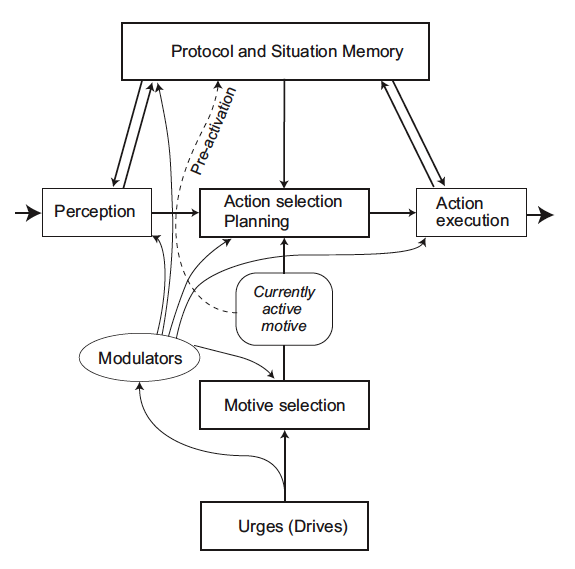
\includegraphics[width=11cm]{figures/Psi.png}
\caption{High-Level Architecture of the Psi Model}
\label{fig:Psi}
\end{figure}


\subsubsection{Emotion and Personality in the Psi Model}{}

\subsubsection{Psi in OpenCog}{}

\subsubsection{Goals in OpenCog}{}

\subsubsection{Execution Management}{Execution Management}

\subsection{The CogDial Dialogue System Architecture}{}

下面我们来介绍基于上述的目标控制体系的智能会话系统CogDial的系统框架。目前该系统只能处理英文对话,接下来章节中的对话的例子基本按照英文的习惯举的例子,可能不太适合中文的习惯,但是该系统的所采用的技术和理论基础都是完全适合中文的。CogDial主要采用了以下技术:

\begin{itemize}
\item  基于OpenPsi以及相关OpenCog机制的宏观规划(Macroplanning)
\item  本文第4章描述的句法分析和语义关系及逻辑关系抽取的自然语言理解技术
\item  本文第5章描述的微观规划(Microplanning)和表层生成的自然语言生成技术
\item  专门设计的符合智能会话系统的“言语行为规划器”集合,这些言语行为规划器将用于:
\begin{itemize}
    \item 在OpenPsi的控制机制下,结合当前的语境,激活相应的言语行为规划器
    \item 收集相关内容,生成能关联Microplanner的Atoms
    \item  调用一系列的认知机制(包括用于逻辑推理的PLN),选择相关的Atoms发送到Microplanner
\end{itemize}
\end{itemize}

\subsubsection{针对对话控制的OpenPsi的配置}{Configuring OpenPsi for Dialogue Control}

基于Psi的基本框架,我们选择了以下的具体需求用来指导我们的对话系统的行为:
\begin{itemize}
\item 社交需求(Affiliation):与他人互动,希望被其他成员接纳的需求;取悦谈话对象可以视为此目标的一个特例
\item 能力需求(Competence):通过对话达到某种目标的需求,衡量言语表达方式的指标
\item 确定性需求(Certainty):智能体对自身语境的了解需求,特别是对目标的了解需求
\item 新颖性需求(Novelty):维持智能的会话而不是简单重复的问答会话。
\end{itemize}

CogDial中的对话控制主要通过不同的需求来选择相应的言语行为规划器,因此,在选择言语行为规划器前,我们需要知道当前状态下上述每种需求的被满足的程度。鉴于目前的CogDial系统的有限能力,为了能更好地实现一个面向集成认知体系的智能会话系统框架,我们将上述的几项需求做了更具体化的定义:

\begin{itemize}
\item 社交需求(Affiliation):我们对该需求进行了下面三种满足程度:
\begin{itemize}
\item 当对话系统正在与人或者其他智能体进行会话时,该需求在一定程度上被满足;
\item 当系统正与多个人或智能体进行会话时,该需求被满足的程度提升;
\item  当该系统的会话内容都属于积极向上的时候(通过情感分析技术实现),该需求被满足的程度达到最高。
\end{itemize}
\item 能力需求(Competence):此项需求需要通过OpenCog来评估。简单来说,对每一个目标,OpenCog记录着会话系统在过去完成该项目标的程度,然后根据当前的不同目标所占的权重,我们可以通过以下公式估算该需求被满足的程度(XXX公式描述XXX 首先针对每一个目标,计算目标权重*能达到该目标的概率,然后求总)。当然计算目标被完成的程度,还应该考虑实现目标的语境等因素,目前我们的系统更注重构建一个智能会话系统框架,因此在语境无关的假设下来衡量目标被实现的程度。
\item 确定性需求(Certainty):如果会话系统正在和一个陌生人对话,或者系统无法理解大量被提及的单词或概念,那么当前的确定性需求被满足的程度就会降低。如果系统获取了新的可靠知识,那么该需求被满足的程度就会增加。
\item 新颖性需求(Novelty):我们定义了以下几种方式来增加智能绘画系统对新鲜度需求的满足程度值:
\begin{itemize}
\item 多和不同的人类或智能体会话;
\item 谈论新的话题或引入新的词汇和概念;
\item 学习新的可靠信息( OpenCog推理得出的新的置信度高的知识存储的载体原子(Atoms))
\end{itemize}
\end{itemize}

基于上述目标需求的智能会话系统,除了需要结合前文所述的OpenPsi的框架理论,以及本文描述的自然语言理解和生成的相关工具之外,还需要有以下模块:
\begin{itemize}
\item 制定一组能被特定目标需求激活的对话控制程序
\item 建立目标和相应去实现目标的行为之间的关联,可通过相关规则来实现,也可以通过强化学习来实现,我们系统框架采用两种结合的方法,但目前的系统还是以规则关联为主。
\end{itemize}


%%%%%%%%%%%%%%%%%%%%%%%%%%%%%%%%%%%%%%%%%%%%%%%%%%%%%%%%%%%%%%%
\subsubsection {言语行为规划器}{Speech Act Schema}
\label{sec:SAS}
%%%%%%%%%%%%%%%%%%%%%%%%%%%%%%%%%%%%%%%%%%%%%%%%%%%%%%%%%%%%%%%

“言语行为规划器”(Speech Act Schema)是CogDial的一个核心设计, 每个言语行为规划器里包含一种特定的言语行为(Speech Act),以及与该言语行为对应的特定的认知行为(Cognitive Procedure)。每种言语行为规划器都能在不同情况下被激发调用。对于言语行为规划器的选择,我们采用OpenCog中的OpenPsi的动机驱动模块来执行。

CogDial的总体规划是针对本文第2章综述里提到的42种SWBD-DAMSL言语行为[XXX],实现相应的言语行为规划器。 CogDial目前只实现了42种中的部分言语行为对应的言语行为规划器。另一方面,CogDial中的言语行为规划器的设计也绝不局限于这42种言语行为,CogDial实现了一些言语行为规划器能对应这42种中的某两种或多种言语行为,比如我们利用真值回答规划器(TRUTH VALUE ANSWER schema)来同时关联其中的YES QUESTION和NO QUESTION,从而可以将一般疑问句的回答根据真值的大小延伸到“可能”“不确定”“可能不”等,而不仅仅是局限于回答“是”或者“不是”。CogDial还根据智能体的具体情况拆分了这42种中的某些言语行为,例如,我们针对言语行为“STATEMENT” 实现了两个不同的言语行为规划器:回应声明以及智能体自发的用于表达其自身状态和想法等的声明。

总的来说,本文虽然没有完全照搬SWBD-DAMSL的言语行为分类,但是,该分类体系是来源于对大量人类会话的进行具体分析后的实验结果,也在具体的会话分析和抽象的言语行为理论之间架起了桥梁,使得抽象的言语行为理论在机器上实现变得可行,因此,SWBD-DAMSL的言语行为分类体系还是很有借鉴价值的。

要实现上述的言语行为规划器,每一个言语行为都会引发一个相应的认知行为,也就是说,每一个言语行为都会触发调用一段程序;而这样的机制正好符合OpenCog里的 GroundedSchemaNode的用法。GroundedSchemaNode是OpenCog的超图知识库里的一种节点类型,通常被封装在ExecutionOutputLink里,连接着一段代码(一般情况下是Scheme或者Python编写的代码)的名称。该代码可以通过ExecutionOutputLink被触发和执行。因此,鉴于这样的执行机制,我们可以通过对每个言语行为规划器定义一个GroundedSchemaNode来实现言语行为规划器。这样的设计方案可以减少冗长复杂的代码块,而直接通过OpenCog中统一又通用的Atomspace的基本操作方法来管理和执行复杂的言语行为规划器。另外,这样的机制也能很容易调用知识库Atomspace之外的复杂程序,从而得到很好的扩展性,也为言语行为规划器的扩展研究搭建了个很好的平台。例如,我们可以通过调用外部程序将逻辑推理系统PLN的前向或者后向推理应用到言语行为规划器中,使其能实现自适应学习,不断完善言语行为规划器。本文后面会进一步讨论这样的扩展。

每一个言语行为规划器的输入是一个被叫做对话节点(DialogueNode),DialogueNode是可以表示一方或者多方之间的会话交互的节点类型。DialogueNode可以有不同话语节点(UtteranceNodes)作为成员,在实现方式上,DialgoueNode通过MemberLinks指向不同的UtteranceNodes。而UtteranceNode则可以关联以下不同类型的节点:
\begin{itemize}
\item 关联一个或多个文本节点(TextNode)、句子节点(SentenceNode)或者短语节点(PhraseNode),则表示输入的话语内容来自一个或者多个文本、句子或者短语。
\item  关联一个声音节点(SoundNode),则表示该话语来自外界声音。
\item  关联指向说话者的Link。
\item  关联指向对话语的补充信息的Links,这些补充信息可以是该话语的言语行为类型、与该话语相联系的情感等。
\item  关联指向产生话语的言语行为规划器,用于响应是什么触发该话语。
\item  关联一个或多个解析节点(InterpretationNode),这些解析节点可以是用来解析话语的语义和语用信息。
\end{itemize}

言语行为规划器的输出是连接了一系列相关联Atoms的SetLink,该输出会送入本文\ref{chap:generation}中描述的微观规划和表层生成等工具,从而产生相应的自然语言来回应输入的内容。言语行为规划器还会将输出的话语关联到产生该话语的DialogueNode,这样不仅仅是记录了会话的内容,还能用于智能体的强化学习和提高智能体的各种需求的满足度。
下面通过一个例子来解释上述的实现过程。假设有下面的简单对话:
\begin{verbatim}
Ruiting: How are you doing?
CogDial: I am fine
\end{verbatim}
这个简单的对话可用以下的Atoms来表示:

\begin{verbatim}

MemberLink
	UtteranceNode [555]
	DialogueNode [123]
	
MemberLink
	UtteranceNode [666]
	DialogueNode [123]
	
EvaluationLink
	PredicateNode "say"
	ConceptNode "Ruiting"
	UtteranceNode [555]

EvaluationLink
	PredicateNode "say"
	ConceptNode "me"
	UtteranceNode [666]
		
EvaluationLink
	PredicateNode "Textual Content"
	UtteranceNode [555]
	SentenceNode "How are you doing?"
	
EvaluationLink
	PredicateNode "Textual Content"
	UtteranceNode [555]
	SentenceNode "I am fine."
	
EvaluationLink
	PredicateNode "Utterance Type"
	UtteranceNode [555]
	ConceptNode "Interrogative"
	
EvaluationLink
	PredicateNode "Utterance Type"
	UtteranceNode [666]
	ConceptNode "Declarative"
	
AtTimeLink
	UtteranceNode [555]
	TimeNode "22:15:33 12/06/2014"
	
AtTimeLink
	UtteranceNode [666]
	TimeNode "22:15:47 12/06/2014"
	
EvaluationLink
	PredicateNode "Interpretation"
	UtteranceNode [555]
	InterpretationNode [22]
	
EvaluationLink
	PredicateNode "Interpretation"
	UtteranceNode [666]
	InterpretationNode [33]
	
	
MemberLink
	EvaluationLink
		PredicateNode "doing"
		ListLink
			ConceptNode "you"
			VariableNode "var1"
	InterpretationNode [22]
	
	
MemberLink
	InheritanceLink
		ConceptNode "I"
		ConceptNode "fine"
	InterpretationNode [33]
	
ExecutionLink
	GroundedSchemaNode "polite_banter.scm"
	ListLink
		UttteranceNode [555]
		DialogueNode [123]
	UtteranceNode [666]

\end{verbatim}

其中的命题也可以有多种选择,例如:

\begin{verbatim}
EvaluationLink
	PredicateNode "Conversation Partner"
	DialogueNode $D
	$X
\end{verbatim}

该命题为真,当且仅当,$X是$D其中一个话语的发言人。


\subsection{Initial Speech Act Schema and their Linkage to Goals and Contexts}{}

在 \cite{Twitchell2004}, 中,Twitchell和Nunamaker根据Searl的言语行为理论的经典分类,在对大量的人类会话进行经验分析后,将言语行为细分为42种。虽然此分类体系很有理论研究价值,但在实验过程中,考虑到实用智能会话系统的语境等因素,我们对这42种言语行为做了稍微调整,同时也在CogDial中添加了一些SWBD-DAMSL研究中没有出现言语行为。

即使在有明确的言语行为类型的情况下,仍然有很多种方法去构建一个智能会话系统。CogDial根据多个广泛的可扩展目标制定一些特定的设计决策,在这些决策基础上,系统能通过自适应学习方法自动改进,为能跳出传统的对话系统的研究方法搭建一个基础平台。为了搭建这样的系统,需要考虑的第一点是,对于每一个言语行为,都有相应的固定形式的认知内容被触发,也有相应的习惯性表达方式来表达该认知内容。

如果在类似的言语行为类型分类基础上构建一个简单的“聊天机器人”,一般通过更简单,不用加入很多认知处理,针对每个言语行为类型,输出直接的具体的话语,也同样能达到类似的效果。例如,对于言语行为类型Agree,可以编写简单的程序使智能体输出“同意(Agree)”或者“是的,我同意(Yes, I agree)”。目前,“聊天机器人”的概念很模糊。我们这里提到的“聊天机器人”范围也很广,可以是完全基于模板匹配的聊天机器人ELIZA[XXX],也可以是具有一些推理能力但是基本忽略语义理解的Siri[XXX]。但关键的一点是,我们设计的CogDial系统,是本着该系统能“理解”自己在说什么的理念,也就是说,该系统所产生的话语来自于内部的语义关系图,且该语义关系图和系统知识库中的其他语义关系图之间有着丰富的语义关系。我们希望系统能在一定程度上更深地“理解”自己在说什么,而不是只生成它不理解的字符串。在某些情况下,在不理解的情况下破口而出一些话语,尤其是习惯用语,也是可以接受的(其实人类有时候也会无意识地这么做),但这并不是大部分情况。

在CogDial系统的设计中,每一个言语行为都需要下列几项内容与之相应:
\begin{itemize}
\item 相应的目标和语境二元组(goal,context),表明何时该言语行为会被触发。
\item 相应的能生成相关信息的程序,产生由该言语行为引起的要传递给谈话对象的信息。
\item 一个或多个相应的“语义模板”,表明由该言语行为引发的相关认知内容。
\item 连接上述语义模板所在的Atoms和特定的句子实现的Atoms的Links,用于传送到Microplanning,从而生成相应的话语。
\end{itemize}

这样一来,通过编写一些抽象的语义形式和特定的会话习惯之间的匹配模式,便能构建出一个具有一定合理功能的智能会话系统,当系统学习了用不同的更复杂的表达方式去实现抽象的语义形式后,也就能在更大程度上“理解”会话内容。此外,这些抽象的语义形式除了与言语行为和目标需求相关联,还和其他不同的认知内容相关联,因此,系统会随着经验的增长而趋向成熟。
假设任何言语行为被触发都能增加下面表达式中的EvaluationLink的真值:
\begin{verbatim}
EvaluationLink
	PredicateNode "Currently Having Conversation"
	TimeNode T
\end{verbatim}
    其中,“T”表示当前时间。又假设上面表达式中的EvaluationLink和系统中多个顶层目标有关联(该假设对于某些应用也不总为真,那么在这样的情况下,这些不为真的关联的链的权重会根据具体情况被调为适当的值),也就是说,该系统能看到会话行为带来的价值。 因为每个言语行为都蕴含着这个EvaluationLink,所以每个言语行为都会影响系统的目标实现。一些言语行为会通过持续进行对话从而超标完成某个系统目标。这样的言语行为会在后面章节详述。
    下面会给出一些具体的例子进一步解析前面几段提到的Atoms。
\begin{verbatim}
ImplicationLink <.5>
	EvaluationLink
		PredicateNode "Currently Having Conversation"
		TimeNode $T
	EvaluationLink
		PredicateNode "Increase Knowledge"
		TimeNode $T
\end{verbatim}
上述超图片段表明,维持对话能在一定程度上满足系统目标“增长知识”,ImplicationLink的初始权重设为0.5,表明“当前有会话”蕴含系统目标“增长知识”只有0.5的概率。这个权重会随着系统的经验而改变,也会通过其关联的其他节点和链的具体情况推算得来。例如:
\begin{verbatim}
ImplicationLink <.1>
	ANDLink
		EvaluationLink
			PredicateNode "Currently Having Conversation"
			TimeNode $T
		EvaluationLink
			EvaluationLink "DialoguePointer"
			PredicateNode "Currently Having Conversation"
			DialogueNode $D
		EvaluationLink
			PredicateNode "Conversation Partner"
			ConceptNode "Bob"		
	EvaluationLink
		PredicateNode "Increase Knowledge"
		TimeNode $T
\end{verbatim}

上面的超图片段表明,当进行对话的对象是Bob的时候,只有0.1的概率能实现系统目标“增长知识”。
\begin{verbatim}
ImplicationLink <1>
	ExistsLink $G, $S, $O, $U, $D
		ANDLink
			MemberLink
				GroundedSchemaNode $G
				ConceptNode "Speech Act Schema"
			AtTimeLink
				TimeNode $T
				ExecutionLink
					GroundedSchemaNode $G
					$S
					$O
			MemberLink
				UtteranceNode $U
				DialogueNode $D
			EvaluationLink
				PredicateNode "Textual Content"
				UtteranceNode $U
				SentenceNode $O
			AtTimeLink
				TimeNode $T
				EvaluationLink
					PredicateNode "Currently active"
					DialogueNode $D			
		EvaluationLink
			PredicateNode "Currently Having Conversation"
			TimeNode $T
\end{verbatim}

上面的例子说明,如果一个言语行为规划器被执行,当前的对话节点(DialogueNode)$D$会关联一个谓词“当前活跃”,表明$D$出于活跃状态, 那么“当前有会话”的目标被实现。

\begin{verbatim}
MemberLink
	GroundedSchemaNode "answer_yes.scm"
	ConceptNode "Speech Act Schema"
\end{verbatim}

接下来的例子演示了言语行为如何与目标关联:

\begin{verbatim}
ImplicationLink <.8>
	ExistsLink $S, $O, $U, $D
		ANDLink
			AtTimeLink
				TimeNode $T
				ExecutionLink
					GroundedSchemaNode "answer_yes.scm"
					$S
					$O
			MemberLink
				UtteranceNode $U
				DialogueNode $D
			EvaluationLink
				PredicateNode "Textual Content"
				UtteranceNode $U
				SentenceNode $O
			AtTimeLink
				TimeNode $T
				EvaluationLink
					PredicateNode "Currently active"
					DialogueNode $D			
		EvaluationLink
			PredicateNode "Please Conversation Partner"
			TimeNode $T
\end{verbatim}

上面的例子表明言语行为规划器“肯定回答”(”Answer Yes”schemma)可以用于增加实现“取悦谈话对象”目标的幅度值,超越了谈话对象因单纯继续对话而被取悦的程度。

许多言语行为规划器都会有不同的清晰表达相关语义内容的方式。比如说,一般会话的开头,可以说“你最近状态怎么样?”(”What has your state been recently?”),或者“你最近都忙什么?”(“What have you been doing?”) 等,而类似这样的语义内容很容易约定俗成地被说成“最近怎么样?”(“What’s up?”)。对于机器来讲,如果对话系统直接问 “What’s up?” 当然也没问题,但是有必要使系统知道 “What’s up?”只是其他两种说法或者 “what are you thinking about?“的一种约定俗成的简约说法。系统会根据智能体的不同个性对每种不同的说法一个相应的权值。

一般来说,会存在很多的“个性参数”影响着多种言语行为。在CogDial的实现过程,我们针对那些对对话影响较大的关键特性(我们称为“对话特征”(Dialogue-trait))创建相应的概念节点(ConceptNode),比如:习惯用语(Idiomaticity)、非正式(Informality)、精确(Precision)、累赘(Wordiness)、开放(Openness)。用来表示由言语行为规划器产生的具体话语的SetLink,将以不同的权重与这些表示不同对话特征的ConceptNode相连。例如,表示“I dunno”的SetLink将以较高的权重与“Informality”以及“Idiomaticity”关联,以较低的权重与“Precision”“Wordiness”关联。这些对话特征的参数可以在对CogDial设置基本参数的时候根据不同的需求人为设计。也可以在对话过程中根据谈话对象的喜好来自适应地调整。

综上所述CogDial的整个设计方案中,需要人工参与的部分包括:
\begin{itemize}
\item 自然语言理解流水线中的提到的规则(最终会被我们正在研究的无监督语言学习所取代,本文第9章有更详细的阐述)
\item OpenPsi中的顶层目标
\item 不同的言语行为所引发的不同认知过程。目前这些过程是在与GroundedSchemaNode绑定的相应Scheme或者Python代码中被实现。这些认知过程也可以在OpenCog的知识库Atomspace里被实现(如下文中的Question-answering schema)。
\end{itemize}
本章接下来的部分将进一步阐述CogDial使用的一系列言语行为规划器以及解释它们在CogDial中的实现机制,这些言语行为规划器大部分从SWBD-DAMSL中借鉴。当然这些特殊的言语行为规划器的集合并非一成不变,在以后对系统的不断改进和完善过程中,无疑会导致对该集合一定程度的延伸和细化。但我们相信这是一个好的开始,需要重申的是这些言语行为规划器分类是大量人类对话的实证分析的结果。目前,我们的研究工作重点在问答式规划器(Question-answering schema),将会在\ref{sec:QA} 中进一步阐述。



%% 参考文献
\bibliographystyle{reference/xmuthesis2}
\bibliography{reference/reference}

%% 发表的论文
\begin{publications}{2} % 这里的2是发表刊物的数量,用于计算需要缩进的长度用
    \item 第一作者, 第二作者, 第三作者.
        文章名一.
        刊物, 2009, 08:10-13.
    \item 第一作者, 第二作者, 第三作者.
        文章名二.
        刊物, 2009, 09:20-23.

\end{publications}


%% 最后致谢一下
\begin{thanks}
    谢谢父母

    谢谢导师

    谢谢朋友

    谢谢同学

    谢谢其他人
\end{thanks}


\end{document}
